\documentclass{article}
\usepackage[utf8]{inputenc}
\usepackage[T1]{fontenc}
\usepackage{url,hyperref,lineno,microtype,subcaption, todonotes}
\usepackage{longtable}
\usepackage{array}
%\linenumbers
% Bibliography handling
\usepackage[style=apa, backend=biber]{biblatex}
\renewcommand{\cite}[1]{\parencite{#1}}
\addbibresource{references.bib}
\renewcommand\refname{References} % Renames "Bibliography" (default) into "References"

%\usepackage[nottoc,numbib]{tocbibind} % Adds bibliography entry to toc
%\renewcommand\refname{Bibliography} % Renames "References" (default) into "Bibliography"
%
\hypersetup{
 colorlinks=true,
 citecolor=teal,
 linkcolor=blue
}
\usepackage{makeidx}
\makeindex

\newcommand{\question}[2]{{\color{red}[@#1: #2]}}
\newcommand{\contributed}[1]{%
    \par\noindent
    \begingroup
    \setlength{\leftskip}{1em}%
    \itshape
    Contributors: #1
    \par
    \endgroup
    \vspace{0.5em}
}

\title{Aurora Handbook for Citizen Science}
\author{ARCTICS Working Group}
\date{October 2024}
\begin{document}

\maketitle
\tableofcontents
\newpage

\section{Preface}
%\contributed{Maxime}
\textit{This project was supported by the International Space Science Institute (ISSI) in Bern, Switzerland through the ISSI Working Group ARCTICS - \href{https://collab.issibern.ch/arctics/}{Auroral Research Coordination: Towards Internationalised Citizen Science.}}\footnote{https://collab.issibern.ch/arctics/}\index{ARCTICS}\\
\textit{Core contributors to the handbook: Katie Herlingshaw, Donna Lach, Rowan Dayton-Oxland, Emma Bruus, Eero Karvinen, Vincent Ledvina, Noora Partamies, Maxime Grandin, Toshi Nishimura, Dave Knudsen, Marjan Spijkers, Les Ladbrook, Carlos Martinis, Bea Gallardo-Lacourt, Alan Dyer, Lena Mielke, Chris Ratzlaff, Lisa Evans, Matti Helin, Jeremy Kuzub, Mathieu Barthelemy, Neethal Thomas, Eric Donovan, Minna Glad, Mikko Syrjäsuo, Sophie Cordon.}\\
\textit{This work is licensed under a Creative Commons Attribution-NonCommercial 4.0 International License (CC BY-NC 4.0).}

 
\section{Welcome}
%\contributed{Rowan}
Welcome to the {\bf Aurora Handbook for Citizen Science}, a guide intended to bridge the gap between professional and citizen scientists who observe the aurora. Our objective is to empower the citizen community with the knowledge and tools to contribute meaningfully to auroral science, and to enable professional scientists to fully utilise the data and expertise of citizen scientists. By bringing together these two groups we aim to foster a strong collaborative relationship, and to use our shared data and expertise to advance our understanding of the aurora, a phenomenon which captivates and inspires us all. 

% Text box not converted to rst --> html
\subsection{Citizen Scientists}\index{citizen scientist}

\textit{A} \textbf{citizen scientist} \textit{is someone not engaged professionally to work on a project as a scientist, who contributes to scientific research as a volunteer or other collaborator (paid or unpaid). They can be school students, teachers, families, retirees (including retired scientists), researchers contributing outside their own field, independent researchers, or other members of the general public.}\\
\\
Citizen scientists can collaborate with professional scientists at different levels -- they may collect and/or analyse data for the project (contributory citizen science), or they may collaborate with professional scientists on many different parts of the project (collaborative citizen science). They may also design the project with professional scientists from the ground-up (co-created citizen science). Other types of citizen science projects may be initiated by a community, with scientists acting as external consultants (contractual citizen science), and additionally independent researchers may collect their own data, or conduct their own research, and ask professional scientists for advice or assistance (collegial citizen science). Historically, auroral citizen science projects have included members of the wider community in many of these ways. This Handbook will help you anticipate what to expect in your collaborations with professional scientists.

% Text box not converted to rst --> html
\subsection{Scientists}\index{ scientist}

\textit{A} \textbf{scientist} \textit{is a trained expert who is paid and employed at an institution to study the natural world. It is their profession to employ the scientific method to analyse the natural world and publish their results through reputable, peer-reviewed journals.}\\
\\
As a professional scientist, you have many opportunities to leverage observations made by citizen scientists of phenomena associated with aurora. This Handbook will help you anticipate what to expect in your conversations with citizen scientists and how to seek the data you are looking for. For example, suggesting ``your photos will get exposure'' will often result in a negative response. Instead suggesting their work will ``contribute to emerging science'' and that they will be ``included as a co-author'' will receive a more favourable response.

\subsection{Both}
Combining the communities of citizen scientists and professional scientists in studying aurora creates a unique opportunity to leverage the strengths of each group. Citizen scientists, with their diverse geographical locations and dedication to observation, provide a resource that would be difficult for professionals to gather alone. Professional scientists, in turn, offer the expertise needed to interpret these observations and draw conclusions. Together, they form a partnership where the data collected by citizens support scientific research, leading to new discoveries, more thorough studies, quicker advancements, and a better understanding of auroral phenomena.

% Section numbers not converted to rst --> html so this may need to change...
%\paragraph{Practical note for readers:} This document includes section references formatted as (see X.Y), where 'X.Y' represents the relevant section number. Each link will lead you to the respective section for more detailed information.

\subsection{Testimonials}

\textit{I have been involved in auroral citizen science since about 2015, and it has been so rewarding connecting with the scientists who study the aurora and learning from them. I was hesitant to speak up at first, but once I got comfortable, I realised how valuable it is for the scientist to be able to hear about my observations. I look through thousands of my aurora photos over and over again and have so many questions. The scientists use satellite data and other mechanisms to make their analysis without the benefit of thousands of photos from an event. I have been in conversations with the ARCTICS and Aurorasaurus teams when together we discovered the answer to some of these questions and potentially made new discoveries. As the ARCTICS team works on this handbook, I see how much we are learning from each other during every meeting. This is the reason I am here.
}\\
--- Donna Lach, Manitoba, Canada\\
\\
\textit{ARCTICS has been an incredibly enriching and positive experience. As a researcher specialising in a narrow field, I was amazed by the diverse auroral phenomena that citizen scientists can observe and identify, even within a single evening. Although I’ve had the opportunity to see auroras, my limited experience in photographing them has often prevented me from reviewing what I witnessed. ARCTICS has provided a window into the unique experiential perspective of a citizen scientist, in which I recognise the huge potential for advancing scientific research. I’ve been impressed by the dedication and knowledge of the citizen scientists and I learned a lot from them as we collaborated on the handbook.}\\
--- Katie Herlingshaw, Longyearbyen, Svalbard\\

\textit{A whole new aspect of aurora-hunting has opened to me, as a newbie in citizen science. Learning more about the aurora and contributing to space weather science enriches the experience of seeing and photographing the aurora. My contribution started mostly by listening and reading, but after a while I discovered that I have practical experience and lots of pictures to contribute. The contact with other aurora addicts like me, both scientists and citizen scientists from all over the world, is a huge bonus. It takes aurora hunting to a next level.}\\
--- Marjan Spijkers, Zwolle, Netherlands
\\

\textit{When we started the ARCTICS collaboration in September 2023, I was far from imagining how stimulating a journey it would be. When you bring in the same room (or videocall) people from very diverse backgrounds and experiences but all driven by the same curiosity to understand the aurora and associated physics, truly, the magic happens! How many times have we been puzzled looking at a photograph, realising how little we actually understand the upper atmosphere and its interactions with space... It is extremely humbling to be part of such a collaboration and constantly learn from everyone. What has been making ARCTICS so fruitful, I believe, is the overall positive and friendly atmosphere, in which every participant feels safe to speak, be it to make a suggestion or to ask a question. Curiosity, humility, respect; those three adjectives can definitely lead to both fantastic discoveries and lasting friendships!}\\
--- Maxime Grandin, Helsinki, Finland\\


\section{Introduction}

\subsection{What is the Aurora?}\label{what-is-aurora}\index{aurora!definition}
%\contributed{Dave, Vincent}
\begin{figure}
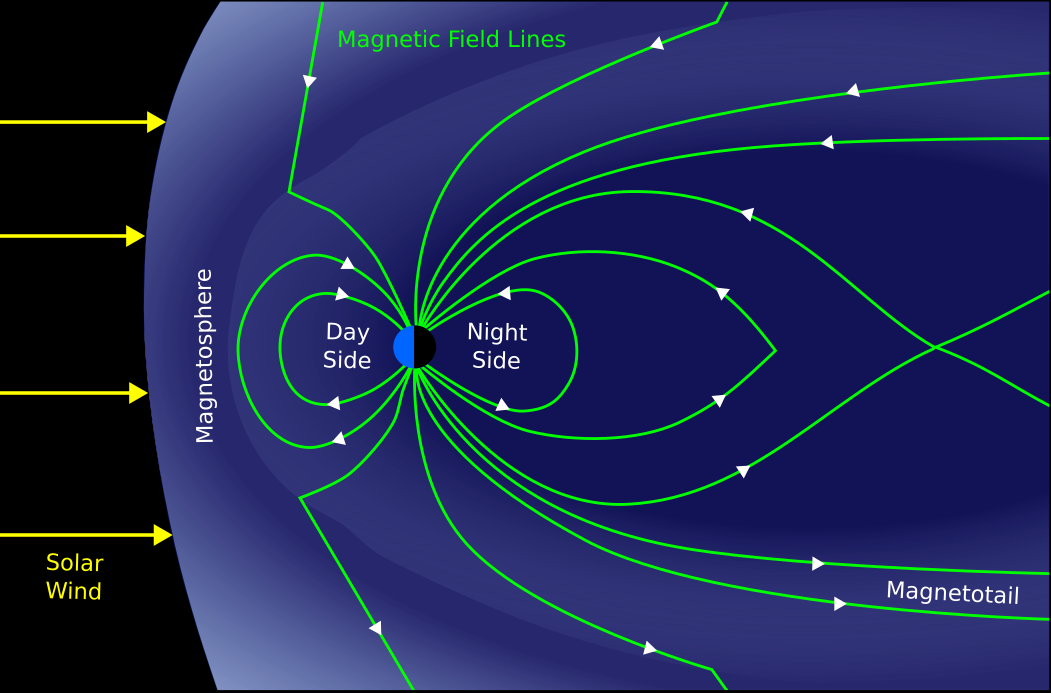
\includegraphics[width=\linewidth]{Fig1_magnetosphere.png}
\caption{The Earth's magnetosphere contains the Earth's magnetic field and is a source of protection from the solar wind. Image credit: Katie Herlingshaw.}
\label{fig-magnetosphere}
\end{figure} 

Surprisingly, this seemingly simple question is still a matter of debate among scientists, despite the fact that scientific descriptions go back as far as Galileo (1619), who wrote:\\
\textit{``...many of you will have seen, more than once, the sky in the night hours, in parts towards the north, illuminated in a way that the clear [sky] does not yield to the brighter aurora, far from the rising Sun.''}\\
Of course we now know that the aurora encircles both the northern and southern polar regions. The essential elements of the definition are thus lights in the nighttime sky, predominantly in polar regions. This raises the question: ``Why polar regions?'' The answer was not available in Galileo's time. It had to wait for major developments in the science of electricity and magnetism. 

Key among these discoveries were that the Earth is essentially a giant magnet, and that the space enveloping the solar system and Earth (interplanetary space) is not empty but filled with a stream of charged particles (the solar wind), like a gentle breeze buffeting the Earth. The magnetic fields of Earth also extend into outer space forming a sort of shield that deflects solar wind like a rock causes water to divert around it in a river. In the case of the rock, a tiny protective area of slow current is carved away from the surrounding faster water. In the case of the solar wind flowing around Earth, the magnetic pressure forms a protective shield that is otherwise known as the magnetosphere, shown in Figure~\ref{fig-magnetosphere}. The interaction between the solar wind and Earth's magnetic field lead to large systems of electric currents coursing through Earth's magnetosphere and the upper polar atmosphere. 

It was Kristian Birkeland in 1913 who first made the connection between the aurora and electric currents in the upper atmosphere, based on magnetic measurements from the ground. It was not until the dawn of the space age that \textcite{McIlwain1960} demonstrated with rocket measurements that these currents are carried in some cases by electrons accelerated along Earth's magnetic field lines into the atmosphere. Space physicists refer to this process as ``particle precipitation'', but instead of water, it is charged particles raining down from above. When they collide with atoms and molecules in the upper atmosphere (mostly oxygen and nitrogen), light is created that we perceive as the aurora. By examining the chemical ``fingerprints'' of these light emissions (a science called spectroscopy), it was discovered that some auroral emissions are due not only to electrons, but rather protons from Earth's magnetosphere streaming downwards along Earth's magnetic field \cite{Vegard1939}, creating a distinctive type of aurora (see \ref{proton-aurora}).  

More recently, the discovery of ``STEVE'' (see \ref{steve-sar-arcs}) \cite{MacDonald2018} revealed the possibility that charged particles leading to auroral emissions may be energised within the upper atmosphere itself, through electric fields that are channelled from the magnetosphere into the atmosphere via Earth's magnetic field.

It is often claimed that the aurora is \textbf{exclusively} caused by energetic charged particles from the Sun. In other words, the solar wind directly strikes the atmosphere, causing auroral emissions. Although this is true in two small dayside regions known as the ``cusps'',  it is inaccurate for most of the aurora we observe. Through processes that are largely outside the scope of this handbook, Earth's magnetosphere channels {\it energy} -- but not necessarily particles -- from the solar wind into the magnetosphere and upper atmosphere.   
Proof that auroral particles do not come directly from the solar wind can be seen in the fact that the particles that drive the aurora on the nightside of the planet tend to have hundreds or thousands of times more energy than particles arriving from the Sun, though there are exceptions \cite{Hosokawa2024}. In fact, a significant portion of magnetospheric (and therefore auroral) particles may originate not from the Sun at all, but from Earth's upper atmosphere and ionosphere \cite{Chappell1987}. Tracing the exact origins of the particles responsible for auroral emissions requires collaboration among many sub-disciplines, including ionospheric, magnetospheric, interplanetary, and solar physics. For the most part, the key elements of the aurora, including the characteristic shapes and energies of its drivers, originate in the immediate space surrounding the planet within Earth's magnetosphere. 
So, to modernise Galileo's definition: \\
% Text box not converted to rst --> html
\newline
%\noindent\fbox{%
%    \parbox{\textwidth}%
%} 
\newline

In this case ``energetic'' means having more energy than particles comprising the surrounding, undisturbed upper atmosphere. This definition distinguishes aurora from airglow, which is an emission of light from atoms and molecules in the upper atmosphere, but occurring at all latitudes, and which is driven by solar ultraviolet light and chemical processes. Airglow also tends to be much weaker than the aurora at visible wavelengths and is also almost never visible to the unaided eye. This definition of aurora also excludes lightning, which is driven by charged particles and electric fields, but at all latitudes and altitudes within the atmosphere. The idea of this definition aligns well with an earlier discussion by \textcite{clarke2004}.

In this definition, we try to encompass both traditional aurora and newer features that have been described previously as ``aurora-like''. This is a choice that we have made for the purpose of clarity in this handbook but be aware that in scientific papers and media articles, categorisations can differ.


\index{atmosphere!upper}\index{charged particles}\index{magnetosphere!processes}


% section numbering not converted to rst --> html
% May require change in the style for "see X.Y" we use
\subsection{Why Study the Aurora?}\index{aurora!research motivation}\index{plasma physics}\index{climate}\index{atmospheric science}

\begin{figure}[h!]
  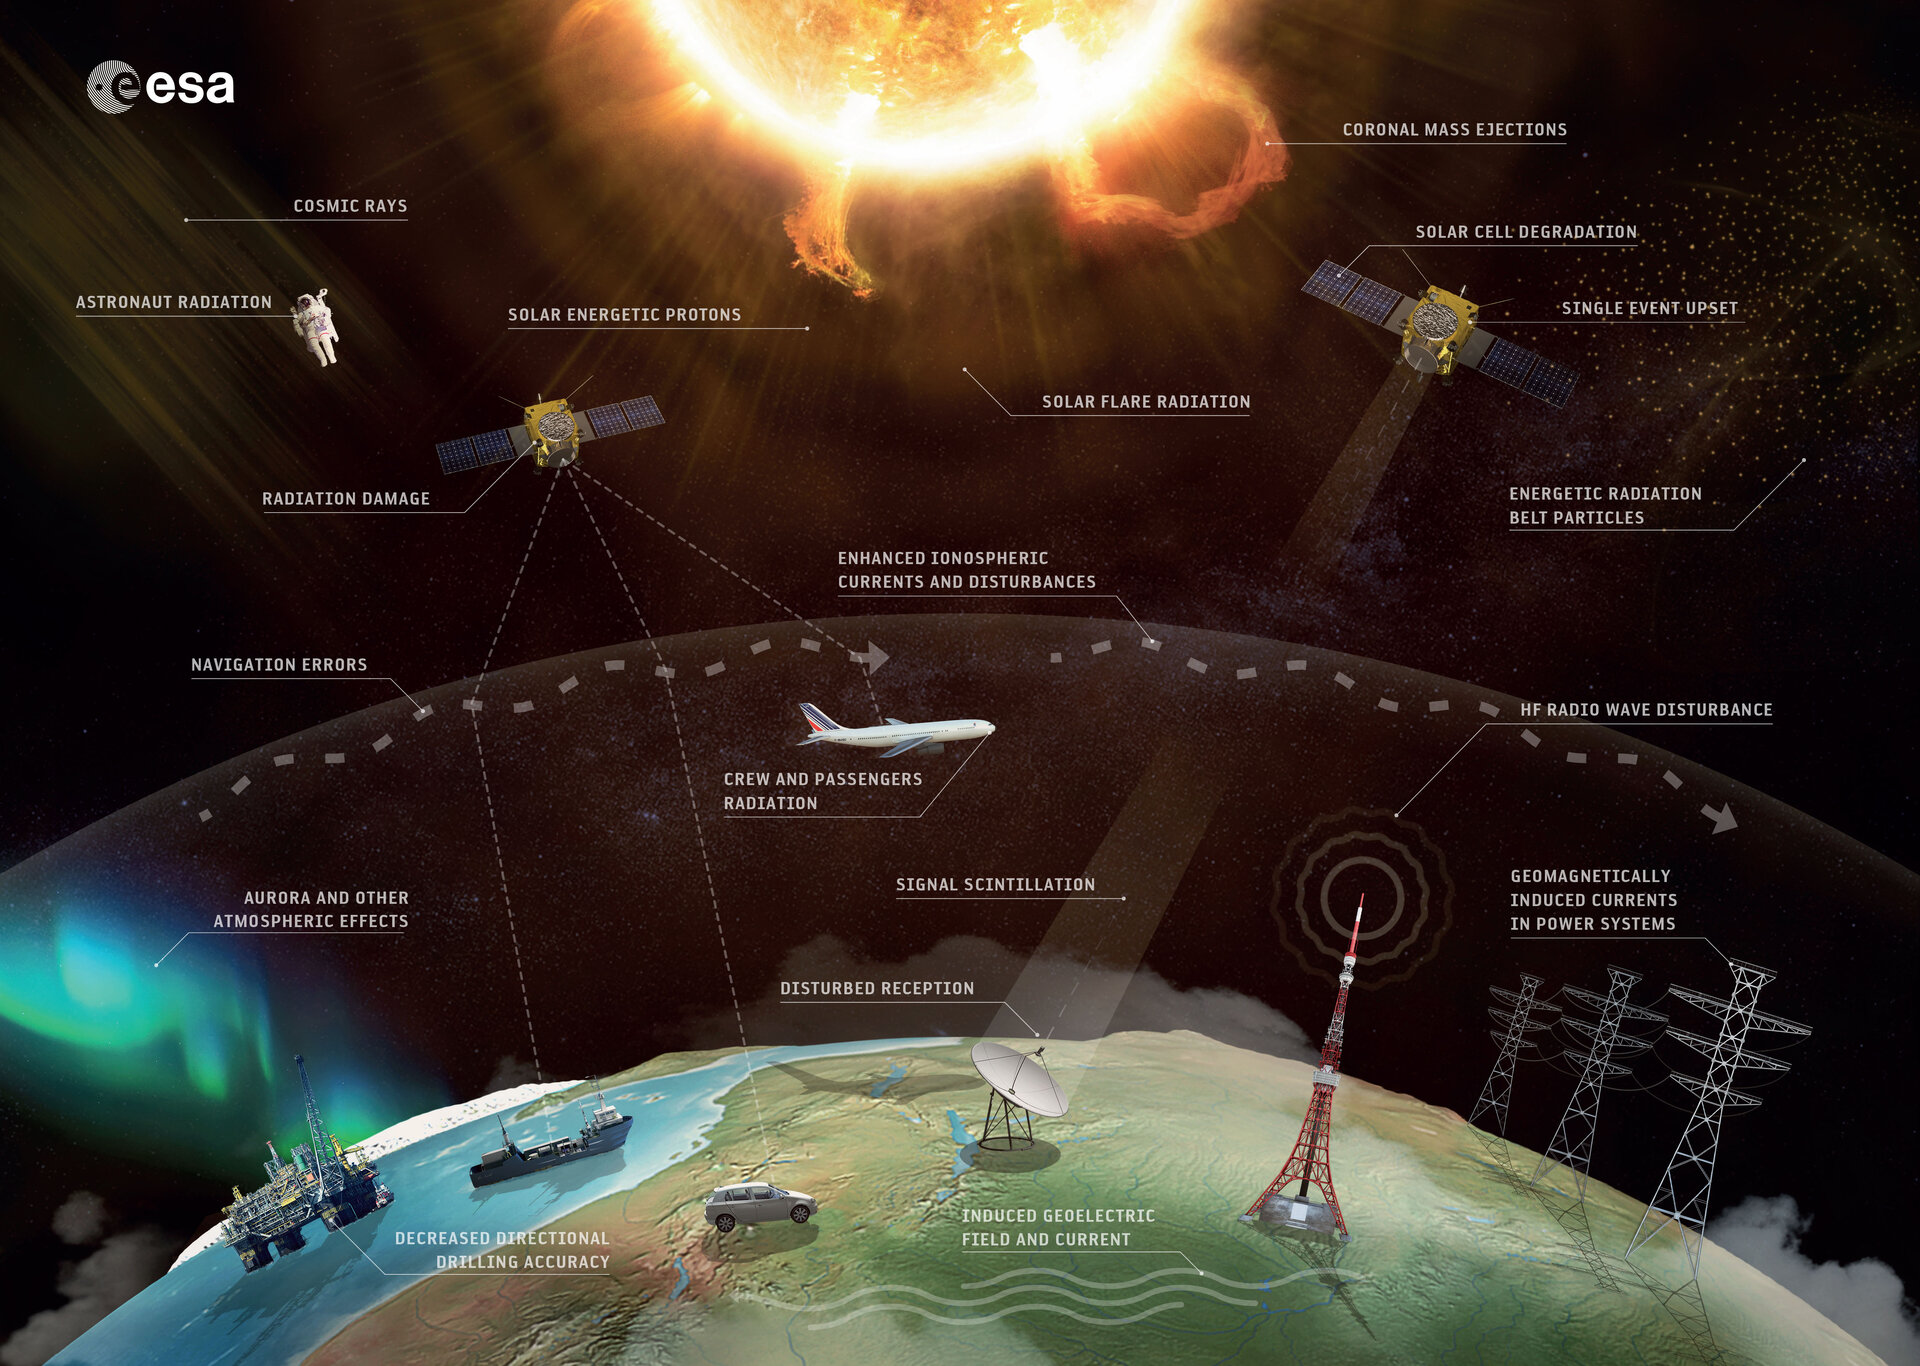
\includegraphics[width=\linewidth]{Fig2_SpaceWeather.jpg}
  \caption{Examples of space weather impacts on society. Image credit: ESA/Science Office, \href{https://www.esa.int/ESA_Multimedia/Terms_and_conditions_of_use_of_images_and_videos_available_on_the_esa_website}{ESA Standard Licence}.}
  \label{fig-space-weather}
  
\end{figure}

%\contributed{Rowan}
So why research the aurora? What insights can it offer us?\\
Firstly, \textbf{the aurora provides a natural laboratory for studying plasma physics}.
Plasma is an ionised gas made of free electrons and ions that respond strongly to electromagnetic fields. It makes up about 99\% of the visible matter in the universe and is not well understood compared to the other three states of matter (solid, liquid, gas). The magnetic environment of the Sun and Earth consists of a complex plasma environment where we can observe complicated plasma processes.
Plasma, which makes up about 99\% of the visible matter in the universe, is not well understood compared to the other three states of matter (solid, liquid, gas). The magnetic environment of the Sun and Earth consists of a complex plasma environment where we can observe complicated plasma processes. One very important method of understanding these plasma processes is by measuring the auroral emissions which result from them. Insights which help us to understand the range of different auroral forms and behaviours can be applied across the rest of plasma physics, from stars, supernovae and interstellar space in astrophysics, to lightning, fire, and fusion reactors, all the way to spacecraft ion-thrusters or the humble neon sign. Plasma is all around us, both in scientific research and day-to-day engineering, and aurora research provides a vital laboratory to help us fully understand it.

The aurora is also closely linked to \textbf{space weather}, such as solar storms. Understanding the aurora can improve our ability to predict space weather and the Earth's magnetic reaction to it. This is crucial for protecting satellites, communication systems, and power grids from solar-induced disturbances that can have significant impacts on modern technology and infrastructure. These effects are shown in Figure~\ref{fig-space-weather}.

Even closer to the ground, the aurora interacts with the \textbf{Earth's atmosphere}, influencing its chemical composition and temperature. By studying the aurora, researchers gain insights into atmospheric processes, including how energy is transferred from the Sun to the Earth's atmosphere and how it affects atmospheric chemistry. The aurora can also offer clues about the effects of \textbf{climate change} on the upper atmosphere. Changes in the Earth's upper atmosphere can be observed in the aurora and other atmospheric light emissions. By studying these interactions, scientists can better understand the broader impacts of climate change on the atmospheric system.




\subsection{Colours of the Aurora}


\begin{figure}[h!]
  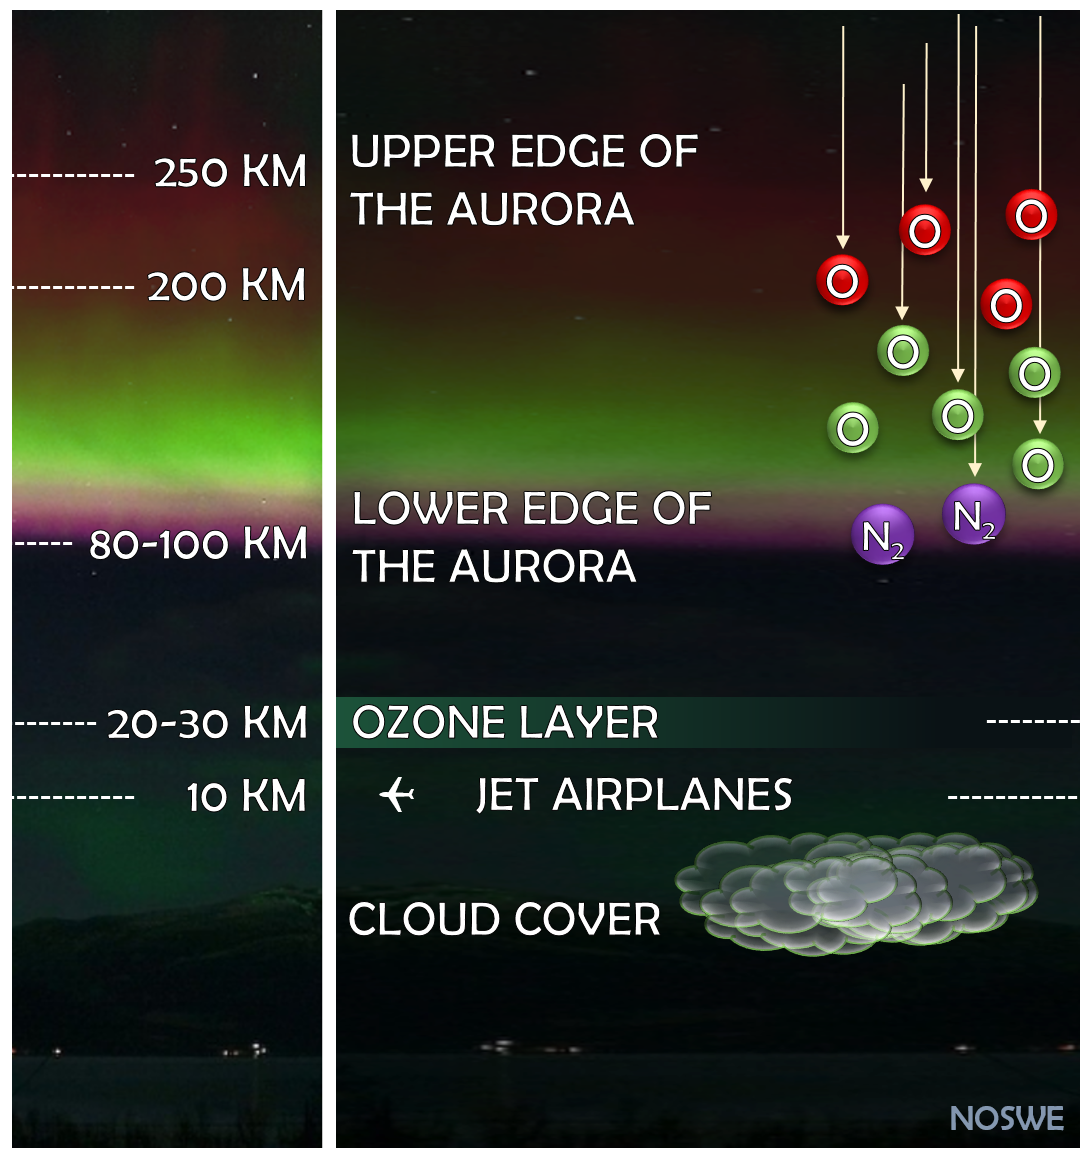
\includegraphics[width=\linewidth]{Fig3_Colours.png}
  \caption{Illustration showing the different auroral colours and altitudes. Image credit: Norwegian Centre for Space Weather (NOSWE). }
  \label{fig-colours}
  
\end{figure}

The colours of the aurora depend on the types of atmospheric gases that the incoming electrons collide with. At altitudes of about 100 to 200 km, the main gases are oxygen and nitrogen (both atomic and molecular forms). When electrons collide with these gases, they transfer energy, causing the gases to become excited. When they relax back to their normal state, they release light, which we see as the aurora. Figure \ref{fig-colours} shows the different colours emitted by oxygen and nitrogen at various altitudes in the ionosphere, where the aurora occurs. The altitudes where aurora happens is a section of Earth's atmosphere called the ionosphere.


Red auroral light comes from a low-energy transition in atomic oxygen (O). It is a slow emission, so it only occurs high in the atmosphere (above about 150 km) where the atmosphere is less dense. In this region, there is enough time for the gas to relax back into its normal state by emitting light, rather than the energy being transferred by collisions. Green light also comes from oxygen but from a higher energy level. This faster emission happens at lower altitudes, between 90 and 180~km.


Blue auroral light, which is called blue because of its position on the colour spectrum, is produced by ionised nitrogen molecules (N2+). It occurs at similar altitudes as the green light but is much fainter, often seen at the edges of fast-moving aurora, where green light fades into blue. 


A special conditions for blue light can occur when the upper part of the auroral curtain is lit by sunlight. In this case, the incoming electrons push nitrogen higher in the ionosphere, placing it at altitudes typical for red emissions. The illuminated nitrogen then re-emits the blue part of the sunlight spectrum through a process called resonance scattering, resulting in what is known as ``sunlit aurora''. This phenomenon can be observed shortly after sunset and just before sunrise when solar illumination is present.


\section{Aurora Chasing}
This section covers how to stay safe when taking aurora photos, how to decide when to go out, and advice on etiquette from seasoned aurora chasers.

\subsection{Staying Safe}\index{staying safe}
%\contributed{Donna, Marjan, Minna G}

As an aurora photographer, heading out into the dark requires thoughtful planning and preparation. To ensure a safe and successful experience, consider these tips.

\noindent\newline\textbf{Before You Leave:}
\begin{itemize}
    \item \textbf{Inform Someone:} If you are venturing out alone, let someone know your plans, including your location and expected return time. Share your GPS location via a phone app. Ideally, bring a friend to help keep an eye out for potential dangers and provide support if needed.
    \item \textbf{Preparation is Key:} Ensure your phone is fully charged and bring a charger. Do not forget to pack food and drinks to maintain your energy. Check that your vehicle’s fuel tank is full before departing, and pack a headlamp for visibility in low-light conditions.
    \item \textbf{Scout Your Location:} Visit your intended site during the day to identify potential obstacles, such as rocks or steep drop-offs. Be mindful of light pollution; tools like \url{www.lightpollutionmap.info} can help you find darker areas. Aim for a location that is safe for extended stays.
    \item \textbf{Access Permissions:} Confirm that you have permission to access your chosen location. Familiarise yourself with local laws regarding public and private property access, and select a site away from traffic.
    \item \textbf{Plan for Connectivity:} Cell service may be spotty in remote areas, so download maps before you leave. If you frequent areas with poor reception, consider a cell phone booster for your vehicle. For reliable communication and emergency assistance, consider purchasing a device that can send texts and trigger an SOS via satellite.
\end{itemize}

\noindent\newline\textbf{While You are Out There:}    
\begin{itemize}
    \item \textbf{Wear Reflective Clothing:} If photographing alone, opt for reflective clothing for safety. If shooting with a group, remember that reflections may appear in their photos.
    \item \textbf{Wildlife Awareness:} Be aware of local wildlife and take precautions to deter larger animals while protecting yourself from smaller pests. If you are away from your vehicle, consider having a spotter. Carry legal protection for larger wildlife, if necessary. Your hearing can be a critical defence—make noise or use a spotlight if you detect animals. If you are alone in a high-risk area, set up your camera and retreat to your vehicle, using an intervalometer or remote shutter release to monitor your shots.
    \item \textbf{Insect Protection:} To fend off mosquitoes and other pests, consider using a repellent device to create a bug-free zone while you work.
    \item \textbf{Footwear:} Slip-on boots are an excellent choice. They allow you to tuck in your pants for protection against insects and poisonous plants, and they make it easier to navigate through water or mud.
    \item \textbf{Cold Weather Precautions:} Stay warm during cold photography sessions by using heat packs inside your clothing. Mittens typically offer more warmth than gloves, but combining both allows you to easily remove mittens for camera adjustments. Dress in layers with wool, as trapped air provides great insulation. Pay special attention to your face, nose, ears, toes, and fingers, as these areas are especially vulnerable to frostbite. If you are out with other people, consider regularly monitoring each other's face for frostbite. If your boots have enough space, wearing two pairs of wool socks can enhance warmth significantly. A snug, windproof wool hat will also help retain body heat.
    
    When setting up your camera, position it outside the vehicle and use an intervalometer or remote shutter release from inside. Your running car can keep you warm, but be aware that it may muffle sounds, making it difficult to hear nearby wildlife. In extreme cold, prioritise safety over getting the perfect shot; always consider the windchill factor and dress appropriately. Being well-prepared allows you to enjoy your time outdoors longer. Additionally, keep a sleeping bag in your car as a precaution in case of a breakdown, ensuring you stay warm while waiting for assistance.
\end{itemize}

\subsection{Aurora Chaser Etiquette}
%\contributed{Marjan, Donna}
When chasing the aurora, it is important to be considerate of others around you. This means avoiding the use of bright lights, loud music, or any loud noises that could disturb the experience for others. Refrain from using high beams, and if possible, cover your camera's light sensor with black tape to prevent unnecessary light (such as the flash from the self-timer). Be mindful that using your camera’s live view function can disrupt others' night vision. If you go in and out of your vehicle during the observation, learn how you can shut off your car interior lights for this, or cover the front of your vehicle with a blanket. If possible, favour using red rather than white light with your headlamp, as red light is less disturbing for your (and others') night vision. As well as considering other people, be mindful of the environment and avoiding disturbing wildlife as much as possible, minimise the impact on the nature and vegetation around you, and take back all trash when you leave.

When reviewing your photos, if you are unsure about identifying a particular phenomenon do not make definitive claims. Instead, pose it as a question to encourage discussion. Be respectful when others seek your opinion on their photos, offering constructive feedback without being dismissive. Always ask for permission before sharing someone else's picture, ensuring you respect their ownership and effort.

\subsection{When to Go Out}\label{whentogoout}\index{aurora chasing!when to go out}
%\contributed{Vincent, Marjan}
The most common question is ``When should I go out?'' There is no simple answer for every person since the conditions required to see aurora depend on many factors such as cloud cover, geomagnetic activity, time of the year, and geographic location.

The sky must be dark and clear enough to see the aurora -- the aurora occurs high in the atmosphere above all major terrestrial weather. Seasonal cloud cover varies from place to place; look up the clearest months for cloud coverage in your target location. Although aurora can appear very bright against the inky backdrop of a night sky, they are dim compared to even a twilight sky. Therefore, it needs to be sufficiently dark to see the aurora. Look up the daylight times for your selected dates at your specific location online\footnote{\url{https://www.timeanddate.com/sun/}}. From these Sun graphs, you will see a description of different intensities of light: daylight, civil, nautical and astronomical twilight, and night. Optimally you should have long stretches of night at the time when you will be aurora chasing, but some amount of astronomical twilight is still acceptable levels for aurora photography. You should avoid all the other levels of light during your aurora chasing window.


\subsubsection{Moon Phase}
The phase of the Moon also affects the visibility of the aurora. Full or near-full phases may cause faint auroral forms to not be visible with the naked eye or on camera. However, bright auroral displays can be seen easily even with a full Moon in the sky. Ironically, it is easier to see colours and details of bright aurora under a full Moon. The added ambient light activates more colour- and detail-sensitive photoreceptors (cones) in your eye and allows for better colour perception. New or near-new Moon phases are best for seeing faint auroral forms as well as experiencing a higher contrast between the aurora and the background sky. For cameras, it is harder to see the dim auroral light in photographs when the Moon is up and full, as it is so much brighter than the aurora. The bright Moon dilutes the colours and overpowers the already poor contrast of the aurora to the background. In late winter and early spring at high latitudes, the first quarter Moon might not set, while the last-quarter Moon might never rise. In autumn the opposite is true — the first-quarter Moon is low or below the horizon while the last-quarter Moon rises early and climbs high into the sky. At lower latitudes, since the aurora is usually confined to the poleward horizon and fainter than seen directly under the auroral oval, new Moon will ensure you are able to see and photograph the entire show.

\subsubsection{Aurora Forecast}

\begin{figure}
  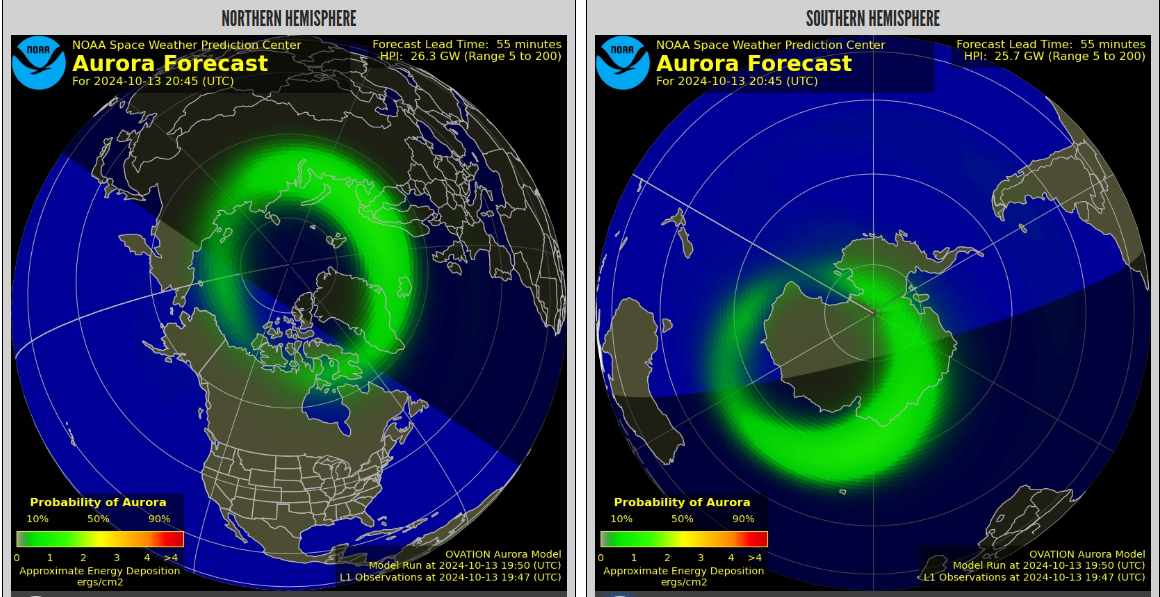
\includegraphics[width=\linewidth]{Fig5_auroralOvals_OvationPrime.png}
  \caption{Auroral ovals in the northern (left) and southern (right) hemispheres as forecast by the OVATION Prime model \cite{Machol2012} at 20:45~UTC on 13~October 2024.} 
  \label{fig-auroralovals}
\end{figure}

The auroral ovals are the rings of aurora that are centred around the magnetic poles in the northern and southern polar regions (see Fig.~\ref{fig-auroralovals} for an illustration). Being directly under the auroral oval provides the best viewing conditions for aurora displays. It is nearly impossible to predict the aurora more than one month out. Besides the correlation of the about 11-year solar cycle with the occurrence of aurora, the longest-range forecast is currently the \href{https://www.swpc.noaa.gov/products/27-day-outlook-107-cm-radio-flux-and-geomagnetic-indices}{NOAA SWPC 27-day aurora forecast}\footnote{https://www.swpc.noaa.gov/products/27-day-outlook-107-cm-radio-flux-and-geomagnetic-indices}. Forecasts often use the Kp Index as a measure of activity, where higher numbers represent an expanded and more active auroral oval (see \ref{kp-index}). The outlook predicts Kp values 27 days in advance. This is the same amount of time as one full solar rotation so the prediction is based on the last observed solar rotation. In short, this forecast tries to predict the occurrence of space weather phenomena called high-speed streams that occasionally persist for multiple solar rotations. The 27-day forecast is rarely accurate and should not be used beyond a general awareness of incoming solar activity.

The \href{https://www.swpc.noaa.gov/products/3-day-forecast}{NOAA 3-Day Aurora Forecast}\footnote{https://www.swpc.noaa.gov/products/3-day-forecast} is a far more useful tool for predicting active nights of aurora. This outlook takes high-speed streams into account as well as more transient space weather phenomena such as coronal mass ejections (more information on these space weather drivers can be found on the NOAA/SWPC webpages about \href{https://www.swpc.noaa.gov/phenomena/coronal-mass-ejections}{coronal mass ejections}\footnote{https://www.swpc.noaa.gov/phenomena/coronal-mass-ejections} and \href{https://www.swpc.noaa.gov/news/coronal-hole-high-speed-streams-ch-hss}{solar wind high-speed streams}\footnote{https://www.swpc.noaa.gov/news/coronal-hole-high-speed-streams-ch-hss}). Like the 27-day aurora forecast, there is uncertainty in the 3-day forecast. It is inherently hard to predict space weather on short timescales let alone days in advance, so do not take predicted Kp values literally but instead use the 3-day forecast as a guide to when generally enhanced activity might be expected.

The next major leap in forecasting ability comes at the minute-to-hour timescale. Here, solar wind parameters\footnote{https://www.swpc.noaa.gov/products/real-time-solar-wind} may be interpreted to forecast auroral activity. The \href{https://www.swpc.noaa.gov/products/aurora-30-minute-forecast}{NOAA SWPC OVATION Prime Model}\footnote{https://www.swpc.noaa.gov/products/aurora-30-minute-forecast} \cite{Newell2014} incorporates these solar wind parameters into an auroral oval model that updates every five minutes and aims to predict the strength of the aurora around 30 minutes in advance. The model outputs a shaded colourmap indicating percentage chances of viewable aurora overhead. A key point in using this model is understanding its limitations. OVATION Prime computes an average response of the aurora based on given solar wind parameters and thus smooths over rare, small, or transient auroral phenomena like STEVE and SAR Arcs (see \ref{steve-sar-arcs}), and fragments (see \ref{fragments}). OVATION Prime also does not model substorms. Even with these limitations, the model is easy to use and interpret for aurora chasing.

A smartphone prediction of the auroral occurrence based on the observer's (or given) location is provided by \href{http://kho.unis.no/Forecast.html}{Aurora Forecast 3D}\footnote{http://kho.unis.no/Forecast.html} \cite{Sigernes2011}. It places the auroral oval based on the observed or forecasted Kp values. A simple version \href{http://kho.unis.no/ForecastR.html}{Aurora Forecast Rocketeer}\footnote{http://kho.unis.no/ForecastR.html} uses the phone location information to show the local predicted sky view instead of prompting the user.

\subsubsection{Auroral Substorms}
\label{auroral-substorms}

\begin{figure}
  \includegraphics[width=\linewidth]{Fig4_substorm.jpg}
  \caption{Left: The development of the auroral substorm during the expansion and recovery phases is shown schematically \cite{Akasofu1964}. Right: The first series of global images of an auroral substorm observed by the Dynamics Explorer satellite \cite{frank1988}. The view in both cases is looking down onto the Earth's magnetic pole.} 
  \label{fig-substorm}
\end{figure}

Alluded to in the last section, the phenomenon called ``substorm'' is a major disruption of the nightside magnetic field of the Earth (the magnetotail, see Figure~\ref{fig-magnetosphere} generally producing spectacular auroral displays in the polar regions. Typically, substorms occur about 1000 times each year \cite{Partamies2013}, meaning that, on average, there is one every 8~hours. In practice, when geomagnetic conditions are active (for instance due to an incoming coronal mass ejection or high-speed stream), there can be several substorms during the same night. 

While every substorm is unique, they generally follow a certain pattern, known as the substorm cycle, shown in Figure~\ref{fig-substorm}. Described in the well-known work by Akasofu in 1964 \cite{Akasofu1964}, the auroral substorm is a three-part sequence consisting of a {\bf growth}, {\bf expansion}, and {\bf recovery phase}. The growth phase is characterised by thin, discrete auroral arcs that usually stretch from east to west across the sky. These arcs may persist for multiple hours. One arc, known as the ``growth phase arc'' may appear to slowly drift equatorward. Notably, the growth phase arc may become very faint to the naked eye. Do not pack up when you see this -- aurora energy is simply building ``behind the scenes''. To get a better idea of what is going on, we can use the ``bucket of sand analogy''. In this case, the bucket is the magnetosphere and the sand filling the bucket represents aurora-generating particles. Imagine the bucket is attached to a thin string that you are holding at either end, trying to keep the bucket upright. As sand fills the bucket, eventually the balance will give, the bucket will tip, and its contents will spill out. The growth phase is the bucket filling with sand -- the potential builds for an explosive release of energy. 

When the bucket tips all at once, this is the onset of the expansion phase. The growth phase arc usually forms auroral beads which then transition into a poleward expansion and breakup of aurora across the sky. The onset of the expansion phase only lasts a few minutes. During the expansion phase, the aurora is bright, fast-moving, and dynamic. This heightened activity lasts a few tens of minutes. 

Following the expansion phase, a recovery phase marked by patchy, pulsating aurora ensues. During this about 1--3 hour period, the aurora is usually unable to reach another growth and expansion phase. However, if conditions are favourable, multiple substorms may fire in quick succession.

Knowledge of the substorm sequence is useful for aurora chasers. Recognising the different auroral forms present at each phase of the sequence (i.e. discrete arcs during the growth phase, active aurora during the expansion phase, and patchy, pulsating aurora during the recovery phase) is useful for identifying what may come next. Some phenomena like STEVE (see \ref{steve-sar-arcs}) typically appear during the recovery phase of substorms. These patterns are best appreciated under the quiet auroral oval around 66\textdegree--68\textdegree geomagnetic latitude. During heightened geomagnetic activity, individual phases of a substorm sequence may be hard to identify.

At lower latitudes where the auroral oval is viewed from a great distance and edge-on, substorm expansion phases may appear as a brief display of high-altitude pillars dancing along the horizon. During these brief yet intense bursts of aurora, the highest-altitude parts of these pillars may be visible hundreds of kilometres equatorwards of the auroral oval.

It is possible to time these substorm expansion phases by analysing specific data (e.g. the \href{https://www.swpc.noaa.gov/products/goes-magnetometer}{GOES-16 and GOES-18 magnetometers}\footnote{https://www.swpc.noaa.gov/products/goes-magnetometer}). Using local ground magnetometers, such as the  \href{https://supermag.jhuapl.edu}{SuperMAG network}\footnote{https://supermag.jhuapl.edu}, it is possible to spot the growth and expansion phases of substorms based on deflections in the readings. Employing magnetometers for aurora chasing is an advanced technique that we will not cover in this handbook, however, the \href{https://aurora-alerts.uk/}{Glendale App}\footnote{https://aurora-alerts.uk/} and references therein is good a place to start learning about how to read magnetometer data. Vincent Ledvina has written a \href{https://theauroraguy.com/blogs/blog/how-to-use-the-goes-magnetometers-to-master-aurora-chasing}{blog article}\footnote{https://theauroraguy.com/blogs/blog/how-to-use-the-goes-magnetometers-to-master-aurora-chasing} for aurora enthusiasts about how to use the GOES magnetometers to predict auroral activity.

\subsubsection{Kp Index}\label{kp-index}

A major pitfall of novice aurora chasers is relying too heavily on the Kp index. The Kp (K-planetary) index is a 3-hour average of \textbf{past, global} geomagnetic activity. Every three hours, a value ranging from 0 (lowest geomagnetic activity, small and quiet auroral oval) to 9 (extreme; highest geomagnetic activity, most expanded and dynamic auroral oval) is posted and recorded on many space weather sites and aurora monitoring apps. Even tourist information centres and hotels located within the auroral oval will post current or predicted Kp indices to indicate the current or forecast activity of the aurora to visitors. Unfortunately, while Kp is a simple metric, it actually fails to capture the level of auroral activity in many instances. This is due to four factors:
\begin{enumerate}
    \item The Kp index is recorded every three hours, while auroral activity can suddenly increase during substorm expansions. These large variations over small amounts of time are not captured by Kp.
    \item Kp represents \textbf{past} geomagnetic activity. Even if the aurora is enhanced for many hours, Kp will not show this until after activity may have subsided.
    \item Kp is a global measure. The aurora may be enhanced in specific places within the auroral oval. You would not accept a weather forecast for your specific location that says ``The amount of rain will reach `level 5' for the whole world today'', so why would you accept the same kind of forecast for the aurora?
    \item Kp is not designed to capture auroral activity. It is based on readings from magnetometers at mid-latitudes and is meant to estimate the magnitude of geomagnetic storms (not substorms). Therefore, while these stations may record activity during geomagnetic storms when the auroral ovals push equatorward, during quiet times, Kp recording stations are nowhere near the aurora.
\end{enumerate}
So, although Kp can appear as an enticing and simple way to track the aurora, beware! 
Better numbers to track auroral activity include for instance the \href{https://kp.gfz-potsdam.de/en/hp30-hp60}{Hp30 index}\footnote{https://kp.gfz-potsdam.de/en/hp30-hp60}, which is an equivalent to Kp but available at higher temporal resolution (30~min). In addition, \href{http://wdc.kugi.kyoto-u.ac.jp/ae_realtime/presentmonth/index.html}{the Auroral Electrojet (AE) index}\footnote{https://wdc.kugi.kyoto-u.ac.jp//ae\_realtime/presentmonth/index.html} is a helpful number, as it describes the strength of the ionospheric electric currents at the auroral latitudes. Geomagnetic disturbances like substorms increase the AE index.

\subsubsection{Interplanetary Magnetic Field (IMF) Bz}

\begin{figure}
  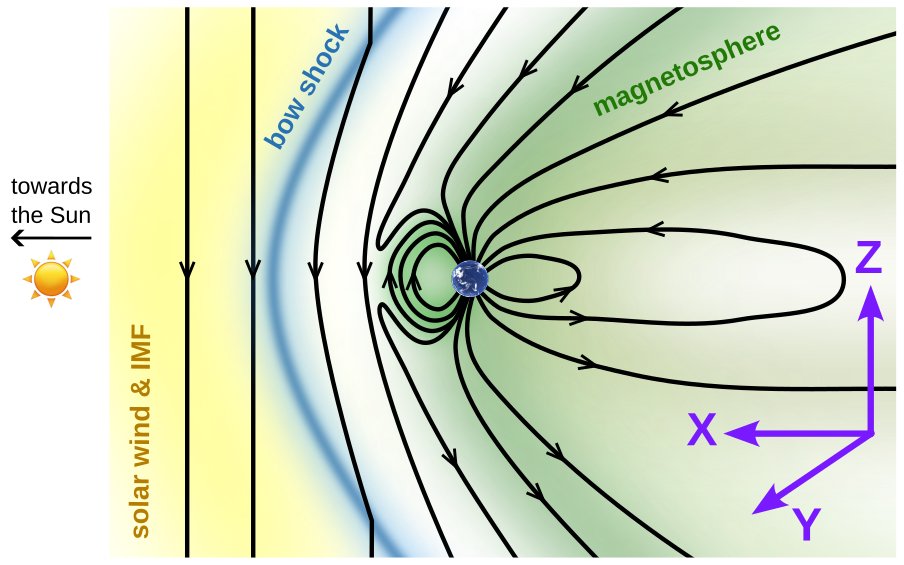
\includegraphics[width=\linewidth]{Fig6_GSE_IMF.png}
  \caption{Diagram illustrating the GSM coordinate system often used to express the IMF components. When the IMF points towards the south (negative Bz) like in this figure, magnetic reconnection takes place at the dayside magnetosphere. Image credit: Maxime Grandin.}
  \label{fig-bz}
\end{figure}

The Sun's expanding atmosphere, called the solar corona, has a magnetic field which is carried along with the solar wind towards the outskirts of the solar system. This forms what is known as the interplanetary magnetic field (IMF). At every given moment, invisible field lines are stretching and flowing around our planet, usually buffeted away by its own protective magnetic shield.

Magnetic fields can be considered vectors in 3D space. That means in order to fully describe the orientation and magnitude of the IMF, one needs to consider its components along three directions forming a coordinate system which can be used to describe the three-dimensional world we live in. For practical purposes, we often consider the IMF in a reference frame called the Geocentric Solar Magnetospheric (GSM) system. In the GSM system, the X axis points towards the Sun, the Z axis is aligned with the Earth's magnetic dipole, and the Y axis completes the system (roughly pointing towards dusk). This is illustrated in Figure~\ref{fig-bz}. We then talk about the Bx, By and Bz components of the IMF.

When the IMF has its Z-component pointing south (i.e. Bz is negative), it is able to ``couple'' with Earth's magnetic field, and both energy and particles from the solar wind can then transfer through Earth's magnetic shield. This process is known as \textbf{magnetic reconnection}. Why Bz south? Without delving into complicated details, this comes from the fact that Earth's magnetic field points north, as illustrated in Figure~\ref{fig-bz}. Hence, when southward IMF reaches the dayside magnetosphere, this brings two oppositely directed magnetic fields close to each other. Such conditions are known to favour magnetic reconnection, which leads to field lines ``snapping together'' and producing what is called ``open field lines'' in space physics. Open field lines have one end connected to Earth and the other extends out into the solar wind, ultimately reaching the Sun. This is in contrast to 'closed' magnetic field lines, which have both ends connected to Earth, one in the northern and the other in the southern hemisphere. When magnetic reconnection happens on Earth's dayside, magnetic field lines are changed from 'closed' to 'open' and energy is transferred from the solar wind to the magnetosphere.

The open field lines are then carried towards the nightside of the Earth due to the anti-Sunward motion of the solar wind, where they accumulate. Adding new magnetic field lines to the magnetotail causes a pressure that pushes field lines together there. Since the field lines are once again pointing in opposite directions to each other in the magnetotail, this eventually causes magnetic reconnection on the nightside. When this happens, charged particles (electrons and protons) stream back to Earth following the newly closed magnetic field lines, and they reach the upper atmosphere within the auroral oval. These are the ``precipitating particles'' mentioned in Section~\ref{what-is-aurora}. When a major reconnection event takes place in the magnetotail, we get a substorm (see~\ref{auroral-substorms}).

This is why when the IMF Bz points south, this usually correlates with an increased chance of aurora. The full process (dayside and nightside reconnection) is known as the Dungey cycle. The reconnection between the IMF and Earth's magnetic field on the dayside of the Earth can produce aurora during the daytime hours (dayside aurora, visible during the polar night in few locations such as Svalbard). On the other hand, the nightside aurora is associated with reconnection in the magnetotail and substorms.

The physics of substorms, magnetic reconnection, and solar wind--magnetosphere--ionosphere coupling could fill an entirely separate handbook, but here are some general tips for aurora chasers for watching the IMF Bz:
\begin{enumerate}
    \item The further south the Bz is, the generally better conditions there are for aurora.
    \item The longer that Bz remains pointing south, the more enhanced aurora will become.
    \item Typically, Bz south conditions persisting for more than a few hours will cause the aurora to be enhanced.
    \item Strong changes in the Bz (i.e. a sharp turning from southwards to northward) can sometimes cause substorms.
\end{enumerate}

While not mentioned in this section, Bz is not the only solar wind parameter worth monitoring. Bt, or the total field strength, is also important along with solar wind speed and density.

\subsubsection{Real-time Online Updates}
If you are at any point confused or overwhelmed with the apparent complexity of aurora science used to inform when to go out, ground-truth information in the form of aurora reports is still better than interpreting forecasts or proxy data (e.g. solar wind). The best practice is to find an aurora chasing community on Facebook, X, Instagram, etc. that is specific to your area and stay aware of when members start reporting aurora sightings. \href{https://www.aurorasaurus.org}{Aurorasaurus}\footnote{https://www.aurorasaurus.org} \cite{MacDonald2015} is a platform where aurora chasers can report sightings in real-time. When clusters of positive sightings are made, aurora alerts are sent out to users in that local area. More information regarding Aurorasaurus can be found in Section \ref{aurorasaurus}.

Mobile and desktop applications are a great way to monitor auroral activity at-a-glance. While there are many aurora apps currently available, \href{https://spaceweatherlive.com/}{SpaceWeatherLive}\footnote{https://spaceweatherlive.com/} and \href{https://aurora-alerts.uk/}{Glendale Aurora}\footnote{https://aurora-alerts.uk/} are reputable apps supported by dedicated owners/development teams. Popular enthusiast websites for monitoring solar and geomagnetic activity and space weather events are \href{https://www.solarham.net/}{SolarHam}\footnote{https://www.solarham.net/}, \href{https://spaceweather.com/}{spaceweather.com}\footnote{https://spaceweather.com/}, and \href{https://www.thesuntoday.org/}{thesuntoday.org}\footnote{https://www.thesuntoday.org/}.

For more information on space weather predictions and realtime observations, consult official sources from space weather offices like \href{https://www.swpc.noaa.gov}{NOAA Space Weather Prediction Center}\footnote{https://www.swpc.noaa.gov} and \href{https://www.sidc.be}{Solar Influences Data Analysis Center's Space Weather Services}\footnote{https://www.sidc.be} and local aurora chasing groups on social media.

\section{Auroral Research \& Citizen Science Highlights}
\index{citizen scientist!contributions}
This section shows some highlights of citizen scientists' contributions to auroral research. Specifically, the section describes STEVE and SAR arcs, dunes, fragments, continuum emissions, and proton aurora.


\subsection{STEVE \& SAR Arcs}\label{steve-sar-arcs}\index{STEVE!discovery}  
%\contributed{Bea, Carlos}
STEVE is the name given to a white-mauve ribbon stretching across the night sky along the east--west direction and that is generally seen during the recovery phase of a substorm at subauroral latitudes (i.e. latitudes equatorwards of the auroral oval). An example of STEVE is shown in Figure~\ref{fig-stevesararc} (top).

The first significant discussion about STEVE in the scientific community occurred on 15~January 2016, when Dr~Elizabeth MacDonald gave a talk at the University of Calgary, drawing perhaps the largest crowd in some time to the Physics and Astronomy Department's Friday afternoon colloquium. The host, Dr~Eric Donovan, noted the attendance of many unfamiliar faces. Dr~MacDonald was well-known in the area for her successful project, Aurorasaurus. After her talk, citizen scientists from the Facebook group Alberta Aurora Chasers began sharing numerous images of an unusual auroral structure. Neither MacDonald nor Donovan, despite their extensive knowledge, had ever seen anything like it. They encouraged the citizen scientists to choose a placeholder name without physical connotations. Inspired by the movie Over the Hedge, Chris Ratzlaff suggested the name STEVE. This later became a backronym defined by Prof. Robert Lysak from the University of Minnesota, standing for Strong Thermal Emission Velocity Enhancement \cite{Gallardolacourt_2019}.

In recent years, the collaboration between the scientific community and citizen scientists has been crucial in advancing our understanding of STEVE and the associated processes, and research has intensified. The scientific community now understands that STEVE is not produced by particle precipitation. Instead, it is associated with extremely fast subauroral (equatorwards of the auroral oval) plasma flows that provide the energy for the emission. STEVE typically occurs after auroral activity. However, many questions remain, such as the mechanisms responsible for and relationship between STEVE and other features that appear nearby such as the ``picket fence'' and ``streaks''.

The typical {\bf characteristics of STEVE} in the night sky are:

\begin{itemize}
\item {\bf Colour and Shape}: White-mauve arc or ribbon. 
\item {\bf Brightness}: As bright as the aurora and therefore visible with the naked eye.
\item {\bf Location}: Always equatorwards of the auroral oval. 
\item {\bf Size}: Typically very narrow in latitude (north to south), but extends over several thousands of kilometres in longitude (east to west).
\item {\bf Duration and Stability}: Lifetime of about an hour or less with varying stability.
\item {\bf Other Helpful Information}: STEVE is typically observed after a substorm. Sometimes, STEVE is accompanied by a set of green, finger-like, vertical structures known as the ``picket fence''. Small features aligned almost at right angles to the picket fence also sometimes appear, which are called ``streaks'' \cite{Semeter2020}.
\end{itemize}

\begin{figure}[h!]
  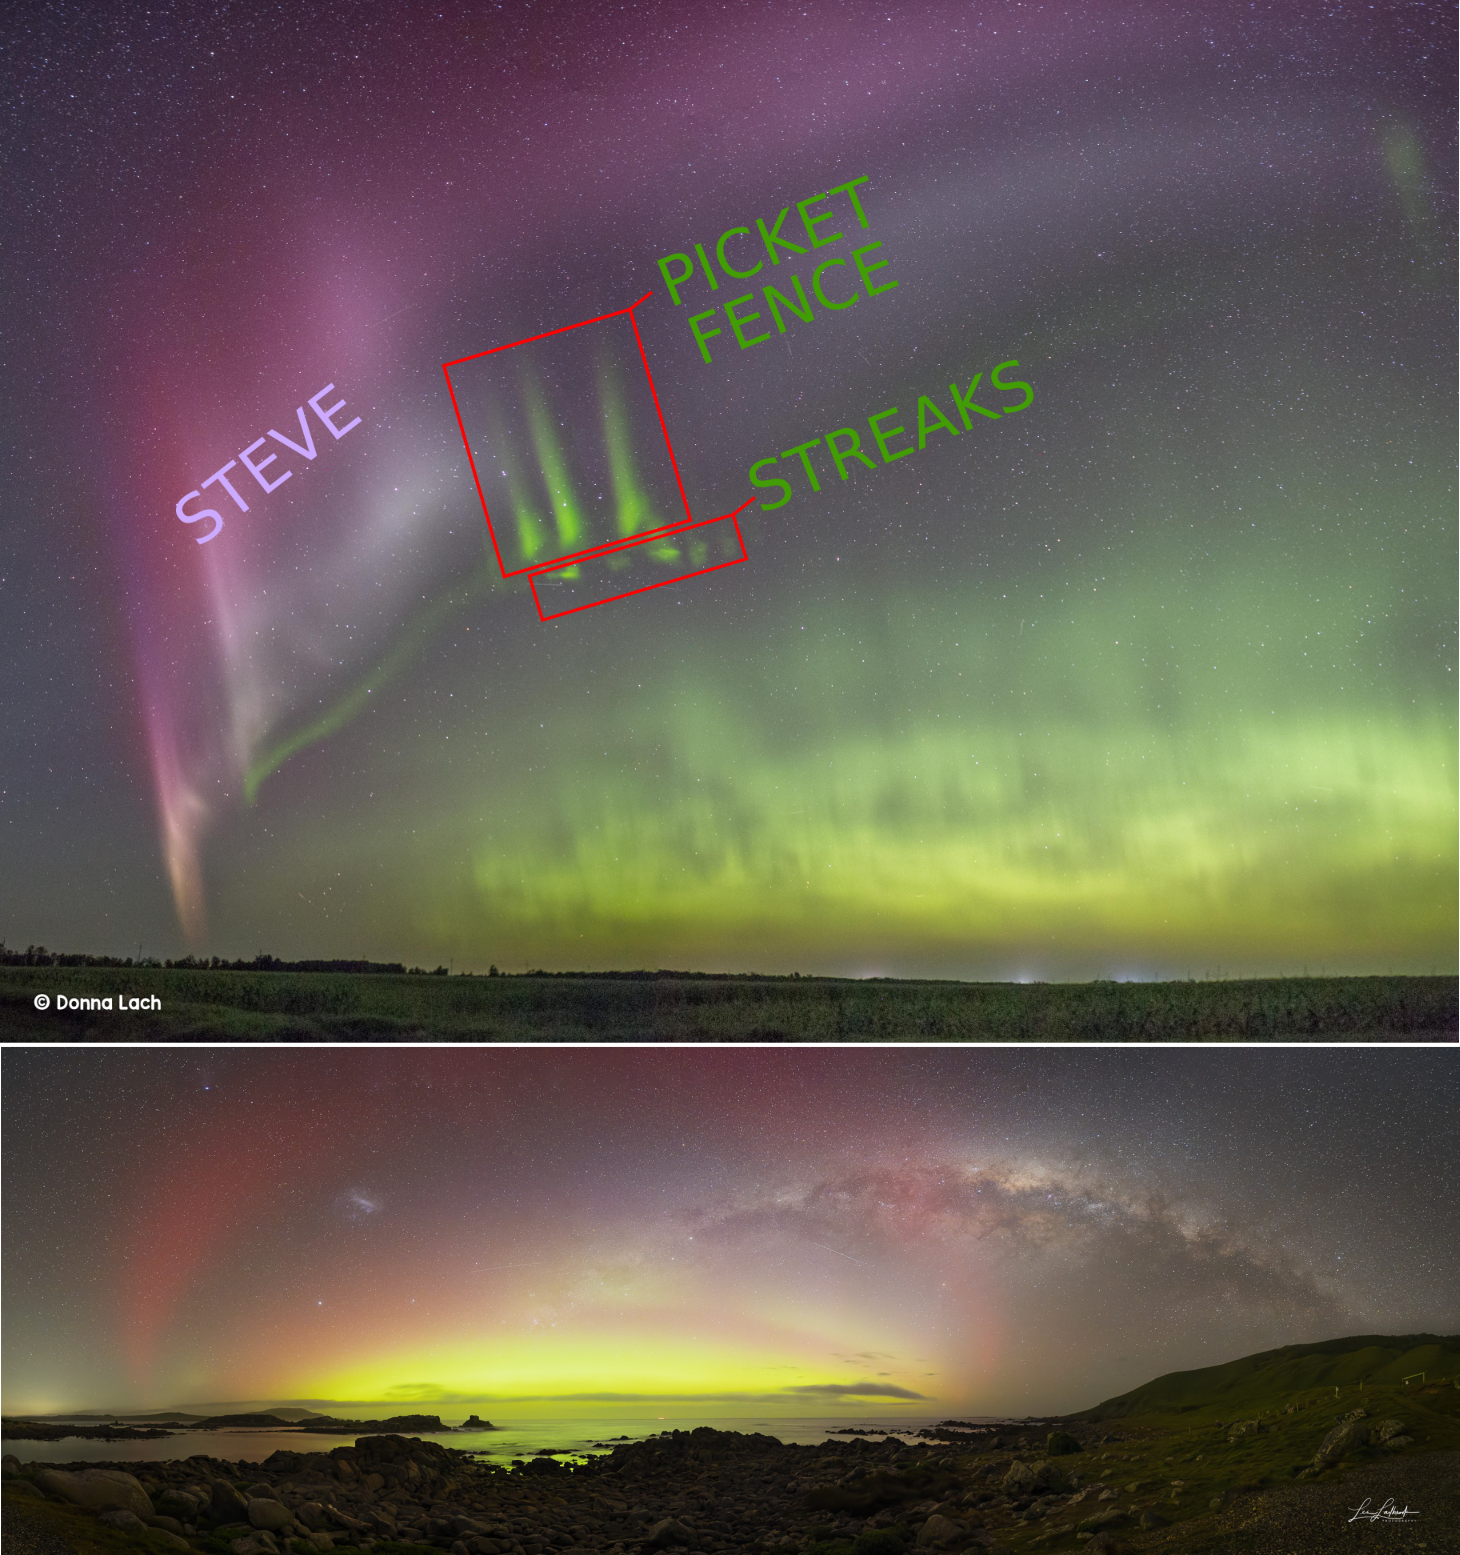
\includegraphics[width=\linewidth]{Fig7_stevesararc.png}
  \caption{Top: Thin mauve STEVE arc with picket fence and streaks photographed by Donna Lach. Bottom: Thick diffuse SAR arc photographed by Les Ladbrook.}
  \label{fig-stevesararc}
\end{figure}
In the same region where STEVE is observed, another optical phenomenon known as the Stable Auroral Red (SAR) arc has been studied for decades \cite{Kozyra1997, Mendillo_2016a, Martinis2022}. An example of SAR arc is shown in Figure~\ref{fig-stevesararc} (bottom). While SAR arcs differ from STEVE in terms of optical characteristics, duration, and latitudinal extent, they also share some similarities, such as their location and wide longitudinal extent. Recent observations by scientific instruments and citizen scientists have documented temporal transitions between STEVE and SAR arcs. This line of research has raised numerous questions about the dynamics of the subauroral ionosphere and how it changes rapidly in short time periods.\\

SAR arcs are characterised by faint red line emission only and are generally not observable with the naked eye. However, recent studies have reported instances of extremely bright SAR arcs during transitions between STEVE and SAR arcs \cite{Martinis2022}. Some typical {\bf characteristics of SAR} arcs include:

\begin{itemize}
\item {\bf Colour and Shape}: A diffuse red arc.
\item {\bf Brightness}: Typically dim and not visible with the naked eye.
\item {\bf Location}: Like STEVE, SAR arcs are always observed equatorwards of the auroral oval, near a region with decreased electron density.
\item {\bf Size}: Broader than STEVE (hundreds of kilometres), but also extending widely from east to west. In occasions, SAR arcs have been observed to cover the entire globe \cite{Mendillo2013}.
\item {\bf Duration and Stability}: SAR arcs can last up to many hours. The spatial characteristics remain relatively unchanged, although evidence exists showing variability and dynamical changes \cite{Mendillo_2016a}.
\item {\bf Other Helpful Information}: SAR arcs are diffuse and do not have rays. SAR arcs have been observed alongside multiple green emission features, probably related to low-energy electron precipitation \cite{Mendillo_2016a}.
\end{itemize}

\subsection{Dunes}\label{dunes}\index{dunes!discovery}  
%\contributed{Emma, Maxime}
Dunes, or dune aurora, is a type of night sky emission consisting of diffuse green light exhibiting a wave-like field of parallel structures. It is generally a dim auroral form, barely distinguishable with the naked eye and best identified in pictures. Example photographs of dunes are shown in Figure~\ref{fig-duneexample}; these images have been processed to enhance contrasts between the brighter and dimmer structures.

The first dune event that sparked widespread public discussion among aurora observers in Finland occurred during the geomagnetic storm on 7~October 2015. The conversation concerning the explanation of the presence of wave-like structures in the diffuse aurora began on Skywarden and continued in the Revontulikyttääjät Facebook group (translated as ``Aurora Stalkers''), which as of October 2024 consists of 41,000~aurora chasers, primarily from Finland. The mystery remained unsolved, until the image material was presented to Prof.~Minna Palmroth from the University of Helsinki in 2018. Palmroth was intrigued and could not relate the dunes to any known auroral form described in the peer-reviewed scientific literature at that time. Conveniently, the dunes reappeared on 7~October 2018 (exactly three years after the event mentioned above) and were photographed by several observers in southern and central Finland, which provided an excellent chance to investigate them in more detail. The two pictures shown in Figure~\ref{fig-duneexample} are from that event and were published in a scientific paper by \textcite{Palmroth2020}. In this study, using a triangulation method based on the two simultaneous pictures, Dr~Maxime Grandin determined that the altitude at which the dunes were present was close to 100~km. 

A subsequent collaboration on a dune event which occurred on 20~January 2016 took place between between scientists and six citizen scientists from three different European countries: Finland, Norway, and Scotland. This second study revealed that some dune events can be seen over a very wide area and can persist for several hours: the largest-scale dune event investigated so far covered an area spanning over 1500~km in the east--west direction and lasted for at least four hours \cite{Grandin2021}.
\begin{figure}[h!]
  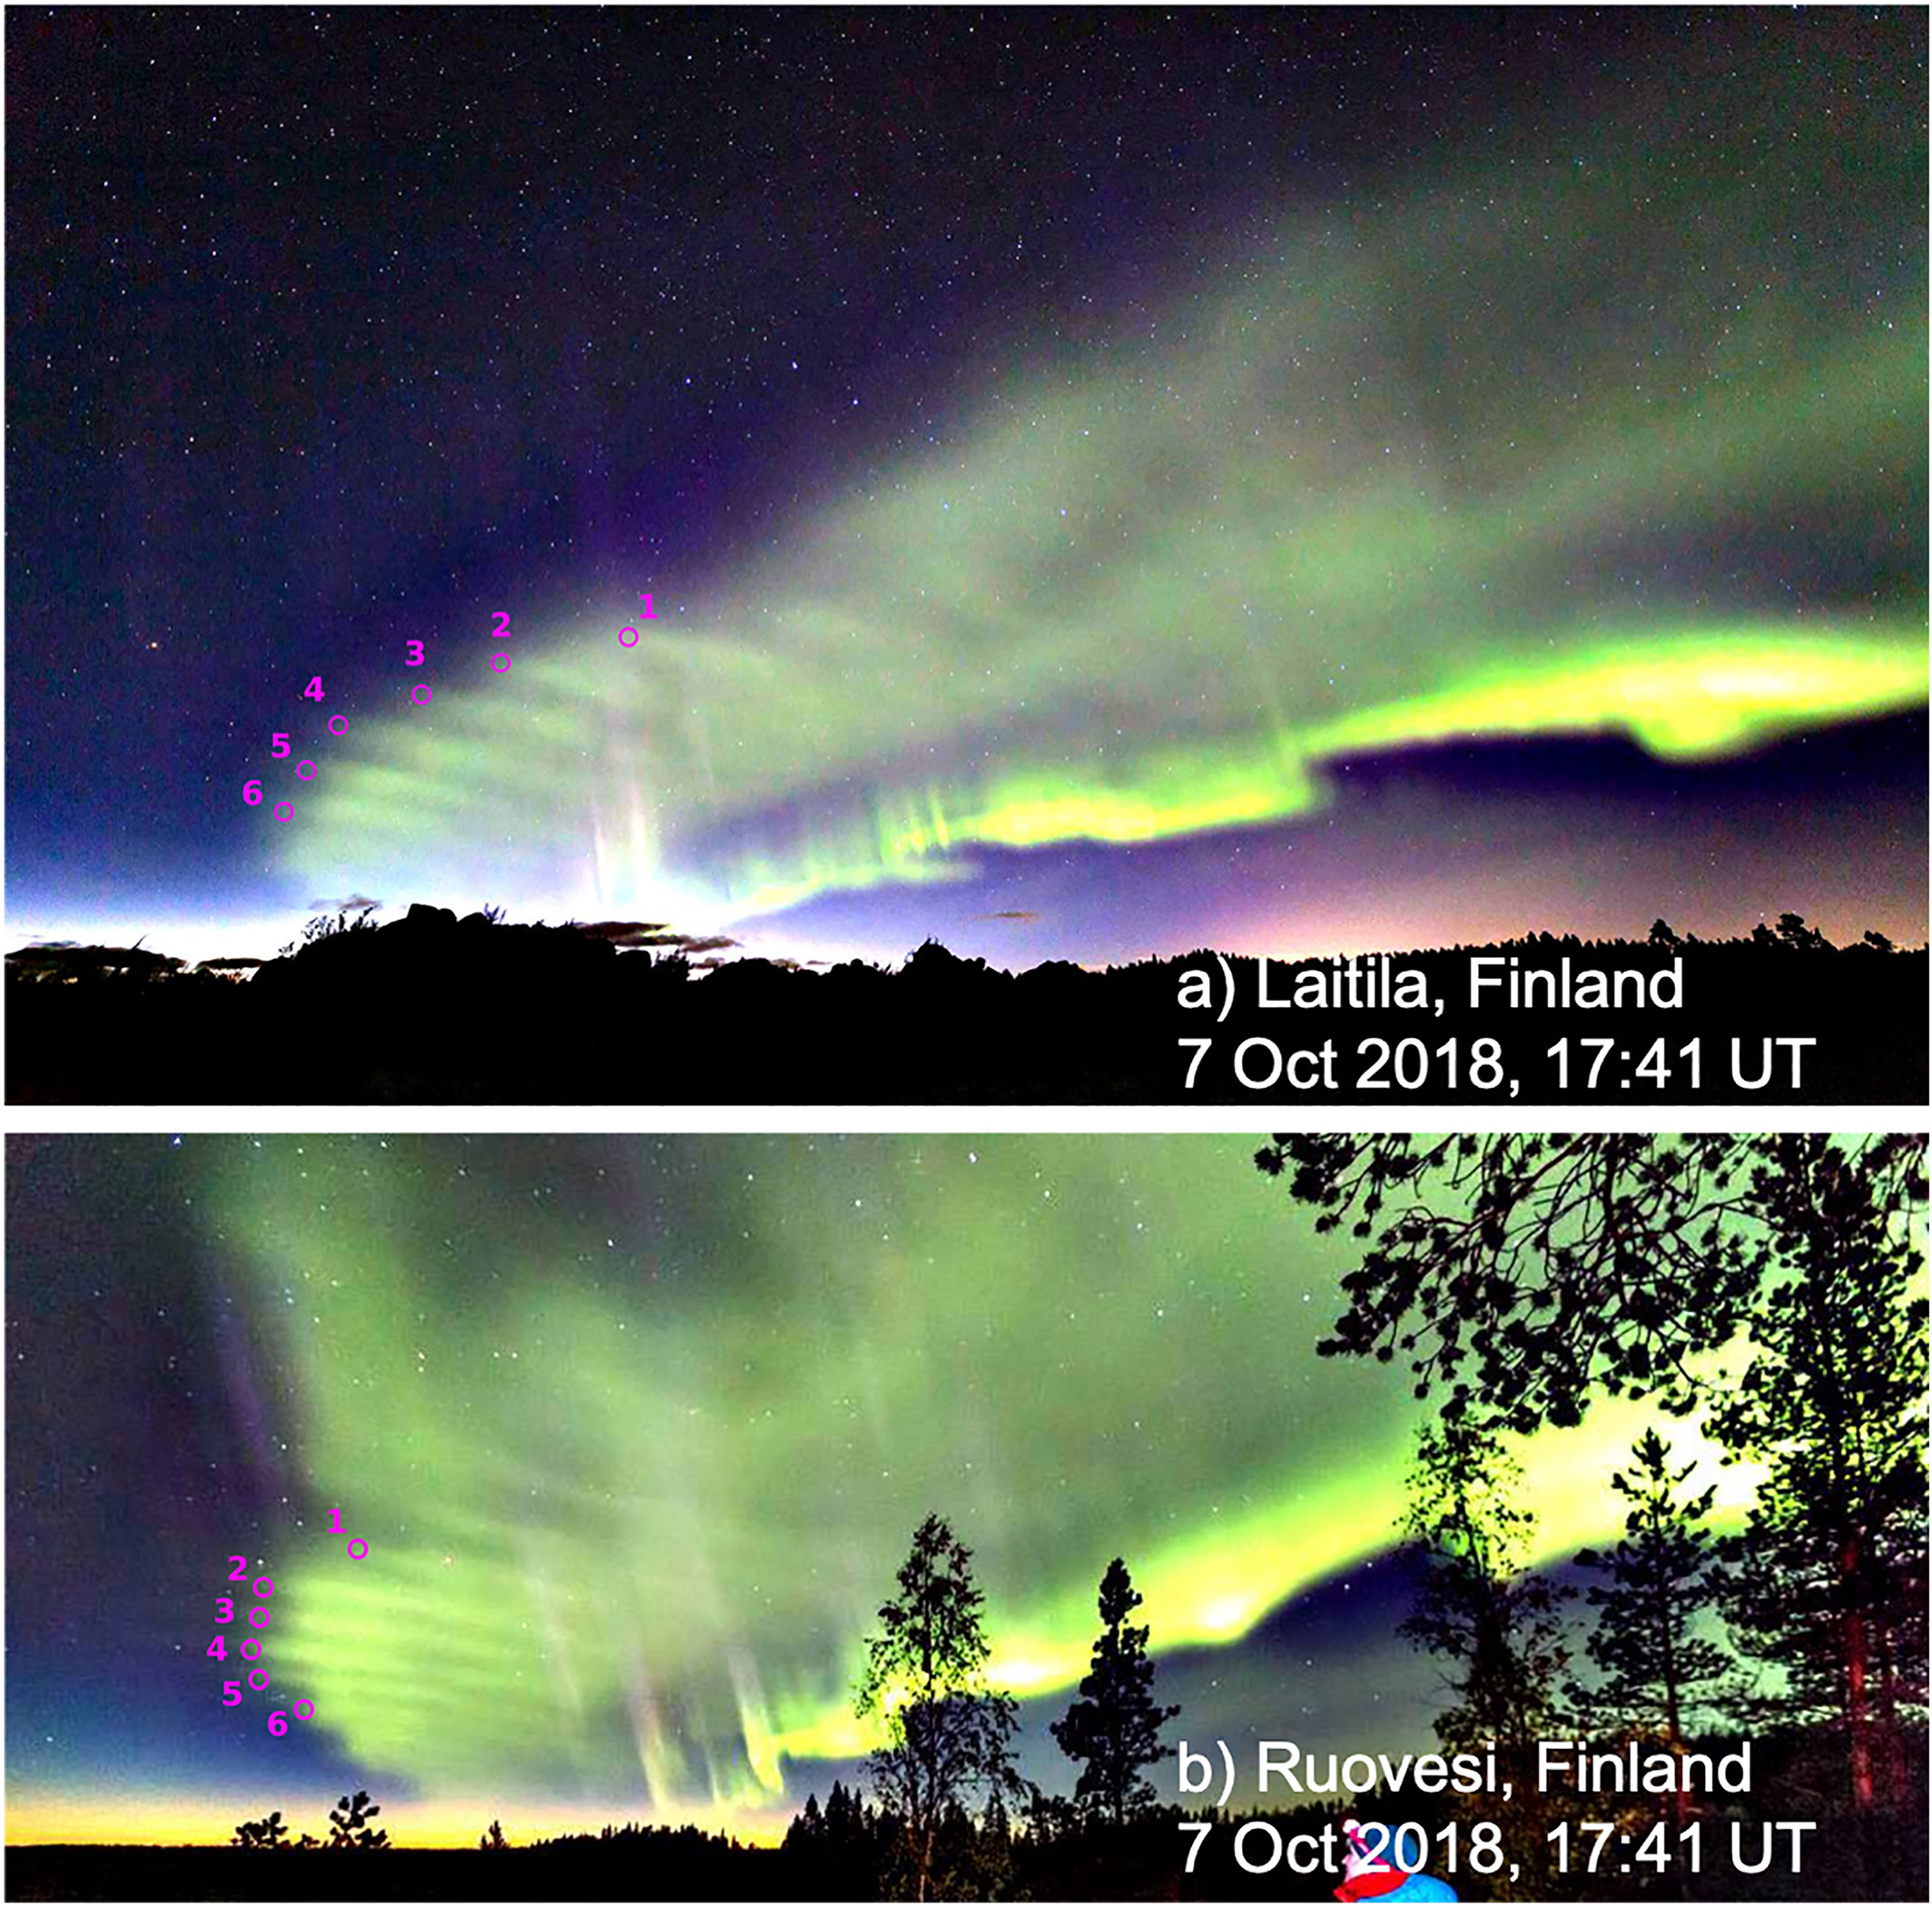
\includegraphics[width=\linewidth]{Fig8_dunes.jpg}
  \caption{Citizen scientist observations of dunes presented in \textcite{Palmroth2020}. The top picture was taken by Pirjo Koski and the bottom picture by Rami Valonen.}
  \label{fig-duneexample}
\end{figure}

Some typical {\bf characteristics of dunes} can be summarised as follows:
\begin{itemize}
    \item \textbf{Colour and Shape:} Green parallel finger-like structures embedded within green diffuse aurora.
    \item \textbf{Brightness:} Too dim to be spotted with naked eye, although sometimes they can be distinguished if knowing that they are present (e.g. if visible in pictures).
    \item \textbf{Location:} In most of the known cases, the dunes are close to the equatorward edge of the auroral oval.
    \item \textbf{Size:} Large scale and the region of dunes can span over 1500 km in the east--west direction.
    \item \textbf{Duration and Stability:} Can last for hours and drift slowly. 
    \item \textbf{Other Helpful Information:} Dunes are relatively rare and typically observed only a few times each year, most often between October and January. It is important to verify that the patterns seen in photos are not simply diffuse aurora partially obscured by cloud layers forming parallel bands.
    \end{itemize}

The current understanding of the dunes suggests that they are caused by a large-scale atmospheric wave, likely a rare ``mesospheric bore'', which forms at the boundary between the mesosphere and thermosphere. This wave alters the atomic oxygen concentration, creating alternating dense and void bands. When diffuse aurora is present, this results in parallel brighter and dimmer bands, with the atmospheric wave’s horizontal movement explaining the dunes' drift.

While the mesospheric bore is the primary suspect, other waves, like atmospheric gravity waves, may also produce similar auroral patterns. The diffuse green layer at the oval's equatorward edge, called the ``dune shelf'' by Finnish citizen scientists, can appear with or without dunes, depending on the presence of atmospheric waves. Occasionally, another wavy structure called a ``giant undulation'' may be seen at the edge of the dune shelf.

\subsection{Fragments}\label{fragments}
%\contributed{Katie}
\begin{figure}
  \includegraphics[width=\linewidth]{Fig9_Fragments_SophieCordon.png}
  \caption{Image of aurora over Svalbard where a chain of fragments is indicated by a red arrow. Image credit: Sophie Cordon.}
  \label{fig-fragmentsexample}
\end{figure}

A strange type of aurora-like feature was spotted over Svalbard (Norway) and first recorded in two scientific papers in 2021 \cite{Dreyer2021, Whiter2021}. Citizen scientists contributed to the early work on fragments by classifying one of the events used in \textcite{Whiter2021}, using the online project Aurora Zoo (see \ref{classification}).\index{citizen scientist!contributions} The features were named Fragmented Aurora-like Emissions (FAE) or simply ``fragments''. They appear as small bits of green light and typically last for under a minute. They can, but do not always, appear close to auroral arcs and they can appear alone or in chains of multiple fragments next to each other. An example of a chain of fragments taken by photographer and citizen scientist Sophie Cordon can be seen in Figure~\ref{fig-fragmentsexample}. Just because the fragments were first written about in scientific papers in 2021 does not mean that photographers do not have photos of the phenomena on their hard drives from many years previously, which Sophie proved by providing many examples of fragments from 2015--2023.  After the features were first named in 2021, awareness grew in the auroral photography community and citizen scientists began identifying fragments in their images. As of October 2024, scientists are aware of observations from only a handful of locations: Svalbard, Northern Norway and Northern Finland, Greenland, Iceland, Canada, and Antarctica. There are a low number of observations in locations other than Svalbard. For advice on the camera settings recommended for capturing fragments, see \ref{short-lived-transient-features}.

Some typical {\bf characteristics of fragments} can be summarised as follows:
\begin{itemize}
    \item \textbf{Colour and Shape:} Green, small features that form at right angles to the magnetic field. They appear alone or in a chain. 
    \item \textbf{Brightness:} During strong auroral displays fragments are as bright as the surrounding aurora so are easier to observe. During low activity, with little or no aurora, the fragments are also dimmer and not possible to see without a camera.
    \item \textbf{Location:} Fragments have so far mostly been observed at the northernmost edge of the auroral oval but new observations suggest that they can occur within the auroral oval itself. Perhaps it is harder to see the fragments within the oval due to other bright aurora hiding them. 
    \item \textbf{Size:} Small scale (few kilometres).
    \item \textbf{Duration and Stability:} Individual fragments last from seconds to minutes and show a drifting motion. If the fragments happen, it is likely that they may happen again soon after since the conditions that cause them might persist. 
    \item \textbf{Other Helpful Information:} Fragments look a lot like the streaks that are seen at the base of STEVE and the picket fence\index{picket fence} (see \ref{steve-sar-arcs})\index{STEVE}. Fragments and streaks occur in different locations with respect to the auroral oval and appear alongside different auroral features. Fragments have been seen alone or close to auroral arcs just polewards of or within the auroral oval, while streaks have mainly been seen with STEVE and the picket fence equatorwards of the auroral oval. 
    \end{itemize}
 
Both fragments and streaks are special as they point in a direction almost at right angles to the magnetic field line. This is strange because aurora is caused by particles moving along the magnetic field direction, so auroral emissions are usually directed up and down the magnetic field line direction. Researchers think that fragments and streaks are not caused by particles flowing down the magnetic field lines but may be caused by a yet-to-be identified process in the ionosphere. What causes the fragments is currently unknown, although researchers have suggested some theories, including the Farley-Buneman instability. Confirming whether the fragments are caused by the suggested mechanisms is a high priority for the researchers. 



\subsection{Continuum Emissions}\label{continuum}\index{continuum!discovery} 
%\contributed{Rowan, Noora}
\begin{figure}[h!]
\begin{centering}
  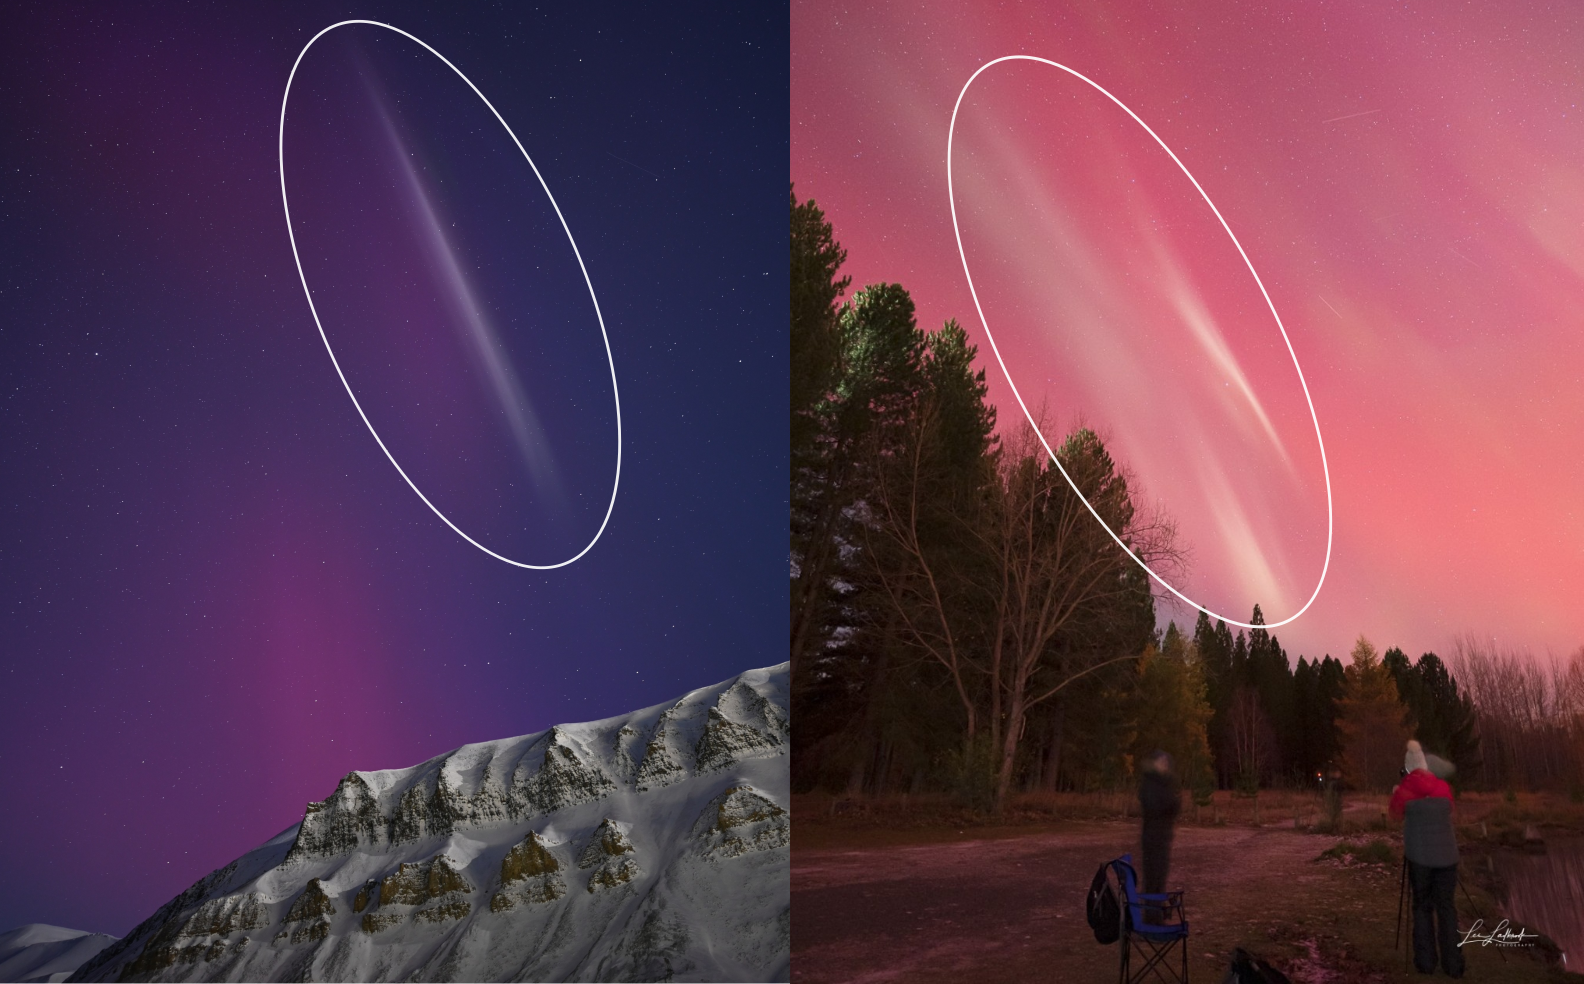
\includegraphics[width=\linewidth]{Fig10_Continuum.png}
  \caption{(Left) Image of aurora over Svalbard with faint red emission background and a thin white-ish stripe of continuum emission that is aligned with the magnetic field direction. Image credit: Marjan Spijkers. (Right) Image over New Zealand showing stripes of white-itsh continuum emission with a pink/red background. Image credit: Les Ladbrook.}
  \label{fig-continuumexample}
  \end{centering}
\end{figure}

Continuum emissions have been recognised for decades, but recently, the mauve/grey/white emissions have attracted renewed interest in relation to STEVE \cite{Gillies2019}. These emissions and made up of all the different colours in the visible wavelength range, which combine together to appear off-white. They have been identified as characteristic of STEVE, primarily occurring at the equatorward edge of the auroral oval. However, observations in 2024 from Tromsø \cite{Nanjo2024} indicate that STEVE-like conditions may also exist polewards of the green aurora. Both types of continuum emissions typically manifest as thin arcs of pale light. These emissions have been observed within dynamic aurora and at the poleward edge of the auroral oval, and they are seen to change in brightness and shape in step with the nearby aurora that is created by particle precipitation. The precipitation-induced continuum emission structures can take on various shapes and evolve rapidly, similar to dynamic aurora. Examples of continuum emissions are shown in Figure~\ref{fig-continuumexample}.

Some typical {\bf characteristics of continuum emissions} can be summarised as follows:
\begin{itemize}
    \item \textbf{Colour and Shape:} Pale mauve/grey/white colour. They can appear as thin or wide arcs or more rayed structures.
    \item \textbf{Brightness:} Variable.
    \item \textbf{Location:} Polewards, within, and equatorwards of the auroral oval. Continuum emissions have also been seen at high latitudes in the dayside aurora, so they are not necessarily a nightside feature like STEVE.
    \item \textbf{Size:} Variable. They can be fine scale ray-like features, thin ribbons like STEVE, or thick arcs.
    \item \textbf{Duration and Stability:} Variable. The thinner, more dynamic emissions typically last seconds to minutes, while the arc-like features can last hours.
    \item \textbf{Other Helpful Information:} It is worth noting that the colour of the continuum emission in colour images depends on the background illumination of the sky, including the aurora. There are therefore different shades of pale.
    \end{itemize}


The actual generation mechanism for continuum emissions is not known, but it is likely that ionospheric heating by particle precipitation and/or strong plasma flows play an important role. The variety of different conditions where continuum emissions occur suggests that a combination of different mechanisms might work together to produce a favourable environment.

The only bullet-proof evidence of continuum emission is a scientific measurement showing the brightness over a range of measured wavelengths. However, many photos provide relatively convincing observations even without these measurements. 


\subsection{Proton Aurora}\label{proton-aurora}\index{proton aurora}
%\contributed{Rowan, Eero}

Most proton precipitation (protons raining into the Earth's atmosphere from near-Earth space) results in proton aurora, which is diffuse and invisible to the naked eye. Sometimes protons may also contribute to weak visual emission by releasing enough ``secondary electrons''. A secondary electron is taken off an atmospheric atom or molecule when a precipitating proton carries enough energy to ionise it. This electron then follows the magnetic field direction downwards and can excite atmospheric constituents in the same way as a precipitating particle coming from space, leading to auroral emissions. The auroral structures associated with secondary electrons are sometimes called proton blobs, proton patches, or isolated proton arcs. They  appear equatorwards of the main auroral oval, often around dusk, and typically show up as green emissions that are separate from the main oval.

During 2015--2022, Finnish and Canadian citizen scientists documented several events of isolated, green proton structures with a faint red arc above the proton blob structure. Both the red arc and the green aurora were aligned with the emissions happening at different altitudes: red at about 230 km height and green at about 110 km \cite{Nishimura2022}. This combination of the red and green proton aurora is called Red Arc with Green Diffuse Aurora (RAGDA). An example of this scene is shown in Figure~\ref{fig-ragdaexample}.


\begin{figure}[h!]
  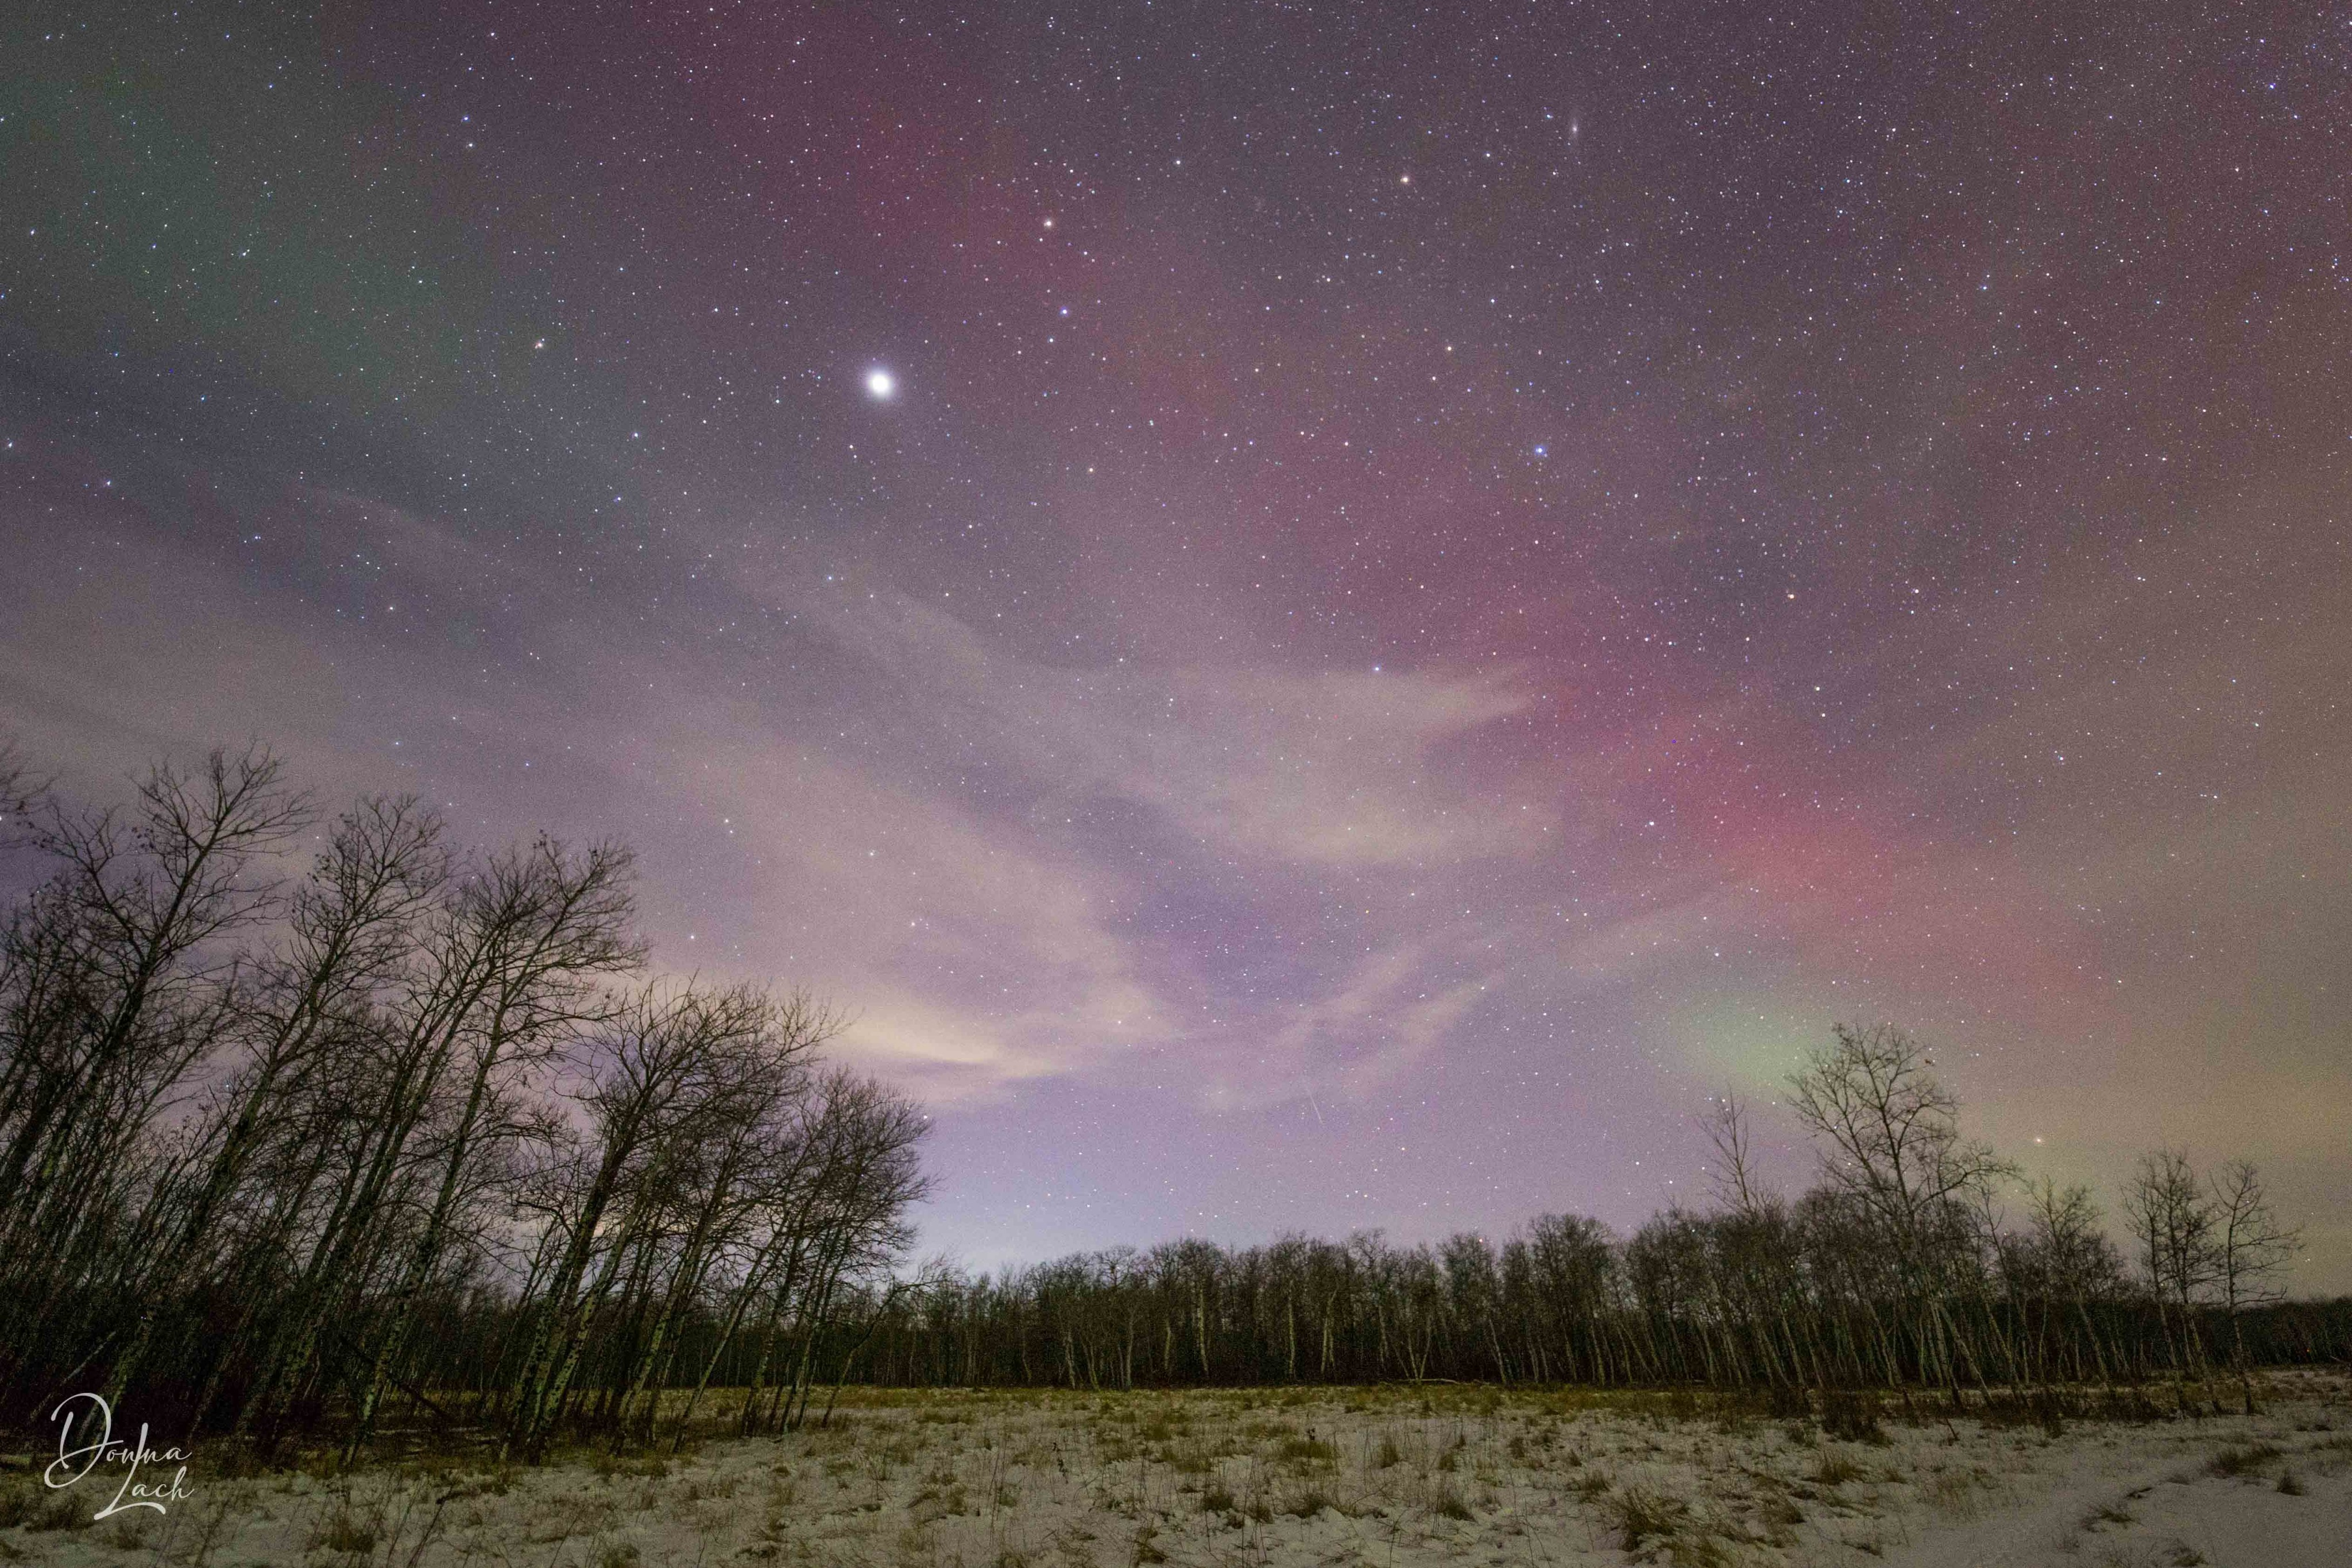
\includegraphics[width=0.9\linewidth]{Fig11_RAGDA_DonnaLach.jpg}
  \caption{Diffuse emissions of red and green close by form RAGDA in the subauroral latitudes. Image credit: Donna Lach.}
  \label{fig-ragdaexample}
\end{figure}

Although the red arc in RAGDA is not a SAR arc (see \ref{steve-sar-arcs}), sometimes proton precipitation can trigger a SAR arc or leave one behind after the proton activity fades out. During this transition, distinguishing between the different arcs based on their cause can be visually challenging. 

Some typical {\bf characteristics of proton aurora} can be summarised as follows:
\begin{itemize}
    \item \textbf{Colour and Shape:} Red or green diffuse aurora in arcs or blobs.
    \item \textbf{Brightness:} Dim.
    \item \textbf{Location:} Equatorwards of the auroral oval.
    \item \textbf{Size:} Variable but arcs can be elongated over thousands of kilometres.
    \item \textbf{Duration and Stability:} RAGDA can typically last for tens of minutes to hours but the proton blobs have shorter lifetimes.
    \item \textbf{Other Helpful Information:} A useful guideline is that only RAGDA displays diffuse rayed structures in the red arc, and SAR arcs lack the diffuse green emission blobs seen beneath RAGDA.  
    \end{itemize}

\subsection{Open Questions in Aurora Science}\index{aurora!open questions}

It is commonly assumed that scientists already know everything there is to know about the aurora, but that is far from true. In fact, there are many unresolved questions in auroral science. Researchers are still trying to understand the energy processes behind the aurora and how different auroral shapes and behaviours form. Citizen scientists, through their observations and photos, can play a crucial role in helping scientists answer these open questions in the future.

Some key open questions about auroral emissions include:
\begin{itemize}
    \item What causes subauroral emissions like \textbf{STEVE}, the \textbf{picket fence}, and \textbf{SAR arcs}?
    \item What mechanisms produce small-scale auroral features like \textbf{fragments} and \textbf{streaks}?
    \item What creates \textbf{continuum emissions}?
\end{itemize}

In addition to these, specific auroral forms raise even more questions:
\begin{itemize}
    \item What is the connection between \textbf{STEVE} and the \textbf{picket fence}, and why is the picket fence sometimes present but not always?
    \item What are all the different auroral forms, and is there a pattern to how they change from one shape to another?
    \item How do \textbf{STEVE} and \textbf{SAR arcs} interact?
    \item What kind of atmospheric waves produce the \textbf{dunes}, and are they caused by auroral activity or do they exist beforehand?
    \item What causes the spectacular \textbf{red aurora} during some storms?
\end{itemize}

Finally, the interaction between the \textbf{magnetosphere} and the \textbf{ionosphere} is a particularly active area of research, with questions like:
\begin{itemize}
    \item How can we learn to better predict auroral substorms and what triggers them?
    \item How does the magnetosphere contribute to \textbf{STEVE and continuum emissions}?
    \item How are the different shapes and patterns of the aurora connected to changes in the magnetosphere over time?
    \item How exactly are particles accelerated in the auroral region?

    
\end{itemize}

\section{How to Take an Aurora Photo}\index{photography}\index{aurora chasing} 
This section outlines the essential equipment for capturing aurora photos, recommended camera settings, fundamental image processing techniques, and tips from experienced aurora photographers. It provides an introduction to aurora photography, while Section~\ref{imaging-for-science} expands on these basics, focusing on how to capture aurora images suitable for scientific research.


\subsection{Equipment}\index{photography}\index{equipment}
%\contributed{Chris, Vincent, Donna}

You do not need fancy equipment to capture stunning photos of the aurora. Whether you have a high-end camera or just your smartphone, you can still take beautiful shots. A lack of expensive gear is not a barrier to enjoying and photographing the aurora. However, if you are passionate about aurora photography and considering investing in some equipment, here are some explanations that will help and some features that are beneficial for capturing aurora for research.

\subsubsection{Camera Features / Types}\index{equipment!cameras}\index{equipment!mobile phones}

\begin{itemize}
\item \textbf{Internal GPS:} This is the best way to ensure you have your location pinpointed in order for the scientists to triangulate the auroral feature or find satellite data relative to the observation. Some internal GPSs can wear down your battery faster. An external GPS can be connected but is cumbersome. 

\item \textbf{Intervalometer:} This could be a permanent feature or downloaded as an app to the camera. It is important for timelapse photography. An external intervalometer can be connected but is cumbersome.

\item \textbf{Video:} If you are regularly under the auroral oval, you will have a lot of opportunities to take aurora video which is very helpful to study the fine-scale structures of the aurora. Mirrorless cameras like the Sony A7s III and Canon R6 take smaller photos and are more efficient for taking videos.

\item \textbf{Colour:} Each brand seems to capture colours a little differently, but as new cameras emerge the difference becomes less. Something to note is that a Sony can capture brilliant greens. 

\item \textbf{Full Frame vs Cropped Frame:} To capture more of the sky and everything you see through the camera, full frame is optimal but not necessary to get an aurora photo.

\item \textbf{Mirrorless:} The cutting edge of camera technology is the mirrorless camera. They are usually lighter, more compact, and shoot faster. However, you will likely go through more batteries in a night with a mirrorless camera than with a DSLR and some mirrorless cameras can have limited lens options.

\item \textbf{Cell Phone:} The newest cell phones have incredible cameras in them, and the apps will do a lot of the thinking for you. They will not capture the fine details of the aurora like a DSLR or mirrorless camera, but they are still a great option.

\item \textbf{Security Camera:} These can capture aurora video or timelapses if the aurora is very bright and overhead. Check that the camera can capture in colour.

\item \textbf{All-Sky Camera:} Most often these are custom made. Whether mounted permanently or mobile, these can be set out to capture the aurora all night if you cannot be out to chase. In this case, an external battery or power source will need to be connected. These cameras can capture sudden events that a camera taking still shots could miss. If you can set it up in a location where you can connect it to the internet or cellular service, you can share the live feed with others. A GoPro has this type of capability, but will not capture all the sky.

\end{itemize}


\subsubsection{Camera Language}
%\contributed{Katie}

\begin{figure}[h!]
\begin{centering}
  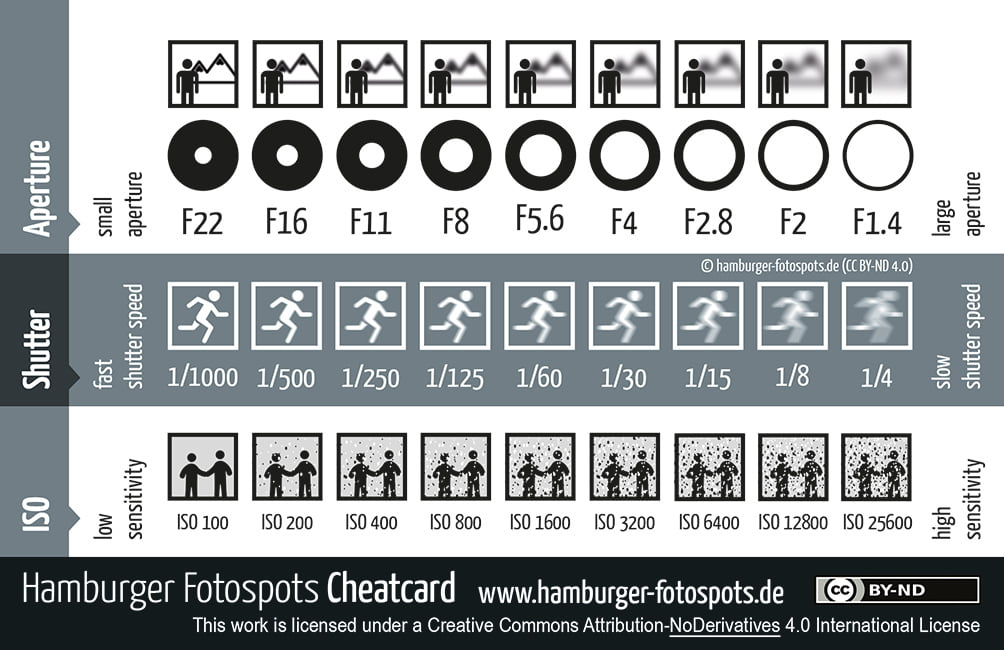
\includegraphics[width=\linewidth]{Fig12_HamburgerFotospots.jpg}
  \caption{Visual explanation of how changing ISO, shutter speed, or aperture changes the resulting photo. Selecting settings towards the right side of the chart will increase the quantity of light collected on the sensor, increasing the brightness of the photo, but will have additional effects that may not be desired. Photo credit: Hamburger Fotospots.}
  \label{fig-cheatcard}
  \end{centering}
\end{figure}

Before discussing equipment in more detail it is helpful to define a bit of the terminology, such as focal length, aperture, shutter speed, and ISO. Figure~\ref{fig-cheatcard} can be used with the explanations to help understand the definitions for the latter three.

\begin{itemize}
    \item {\bf Focal Length}: The distance between a camera lens and the sensor when the subject is in focus, measured in millimetres (mm). It determines how much of the scene the lens captures. Short focal length (like 24~mm) means a wide field of view and captures more of the scene. A long focal length (like 100~mm) means a narrower field of view and zooms in on distant subjects. Standard lenses (approx 50~mm) offer a field of view similar to what the human eye sees, providing a natural perspective. Telephoto lenses (>\,85~mm) have a longer focal length, allowing you to zoom in and capture small, distant details. A wide-angle lens typically has a focal length of 35~mm or less. Common wide-angle lenses range from 14~mm to 35~mm.
    
    \item {\bf Aperture}: The opening in a camera lens that controls how much light enters. Aperture affects both the brightness of your image and how much of it is in focus. It is measured by the f-number (like f/2.8 or f/16). A low f-number (like f/2.8) means a larger aperture, more light, and shallow depth of field (blurred background). A high f-number (like f/16) then means a smaller aperture, less light, greater depth of field (more of the scene in focus).

    \item {\bf Shutter Speed or Exposure Time}: The amount of time the camera's shutter remains open to allow light to hit the sensor. It is measured in seconds or fractions of a second, such as 1/250, 1/60, or 2~s. A fast shutter speed or short exposure (like 1/1000~s) captures a quick moment, freezing motion, and reducing blur. A slow shutter speed or long exposure (like 1/2~s) lets in more light, so is useful in low-light conditions, but can create motion blur if the camera or subject (including an auroral feature) moves.

    \item {\bf ISO (International Standards Organisation):} Measures the sensitivity of a camera's sensor to light. Low ISO (e.g. ISO 100 or 200) is less sensitive to light, ideal for bright conditions, producing clearer images with less noise. High ISO (e.g. ISO 1600 or 3200) is more sensitive to light so is useful in low-light situations, but may result in more noise.

    \item {\bf RAW images:} Unprocessed files from a camera's sensor, preserving maximum detail and allowing for extensive editing flexibility compared to compressed formats like JPEG. 
\end{itemize}

\subsubsection{Lenses}
\index{equipment!lenses}
\index{aberration}
Aurora photography is typically done with wide-angle, large-aperture lenses. A lens with a wide field of view is beneficial for capturing large-scale structures. A large aperture (typically <\,f/2.8) is recommended to increase the light-gathering ability. Wider apertures allow for shorter exposures at fixed ISO, which is important for imaging small-scale or fast-moving auroral features. Standard and telephoto lenses are useful for imaging small-scale auroral features, like fragments (see \ref{fragments}).

Lens quality is a function of sharpness and aberrations. Sharpness is the ability to resolve fine details, while aberrations are any deformation of point-sources of light. The best lenses are sharp across the entire image frame and contain a low level of aberrations. 

The most usual optical aberrations found in lenses are coma, astigmatism, chromatic, and spherical aberrations. Coma aberration causes point-sources to appear with a comet-like tail directed radially towards the centre of the image. Astigmatism gives stars the appearance of ``angel wings'' that are aligned on concentric circles around the centre of the image. Chromatic aberration causes pink and green fringes around point-sources of light. Spherical aberration causes blurring of point-sources of light. Lenses with extra-low-dispersion glass elements work to minimise these aberrations and are becoming more affordable.

Lens material, weight, and other features may affect their ease of use. Lenses with metal construction are heavier but are sometimes more robust against impacts. Plastic or composite-material lenses are lighter and may be more suited for backpacking where weight savings is a priority. Auto-focus lenses can be focused manually but use a ``focus-by-wire'' coupling that can lack a hard stop at the infinity setting. They require careful manual focusing. Fully-manual focus lenses can be easier to set to infinity. But many of these manual lenses do not electronically couple to the camera to transmit their aperture and focal length into the data of the image file. Newer lens models geared towards astrophotographers offer focus lock switches that disable focus adjustments, which is handy for preventing accidentally shifting the focus off infinity. 

\subsubsection{Tripods}\index{equipment!tripods}

%(Contributed - Donna)

A heavy or sturdy tripod is ideal to prevent camera shake during your long exposure. A lightweight one will do for a cell phone, or if you have to hike a long way in to your location. 

It is best to get to know your tripod in daylight. A tripod with a lever for pan or tilt will be easier to adjust in the dark. When selecting, test how easy it is to flip from portrait to landscape mode. You can practise installing the camera, checking focus, changing from portrait to landscape orientation, extending the legs, securing the swivel so that you can do all of these things in the dark. A headlamp will be helpful for some actions that you need both eyes and  hands. When attaching your camera to the tripod in the dark, using a headlamp can help ensure a secure mount and prevent accidental falls. After securing the camera, test the connection by gently wiggling it while still holding on. This way, if the mount is loose, you'll have a firm grip on the camera, reducing the risk of it falling.

If you want to take low-angle shots from the ground, your tripod might not be able to go low enough. In such cases, you can improvise by using something to support the camera, keeping it off the wet or muddy ground. This way, you can still capture those unique low shots without damaging your gear.

\subsubsection{SD Cards}
%\contributed{Donna}
Not all SD cards are equally as effective.   Here are a few things to note when purchasing your SD card:
\begin{itemize}
    \item \textbf{SD > SDHC > SDXC}: This is the evolution of the SD card type, which indicates the file system used. The most recent will allow more storage space.
    \item \textbf{Capacity:} Indicates the storage on the card, for example 128~GB.
    \item \textbf{W = Write Speed}: Indicates how fast the data can be written onto your card, which can translate to how fast your photo can be taken.
    \item \textbf{R = Read Speed}: Indicates how fast your data can be read off the card for transferring to your computer.
    \item \textbf{Speed Class}: C10, U1, V10 will all write at 10~MB/s. If you take video and would like to produce 4K, you will need V60 or higher.  
    \item \textbf{Video: } Use V cards and check the video resolution capabilities if you want high quality. 
    \item \textbf{CFexpress:}  If you are taking video and considering this type of card, check if your camera is compatible.
    \item \textbf{I or II Bus Interface:}  Indicates how fast the data can be transferred off the card.  II is the fastest.  Older cards have become obsolete and will be very slow if you try to use them.
    \item If you wish to reuse your SD card after removing the photos, it is recommended that you wipe the card and format it.
\end{itemize}

\subsubsection{Timelapse Equipment}\index{photography!timelapse}

%(Contributed - Donna )
\begin{itemize}
    \item\textbf{Intervalometer on Camera:} Internal or external.  Photos can be imported to your computer and processed in a program like Lightroom, or other software (e.g. RawTherapee, Darktable), and then compiling the images into a video with a frame rate of your choice.

    \item\textbf{Camera Phone:}  The timelapse setting can compile the timelapse in the application itself.

    \item\textbf{GoPro:} Night lapse setting can compile the timelapse in the application, or photos can be imported to your computer for processing.

\end{itemize}


\subsection{Camera Settings}\index{photography!camera settings}
\subsubsection{Single Shot}\label{single-shot}
Since your camera will be capturing long exposures, it is important to keep it stable to avoid any movement. A tripod is essential for this! To further reduce movement when taking a shot, consider using a remote shutter release or setting your camera to have a 2-second delay after pressing the shutter button.

For cameras with manual settings, such as DSLRs or mirrorless models, set the ISO between 1600 and 6400, with 3200 being a good starting point. Adjust the aperture to its lowest setting or keep the lens wide open; ideally, this should be lower than f/2.8, although some lenses may only go down to f/3.5. Begin with an exposure time of 5 to 10~s. You will need to adjust ISO and shutter speed to achieve optimal results, which will vary based on what you are photographing, the available light, and your desired image outcome. This process involves some experimentation. If the photo appears too dark, increase the ISO or extend the exposure time. Conversely, if it is too bright, decrease the ISO or shorten the exposure. Keep in mind that these recommended settings may yield different results depending on your specific camera.

Many modern cameras are so called ISO invariant\footnote{See a list of camera models which can do this in 2024: \url{https://capturetheatlas.com/iso-invariance/\#models} and more for thorough explanation: \url{https://theauroraguy.com/blogs/blog/iso-is-not-what-you-think-it-is-what-is-iso-really\#:~:text=ISO-invariant\%20cameras\%20have\%20lower,the\%20exposure\%20in\%20post-production}}. That means that RAW images can be taken at low ISO, for instance ISO 400 instead of ISO 1600, which basically underexposes the image. The exposure can be increased in the post-processing (in software like Lightroom or RawTherapee) to correspond to higher ISO without overexposing the brightest features in the image. However, the image quality in terms of noise, colour and other properties remain the same. This new way of capturing photos with great dynamic range is possible because the image readout noise is minimal.

For smartphones, success will depend heavily on the age of your phone, with newer models being more effective than older ones. If your phone has a night mode, be sure to use that feature. If your phone offers manual settings, apply the recommended values mentioned earlier. For older iPhones, consider using the NightCap camera app. Newer Google Pixel phones also have an astrophotography mode that can be particularly useful.

\subsubsection{Timelapse Imaging}\index{photography!timelapse}\index{photography!single shot}

Some good practices for timelapses are listed below: 
\begin{itemize}
    \item Short intervals will make a smoother timelapse. Continuous shutter, or 1-second interval will show the evolution of the formations better. However, this will use a lot of space on your SD card.
    \item If the aurora is bright enough, a short exposure of a few seconds (or as short as 1~s) will help show fine-scale structures.
    \item Take the time to set up your camera in a good position, and leave it there for the entire observation. If you must move its position, it is better to have 400~photos in one position than 50~each of 8~different positions.
    \item If you are in the subauroral region wanting to capture subauroral features, it is a good idea to aim eastwards or westwards along the oval. This perspective enables you to see features that are equatorwards of the main aurora.
    
\end{itemize}

\subsubsection{Photographing Aurora with Other Phenomena}

\begin{figure}[h!]
\begin{centering}
  \includegraphics[width=\linewidth]{Fig13_HaloCloud.png}
  \caption{Photos combining aurora with Moon halo (top) and noctilucent clouds (bottom). Photo credit: Eero Karvinen.}
  \label{fig-aurorahalonlc}
  \end{centering}
\end{figure}

You might want to capture other atmospheric phenomena alongside auroral displays. By selecting the right season, you can increase your chances of photographing the desired effects. For example, the Moon can create Moon halos that shine brightly, sometimes outshining the aurora, as seen in the top photo of Figure~\ref{fig-aurorahalonlc}. Combining these two elements can yield breathtaking images.

In summer from mid-latitudes, noctilucent clouds can be observed alongside the aurora, resulting in beautiful wavy photographs featuring blue and white hues, as shown in the bottom photo of Figure~\ref{fig-aurorahalonlc}.

Occasionally, distant lightning can coincide with the aurora, providing a chance to glimpse sprites above distant thunderclouds. Comets may also be visible with the aurora. Additionally, airglow can sometimes be bright enough to add extra green and red colours to your aurora photos. You might also consider incorporating human-made elements into your images, such as planes, rocket launches, fireworks, campfires, car lights, or city lights, which can create attractive effects.




\subsection{Image Processing}
%\contributed{Les Ladbrook and Katie }

\begin{figure}
  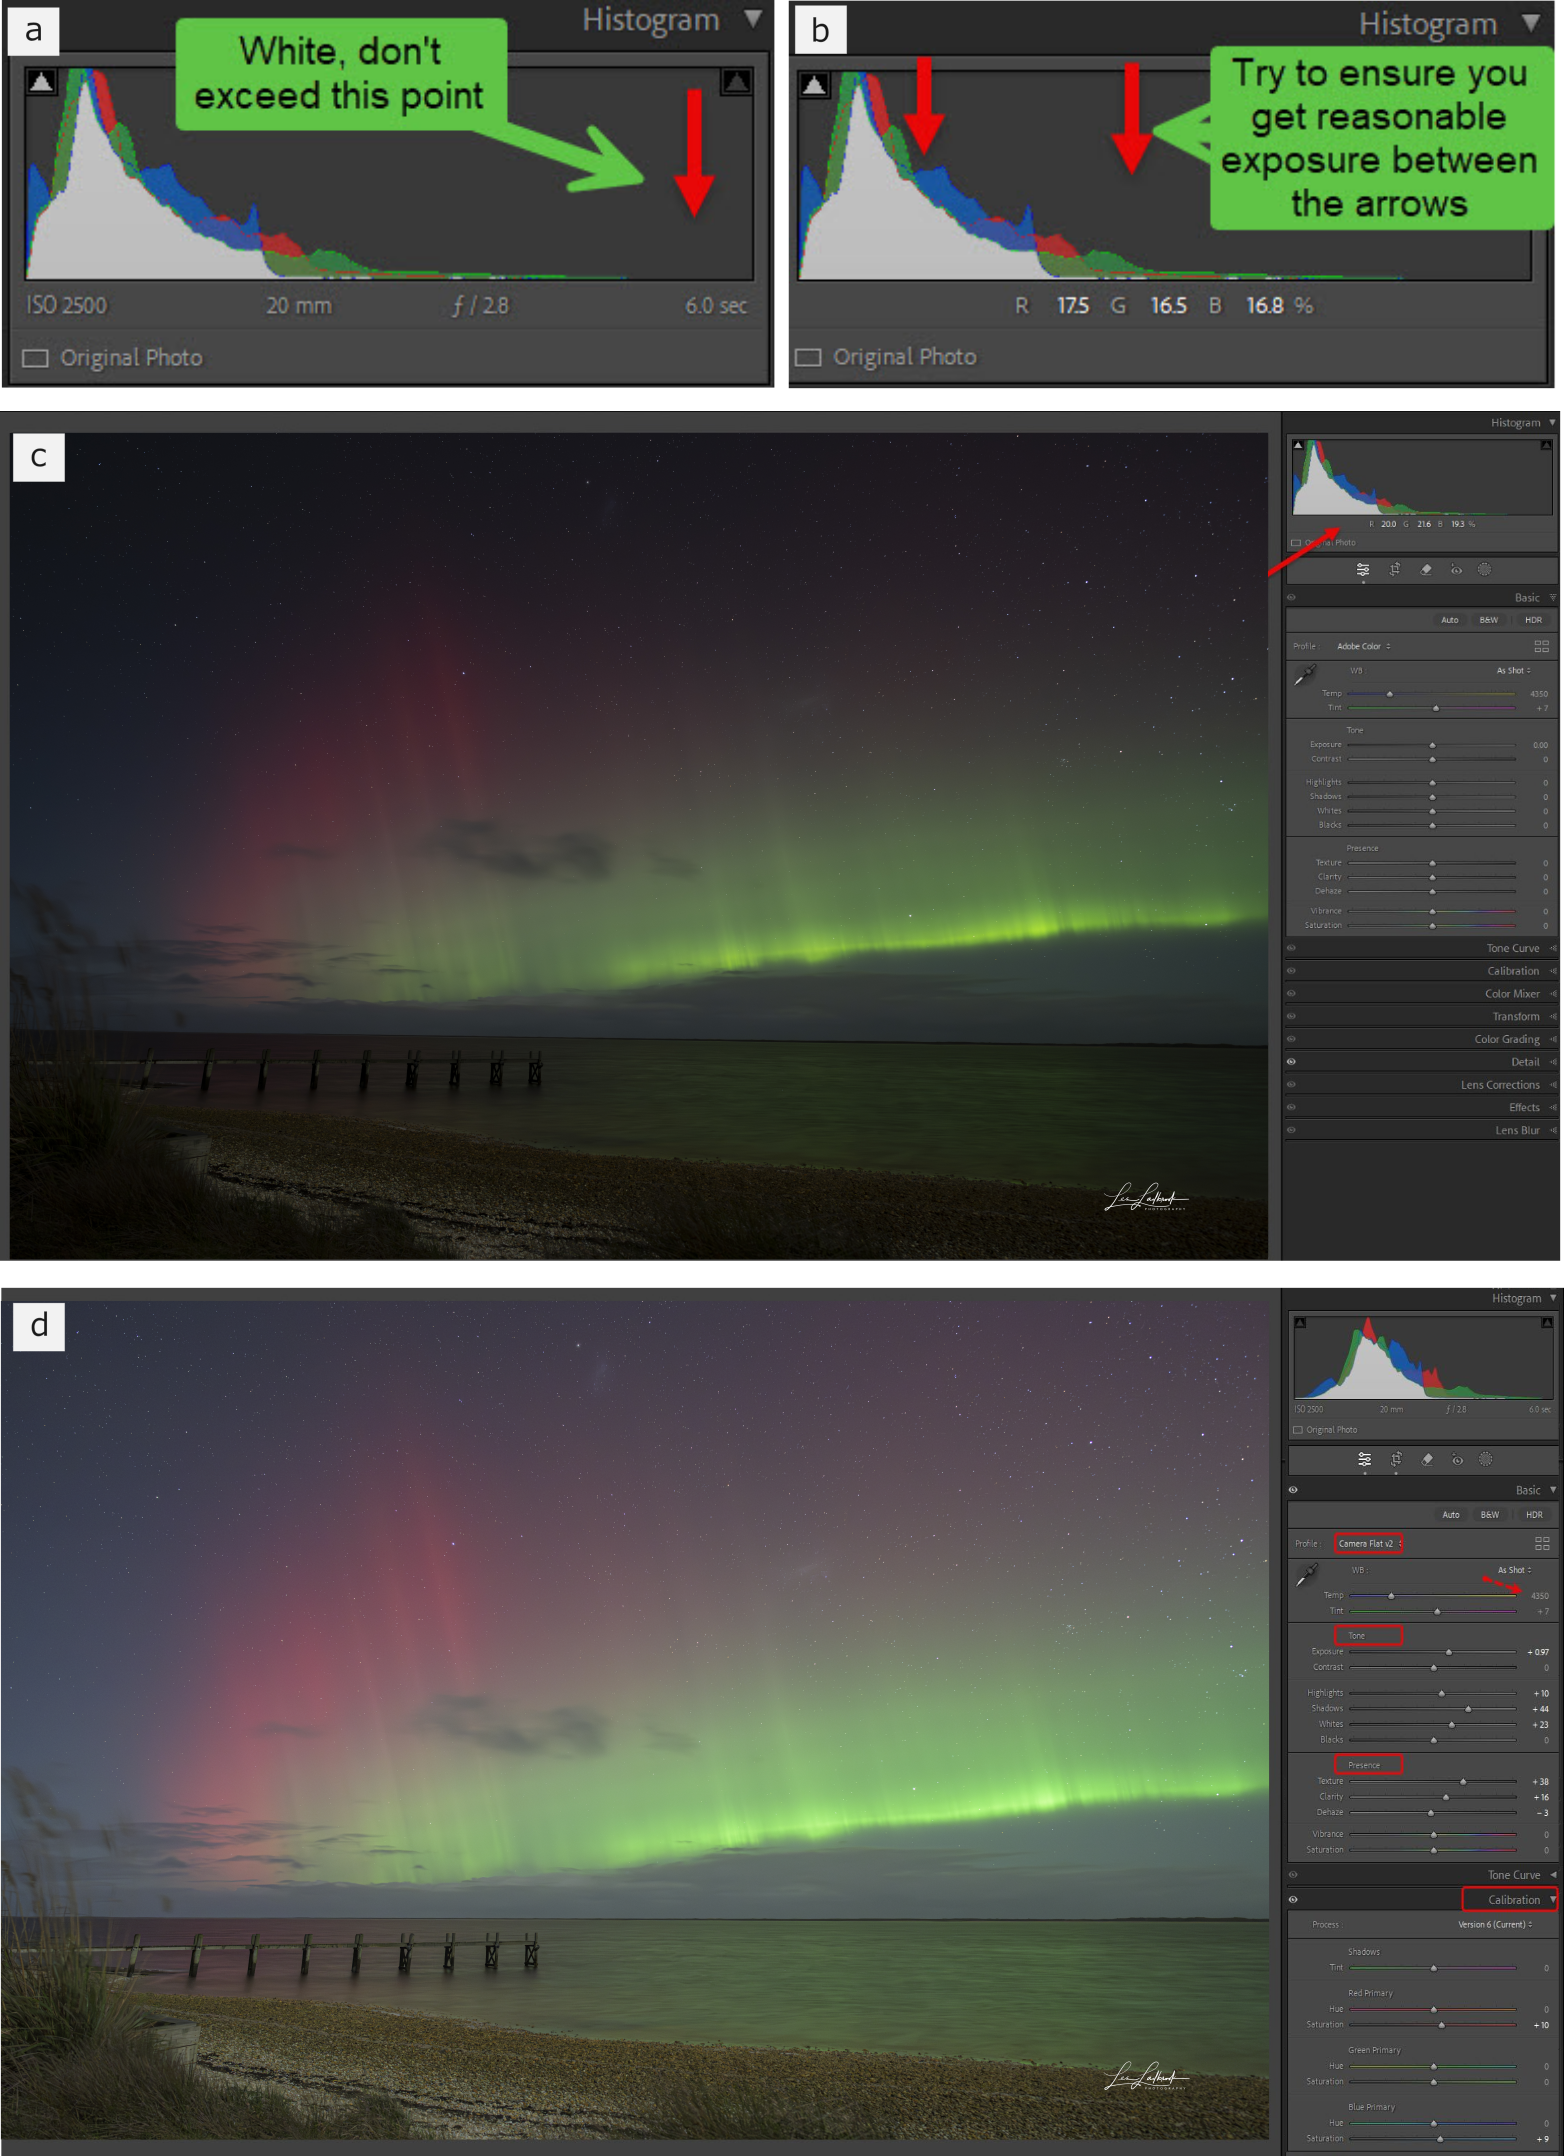
\includegraphics[width=\linewidth]{Fig14_ImageHistograms.png}
  \caption{An example of how to process an aurora image. Panels a) and b) advise on the shape and extent of the histogram, c) shows the image as shot, and d) shows the processed image. Credit: Les Ladbrook.}
  \label{fig-processing}
\end{figure}

The first step in creating an auroral image is to shoot RAW images, which saves more image details and gives more possibilities to edit the image in the processing phase. Next, ensure that your captured image has a good exposure without blown-out highlights. The image in Figure~\ref{fig-processing} was taken with a 20~mm lens at 6.0~s exposure, f/2.8, ISO 2500, under approximately 48\% moonlight. The exposure settings will vary depending on the brightness of the scene. If you shoot with a Camera Flat or Neutral profile (in camera), during processing in Lightroom (or equivalent software\footnote{If you do not wish or cannot afford to purchase a Lightroom licence, you may want to consider using free alternatives such as RawTherapee or Darktable.}) you can choose the same profile within the software.  Shooting with your camera set to ``Camera Flat'' gives you the widest dynamic capture range of the camera, so this is a recommended setting. 

After capturing the image, check your camera's histogram to confirm that highlights are not blown out and that the exposure is correct -- underexposure can lead to excessive noise. Make sure no part of the histogram extends beyond the red arrow in Figure~\ref{fig-processing}a. Aim to achieve good detail within the range between the two arrows in Figure~\ref{fig-processing}b. Figure~\ref{fig-processing}c displays the original image with the histogram indicated with a red arrow, while Figure~\ref{fig-processing}d shows the image after processing in Adobe Lightroom. Notice the histogram shift, indicating the image has been brightened (appears brighter on a backlit screen). To adjust the histogram, tweak the sliders for exposure, highlights, shadows, whites, texture, clarity, and dehaze. Use dehaze sparingly and avoid saturation. Use the calibration tab (indicated in Figure~\ref{fig-processing}d) to enhance colours instead of using vibrance or saturation in the presence section, which adjusts colours in a very subtle way. Apply a small amount of sharpening, with a mask to focus primarily on the foreground, avoiding the sky, and use noise reduction as needed. For example, Lightroom’s enhance option can be used to sharpen the image. The final look of a processed image is subjective, so feel free to experiment to see what you like! For communicating with scientists, it is preferable if the feature of interest can clearly be seen in the processed image. 



\subsection{Tips \& Tricks}


\begin{figure}
  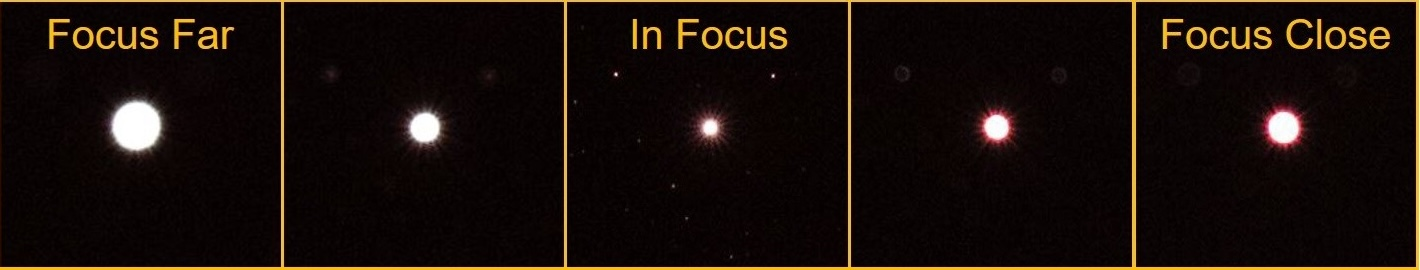
\includegraphics[width=\linewidth]{Fig15_focusing.jpg}
  \caption{Sequence showing how when a point light source is in perfect focus, it appears smallest and sharpest. On either side of this focus point, the light grows larger and blurrier.}
  \label{fig-Focusing}
\end{figure}



Below are some tips and tricks for when you are out in the field taking your aurora photo:

\begin{itemize}
    \item Buy some extra camera batteries and take them with you! Keep them close to your body to keep them warm so that they last longer.
    \item Get the precise time and location of your photos so they can be used for science. If your camera lacks GPS, use your phone's GPS and take a photo of your camera's time. This will provide you with both the exact time and location, allowing you to adjust for any discrepancies in your camera's time later. Also taking a camera photo of the \url{www.time.is} site and saving that with the photos from each observation session is helpful.
    \item Use a red headlight to preserve your night vision and change the colour scheme to dark mode on your phone or camera.
    \item Use the two-second self timer, so that when you press the button on the camera to take the photo, the camera shakes and settles down before the exposure begins. This means there is less risk of your photo blurring.
    \item If you do not focus your camera correctly, you might not notice on the small camera screen, but then see that everything is blurry when loading the image on the computer. Slow down, take a second, and focus properly! 
    \item When taking aurora photos, aim to focus at infinity, though the precise focus point might be slightly back from infinity. To fine-tune your focus, zoom in on a distant point of light, such as a streetlight or a light on a mast. Use your camera’s live view to digitally zoom in as much as possible. If the light appears as a donut shape, adjust the focus until it becomes a sharp point. See Figure~\ref{fig-Focusing} for an example of what this looks like. After taking a few shots, zoom in on a star in the photo to ensure it’s in sharp focus. Periodically recheck the focus to ensure it has not been accidentally shifted.
    \item When focusing on smartphones, tap to focus on the sky so that no objects in the foreground are targeted. You can also use a manual focus on some phones to focus to infinity on the stars. Check your images to see that the stars are sharp when you zoom in on them.
    \item If your camera did not acclimate to the air temperature and your lens is accumulating condensation or frost, wipe it often with a microfiber cloth. This is important, since you will not manage to salvage foggy or frosty photos by post-processing. For long timelapses, using a lens warmer or anti-dew heater band can ward off frost in winter and dew in summer. 
    
\end{itemize}



\section{Imaging for Science}\label{imaging-for-science}\index{contributing!imaging} 


This section covers metadata recommendations, camera and scene settings for different types of aurora, different types of citizen scientist imaging platforms, and advanced equipment.

\subsection{Metadata Recommendations}\index{data!metadata} 

As a first step, when a citizen scientist takes a picture of the aurora, the timestamp and latitude, longitude, altitude coordinates are mandatory for any scientific interpretation. To be most useful, the precision should be better than 1~min for the timestamp and better than 100~m for the coordinates. A precision of 1~s and less than 10~m is really great.
These parameters allow scientists to localise the aurora and if several pictures of the same auroral structure are taken at the same time, it could allow triangulation and then a determination of the altitude of the different features. This is interesting because the altitude correlates with the energy of the incoming electrons.

To allow determination of the intensity, it is then better to add in the metadata, the kind of camera, the exposure time, the kind of lenses and the aperture.

For most cameras these metadata are included in the file but this is not the case for every camera. For those that do not record the metadata, include the information in the comments or captions. 

In summary, the following information is needed for general scientific use:
\begin{itemize}
    \item \textbf{Location:} GPS coordinates (10~m accuracy)
    \item \textbf{Date \& Time:} Recorded in Universal Time (1~s accuracy)
    \item \textbf{Camera Settings:} Exposure time, aperture, ISO
    \item \textbf{Setup Description:} Type of camera and lens
    \item \textbf{Raw Data File:} Provides the most information if available
\end{itemize}

\subsection{Observation Time}\label{data_cit_time}\index{data!metadata}

All observers are able to improve the quality of their collected data by simple means. Applying these requires instructions, communication and routine. Communicating these needs and making them a repeated part of event recording routine as early as possible saves time later in the observation analysis phase.

When making observations of northern or southern lights, the most important detail to remember is to ensure that the camera's clock is accurately set before shooting a display. If the observer forgets to check the time, it can be done immediately afterwards by comparing the time shown by the observer's mobile device to the time still shown by your camera. Taking a photo with your smartphone of the camera's clock and saving it in the image folder with the associated material is considered good practice. 

Having access to the exact time of the image guarantees that the image can later be connected to additional data sets like satellite or ground-based observations. Measurements from different scientific instruments can often explain the recorded phenomenon, if citizen scientists' observations can be connected to it by exact timing information. If the exact observation times are missing from the image material, it becomes largely useless for scientific purposes. 

\subsection{Camera Settings for Science}\index{photography!camera settings}
Earlier we provided tips for capturing the aurora and basic aurora photograph processing. However, the best images for science are not necessarily the most beautiful ones. Camera processing software can degrade the pictures in an unknown way compared to the raw data. We will now discuss some important aspects and advice for choosing camera settings for photos that can be used most effectively for scientific research.

\subsubsection{White Balance}
It is crucial to maintain a consistent colour balance, as the ratio between the green, blue, and red channels contains valuable information. To achieve this, shoot in raw format with a fixed white balance of 5200~K, equivalent to daylight colour temperature. Avoid using Auto White Balance, as it can result in varying colour balance from frame to frame.

\subsubsection{Bit Depth and File Format}
Always shoot in RAW format, not JPG. RAW files allow for adjustments to correct and standardise the white balance later. Additionally, RAW files have greater bit depth. Depending on your camera, each pixel is encoded with a specific number; for instance, in a 12-bit file, pixel values range from 0 to 4095. Converting from RAW to JPG scales these numbers down to a range of 0 to 255, reducing the precision of intensity and the image quality. This loss can hinder our ability to accurately reconstruct the intensity for each pixel.

\subsubsection{Exposure Time}
For scientifically useful images, consider the type of photos to take. Capturing fine-scale structures may require a longer focal length, while large-scale changes necessitate a wide lens to cover more of the sky. In both cases, use the widest possible aperture and a reasonably high ISO value, typically between 1600 and 6400. While higher ISO settings can introduce more noise, they allow for shorter exposure times, reducing motion blur from the aurora's movement. Aim for exposure times shorter than 1/2~s, which usually requires lenses with maximum apertures of f/1.8 or f/1.4.

\subsubsection{Imaging Location}
Choosing the right location is also important. Avoid light sources, since light pollution and even moonlight can wash out faint aurora, such as SAR arcs (see \ref{steve-sar-arcs}). For scientific observations, it is best to have minimal or no moonlight. Open areas are ideal, and many photographers prefer seascapes or lakes to reflect the aurora. Ensure the horizon line is horizontal and position trees and other objects as desired in your composition.

\subsubsection{Short-Lived Transient Features}\label{short-lived-transient-features}
To capture features that only exist for a short period of time, or that evolve quickly, the camera exposure time will need to be shorter than 1~s. To achieve this, the ISO might need to be increased to the point where a lot of noise becomes apparent in the photo, unless an ISO invariant camera is used (see \ref{single-shot}). Some examples of this kind of feature are fragments (see \ref{fragments}), or rapid dynamics during a substorm breakup.
\index{fragments!camera Settings}


\subsubsection{Fine-Scale Structures}

The aurora can include a lot of different fine-scale structures. These are often transient phenomena like pulsating aurora or thin fast-moving rays and flows. Some auroral phenomena have such a rapid motion that ordinary cameras are not fast enough, but many kinds of fine structures can be photographed by ordinary digital cameras. Special attention is needed for photographing these fine-scale details. Be ready to switch your camera into the settings that might be better suited to capturing fine-scale features, such as switching to a higher ISO, rapid burst modes, or even a movie mode. Or switching lenses to a longer focal length. Remember that this opportunity may arise suddenly. The most important thing is to keep the exposure time as short as possible because of the dynamic movement of aurora. One second or less is the preferred exposure time. Many new camera models automatically set the ISO value if the exposure time is manually set. Suggested ISO values could be 3600 to 25,600. Some new cameras have huge ISO values like 100,000 and these values can be tried but the noise could be an issue. Fast apertures are usually needed. By using these extreme ISO values combined with large-aperture lenses, some camera models are able to take several to tens of high-resolution images per second. Using a large aperture and high ISO values with the maximum aperture of f/1.2 to f/2.4 is therefore preferred. 

The focal length can be chosen to be suitable for the size of the phenomenon. 50~mm or 85~mm are good focal lengths for recording photos of small-scale events like STEVE and picket fence (see \ref{steve-sar-arcs}) or fragments (see \ref{fragments}). For the larger-scale events like the dunes (see \ref{dunes}) and auroral coronae, 14~mm or fish-eye lenses are a better choice. Timelapse imaging is sometimes important for seeing the movement of the fine-scale structures.


\subsubsection{Real-Time Movies}
Rather than taking still images, consider shooting a movie of fast-changing auroral phenomena. Low-megapixel (12 to 24 Mp) mirrorless cameras can take good low-light 4K movies that can record the motion of fine-scale structures better than timelapses or a burst of images. Cameras good for this include the Sony a7s series, Canon's R6 and R6MkII and Nikon's Z6 series. When shooting at 24 or 30 frames per second, the shutter can be set to as slow as 1/8-second (Canon) or 1/4-second (Nikons/Sony), called a ``dragged'' shutter speed. This is still fast enough to record motion without too much blurring of detail and allows the ISO to be kept lower for less noise, though the ISO might still need to be 12,800 to 25,600. 

While movies can be shot in RAW formats, the files can massive and hard to process. Inevitably, they will need to be converted to a compressed H.265 or H.264 format for distribution. Shooting in a compressed format to begin with in the camera should still work well for science purposes.

\subsubsection{Dim Aurora and Large-scale Structures}\label{DimAurora}
\index{proton aurora!camera settings}
\index{dunes!camera settings}


Proton auroras are a part of the main oval. They appear as diffuse structures and are discussed in \ref{proton-aurora}. More interesting proton auroras are sometimes present equatorwards of the main oval. There is usually a clear gap between these isolated proton auroras (IPA) and the main auroral oval. IPA usually appear faint and diffuse. Many citizen scientists have identified the colour as a blueish tint. 

The shape of these proton auroras is mainly blobs that appear and disappear slowly in periodic pulses. Sometimes arc or sausage-like shapes can also be seen. Proton aurora relates to the substorm evolution, and therefore the best time to observe it is on the nightside of the planet at the location where plasma convection flow changes from westwards to eastwards (named the ``Harang reversal'' region in scientific literature).

In some cases, we can see faint red arcs or rayed structures over these greenish blobs. The phenomenon is named ``RAGDA'' (see \ref{proton-aurora}), discovered by citizen scientists \cite{Nishimura2022}. 

Photographing an isolated proton aurora and RAGDA is not easy because of the faint appearance. Both are photographed at the same settings. The best way is to use a high ISO value, perhaps ISO 1600 to 3200 and the largest aperture possible. An aperture of f/1.4 to f/2.4 is preferred. As these features are usually faint and slow moving, exposure times of 10 to 30~s are usually needed for good photos. It may be a good idea not to aim the camera at the main oval directly because it will be overexposed/visually dominant. The location plays an important role. A geomagnetic latitude of 55\textdegree to 65\textdegree is preferred as IPAs are a subauroral phenomenon. Also, if the photographer is situated in the gap between the IPA and the main oval, it makes the photography easier because isolated proton aurora blobs can be photographed separately.

Dunes (see \ref{dunes}) have a lot of similarities with proton aurora. Dunes can be seen at the diffuse part of the auroral oval (the ``dune shelf'') during the substorm growth phase in the evening sector. Dunes are best photographed by taking the photo westwards or eastwards along the oval. Usually long exposure, 10 to 20~s with 1600 or 3200 ISO is needed and the largest aperture is recommended.


\subsection{Organising Aurora Photos}\label{data_cit_storage}\index{data!storage}

When organising aurora photos, a good method is to split the material into event folders. The folder name should contain the year, month and day of the event. Since the day might not uniquely identify the night ISO 8601-inspired naming like 2024-03-23-24 could be used. The last two pairs of numbers indicate that the event happened between the night of 23th and 24th of March, 2024. Storing the observation location to the end of the folder name helps the observer ensure that the second most important piece of metadata is attached to the set of images (for example 2024-03-23-24\_Auroras\_Calgary).

When the collected photos are organised in a structured fashion, the next step is to secure that backups of the collected image material exist. The most secure way is to copy/mirror your material to a storage space outside your home or other primary storage location. At minimum, a separate USB-drive could be used to secure a local duplicate of the observation image data.

For saving disk space, it is often tempting to reduce the amount of saved images. However, many of the discovered new phenomena can be faint or a small-scale feature in the aurora display. This means that if the only the brightest moments of an aurora event are saved, much of the fainter -- and potentially valuable -- material is lost. Hence it should be emphasised that visually unimpressive image material and aurora features can also have scientific value, even if it does not look as spectacular.



\subsection{Citizen Scientist Imaging Platforms \& Equipment}
There are some purpose-built imaging platforms or other advanced equipment that citizen scientists either develop themselves or can be sent to collect and analyse data. These are primarily all-sky cameras, and notable projects include the AurorEye and NoDDAC projects.

\subsubsection{AurorEye}

Led by Jeremy Kuzub, the \href{https://auroreye.ca/}{AurorEye project}\footnote{https://auroreye.ca/} is leading the development and deployment of portable all-sky imagers for aurora chasers to install in the field and take timelapse images \cite{Kuzub2022}. Aurora chasers are provided with a large-sensor RGB all-sky imager packaged as a self-contained, highly portable ruggedised unit with minimal setup and operation steps. Examples of AurorEye units deployed in the field can be seen in Figure~\ref{fig-auroraeye}. This unit can be brought on nightly aurora chases and operate for a full night in cold conditions without external support. AurorEye is designed to autonomously capture timelapse imagery and upload it to a central location via wireless communication on return from the field, including GPS location and other metadata. Hardware is primarily consumer-off-the-shelf (COTS) components controlled by a low-cost Raspberry Pi single board computer. The system is flexible enough to incorporate a variety of makes and models of cameras and lenses while providing sufficient room for additional future instrumentation, such as magnetometers. The resulting data can be integrated into other citizen science projects such as Aurorasaurus (see \ref{aurorasaurus}) or Skywarden (see \ref{skywarden}) and pre-processed data products (e.g. keograms) are automatically generated after each image sequence. The AurorEye project is just one way citizen science observations can be compared with science-grade instrumentation data, when it is time and location synchronised, and operated by enthusiastic local experts who know their skies. It demonstrates the value of synchronised observations in order to become part of the larger instrumentation network. 

\begin{figure}
  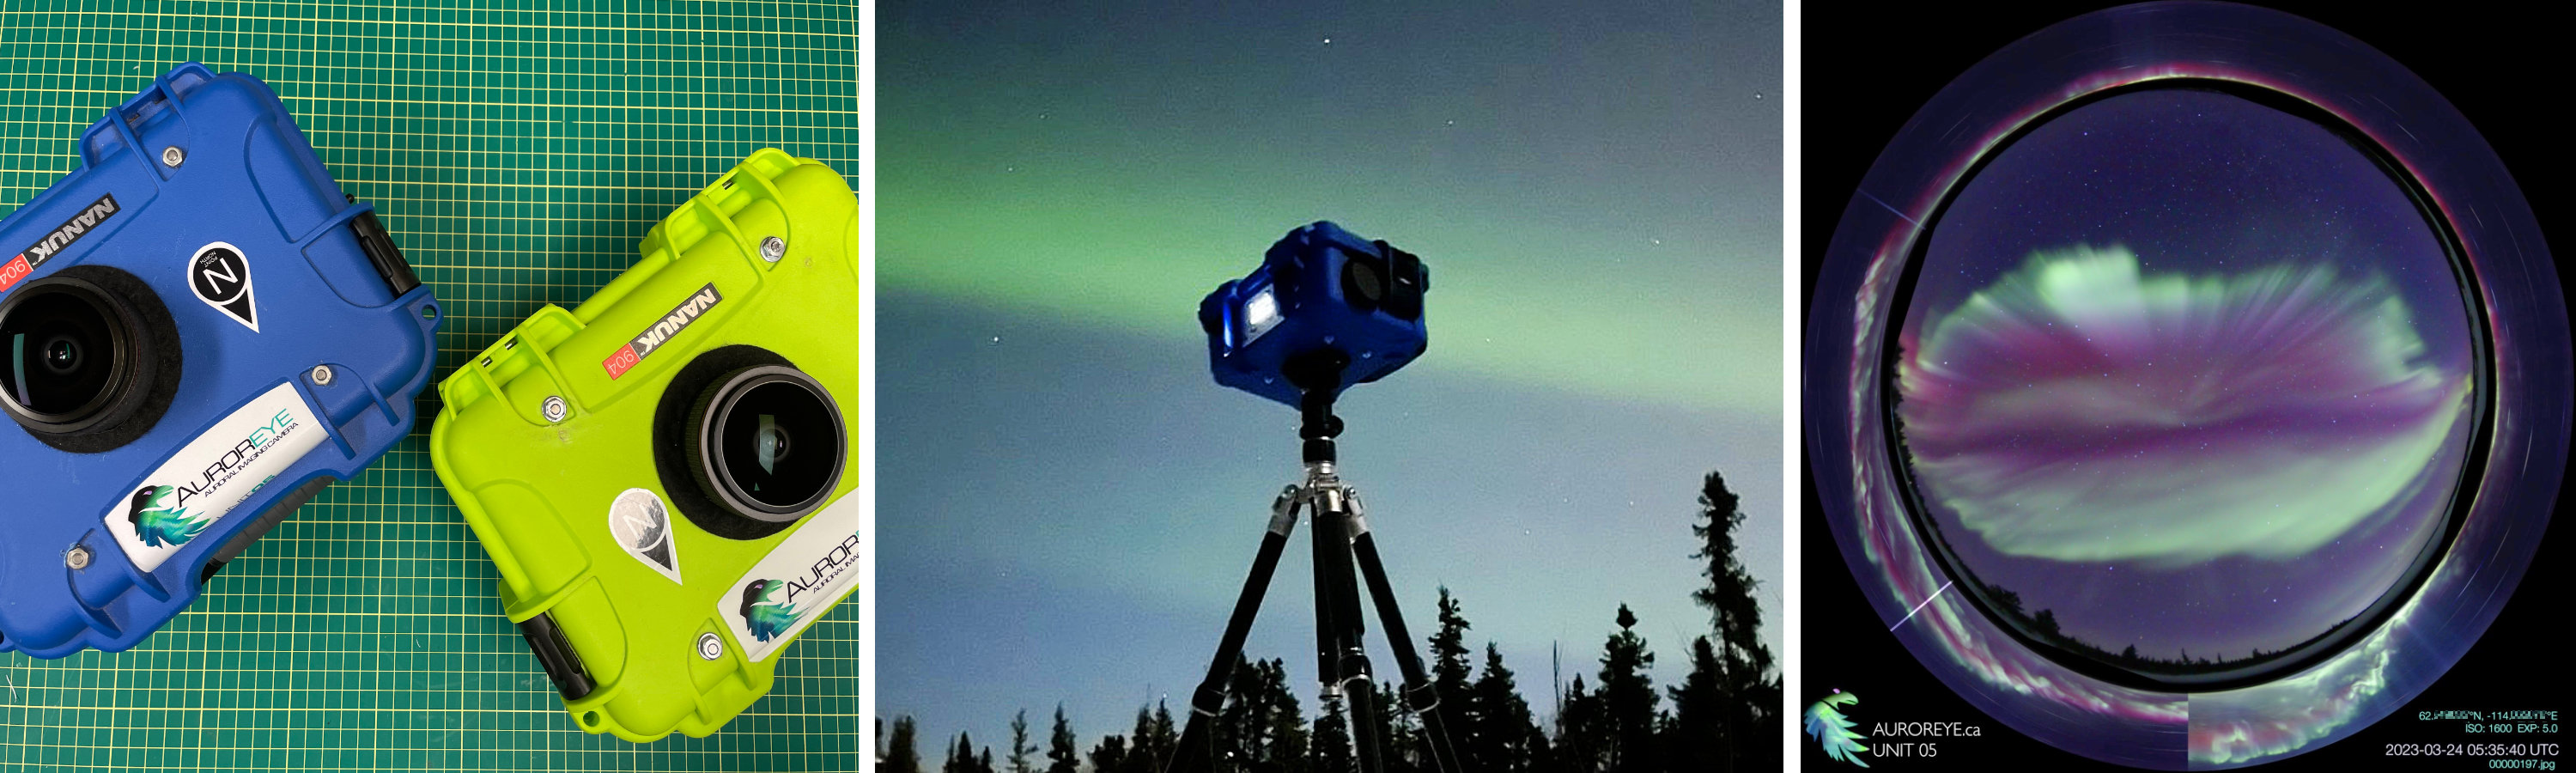
\includegraphics[width=\linewidth]{Fig16_AurorEye.jpg}
  \caption{Left to right: AurorEye Units 4 and 5; Unit 5 deployed in Fairbanks, Alaska; All-sky image with a keogram ring. Photos captured by Jeremy Kuzub and Vincent Ledvina.}
  \label{fig-auroraeye}
\end{figure}

\subsubsection{North Dakota Dual Aurora Cameras (NoDDAC)}

Founded in partnership with the University of North Dakota (UND), Aurorasaurus, and the Live Aurora Network in 2021, NoDDAC (North Dakota Dual Aurora Cameras) provides permanent observations of the mid-latitude aurora from North Dakota through the use of a north-facing video camera and an all-sky stills camera (hence the name ``dual''). There are now two NoDDAC locations: the UND Physics \& Astrophysics Department's Martens Observatory (48.1\textdegree N, 97.6\textdegree W) and the Nueta Hidatsa Sahnish Tribal College (NHSC) located 480~km due west of Martens Observatory. Together, these two locations provide stereo views of the aurora and help capture rare mid-latitude auroral (or aurora-like) phenomena, such as STEVEs, SAR arcs, and dunes. Both cameras and installations use COTS equipment and software. Popular Sony camera models record images and video of the aurora, and file handling and image uploading is managed by IPTimelapse software. The north-facing video camera from Martens Observatory is live streamed on the NoDDAC \href{https://www.youtube.com/@northdakotadualauroracamer7115}{YouTube channel}\footnote{https://www.youtube.com/@northdakotadualauroracamer7115}. Images from the all-sky cameras are archived on a public-facing aurora database. Aurora sighted by NoDDAC will soon be incorporated into Aurorasaurus to provide alerts to nearby chasers. A Zooniverse citizen science is currently in the works to help classify and analyse the thousands of aurora images NoDDAC has captured since 2021.

The approximate cost of both AurorEye and NoDDAC are between \$5000 and \$10,000~USD. Because both projects use COTS equipment, it is feasible that an enthusiast chaser would be able to collaborate with these projects to obtain their own units.

Low-cost solutions to science-quality auroral imagery are already being employed in other projects. For example, the University of Alaska's Space Weather Underground (\href{https://sites.google.com/alaska.edu/swug/home}{UAF SWUG}\footnote{https://sites.google.com/alaska.edu/swug/home}; \cite{cohen2024}) program has implemented a low-cost \href{https://prinsfrank.nl/2024/02/13/Building-an-all-sky-camera}{all-sky camera}\footnote{https://prinsfrank.nl/2024/02/13/Building-an-all-sky-camera} developed by Frank Prins, an industry software engineer, with plans for many units to be deployed to high schools across rural Alaska. Along with NoDDAC and AurorEye, UAF SWUG's effort highlights the opportunities for private-public partnerships and the relative ease at which COTS technology can be used for real scientific purposes.

\subsubsection{Spectrometers}
A large set of spectrometers exists for amateur photographers or astronomers. They come with various characteristics which can be convenient for auroral observations. We chose here to give an overview of the main technical characteristics of the spectrometers that can help amateurs to use these instruments on the auroral observations.

Spectrometers are generally devices that use a grating (or for old spectrometers a prism) to disperse the different wavelengths (colours) of the light. The light enters the instrument via a narrow slit and is projected onto a camera after dispersion. This means that for regular spectrometers only one small area of the sky can be seen. 
Spectrometers are characterised by their focal length, the width of the slit, and the dispersive power of the grating, generally in number of lines per mm. A typical grating has 300~lines/mm. A very dispersive grating can reach 2400~lines/mm. Since the light is dispersed by the grating, and the slit is narrow, the sensitivity of spectrometers is low and requires a long exposure time to enhance the signal over the noise.

The spectra of the aurora carry information on the relative or absolute intensity of the different emission lines (or colours), which in return can be used to estimate the altitude of the emissions and the mean energies of the precipitating particles. Recent measurements made with different spectrometers have revealed characteristics of continuum emission (see \ref{continuum}) in the aurora \cite{Gillies2019}, which in photos look just grey/white.



\section{Identify \& Report Auroral Phenomena}\index{contributing!as a citizen scientist}
This section outlines how to identify different types of aurora and how to report your observations to an online observation system.

\subsection{How to Identify Phenomena}\index{identification!how to} \

This Handbook contains brief descriptions of different phenomena to help with the identification in \ref{types-of-aurora-and-optical-emissions}, which also contains links to examples and descriptions on Skywarden (see \ref{skywarden}). We at ARCTICS have also created a \href{https://kherli.github.io/Aurora-Field-Guide-And-Handbook/_static/Aurora_Field_Guide.pdf}{Field Guide} with example photographs of many different types of aurora and optical emissions. We suggest that you download and use it as the easiest way to identify features out in the field and afterwards.

Keep in mind that it is absolutely fine to submit aurora photos to online databases without classifying them yourself! Classification can be a complicated matter. If you are curious about what you see but unsure how to classify your image, others, such as the Skywarden moderators, can help with the process by reviewing your observation after submission. The threshold for submitting to an aurora database should be low, so do not worry about needing to classify the images or making mistakes in your attempt. However, if you are eager to start learning how to classify the aurora you capture, here are some tips and helpful questions to ask yourself:
\begin{itemize}
    \item \textbf{Colour and Shape:} Is the aurora red/green/blue/white? Something else? A mixture? Is it a long thin arc, small repeating chain of aurora, longer fingers of repeating aurora, a diffuse/fuzzy blob? Does the aurora show a spiral-like shape? Is the aurora aligned in a specific direction?
    \item \textbf{Brightness:} Would you be able to see it with your eye? Is this as bright as any surrounding aurora?
    \item \textbf{Location:} Are you taking photos of the poleward edge of the auroral oval, the inside of the oval, or the region equatorwards of the oval? You can also think about the time of day that you are making your observation or whether it was before, during, or after a substorm (see \ref{auroral-substorms}).
    \item \textbf{Duration and Stability:} Does the aurora disappear after a few seconds, minutes, or hours? Does it move in a certain direction, either slowly or quickly? Does it keep the same shapes and colours or transition from one to another?
    \item \textbf{Your Camera Settings:} Keep in mind that your camera settings can change the shape or colour of the aurora. So it is worth considering how your exposure time or white balance could affect your photo (see \ref{imaging-for-science}).
\end{itemize}


\subsection{Types of Aurora and Optical Emissions}
\label{types-of-aurora-and-optical-emissions}
%\contributed{Donna, Emma, Noora}

The aurora can appear in many shapes, colours and types of movement.  Within these forms are auroral phenomena that have names (both scientific and common terms). While some of these optical features are not aurora, they are visible during an auroral event. When communicating about what the scientists are studying and what the citizen scientists capture in their photos, here are some terms we use. This is not intended as formal aurora classification list, but as terms helpful for communication.

The table below presents various types of aurora and optical emissions. Check out the \href{https://kherli.github.io/Aurora-Field-Guide-And-Handbook/_static/Aurora_Field_Guide.pdf}{Field Guide} to view example images for each category. For some categories, you can find more information by clicking the Skywarden information button links, while additional scientific details are available in the ``Learn more'' column.


\begin{longtable}{|p{1.5cm}|p{6.5cm}|p{1cm}|p{1.75cm}|p{1.8cm}|}
\hline
\textbf{Name} & \textbf{Description} & \textbf{Field Guide Section} & \textbf{Skywarden} & \textbf{Learn more} \\
\hline
\endfirsthead
\endfoot
\hline
\endlastfoot

Blue / Purple Aurora & Blue auroral emission from molecular nitrogen ion. Also called pink nitrogen fringe, which is observed associated with fast moving auroral forms. & 2.3 &  &  \\
\hline
Blue Sunlit Tops & Sunlit aurora is nitrogen blue emission at the height of red emission, when the top part of the aurora is sunlit. The process is called resonance scattering. & 2.4 & \href{https://www.taivaanvahti.fi/observations/info/428/en}{Info Button} & \textcite{Shiokawa2019} \\
\hline
Black Aurora & Dark shapes void of auroral emission embedded in uniform diffuse emission. & 2.5 &  & \textcite{Trondsen1997} \\
\hline
Great Red Aurora & Enhanced top of the auroral curtain seen from a distance. Strong red emission is often seen during geomagnetic storms at subauroral latitudes. & 2.6 &  &  \\
\hline
Dayside Aurora & Aurora on the sunward side of the auroral oval, which occurs at higher latitude than at night and consists of predominantly red emission instead of green emission. & 2.7 &  & \textcite{Frey2019} \\
\hline

Discrete Aurora & Bright emission with sharp edges of emission structures and a variety of shapes. & 3.0 &  &  \\
\hline
Arc & East--west elongated auroral form, which may consist of smooth emission band or include smaller-scale structures. & 3.1--3.2 \& 3.4 & \href{https://www.taivaanvahti.fi/observations/info/2/en}{Info Button} & \textcite{Karlsson2020}\\
\hline
Rays, or pillars & Thin auroral emission structures extending along the magnetic field. & 3.3 & \href{https://www.taivaanvahti.fi/observations/info/4/en}{Info Button} &  \\
\hline
Bands & Dynamic auroral arc systems often seen during substorms. & 3.5 & \href{https://www.taivaanvahti.fi/observations/info/3/en}{Info Button} &  \\
\hline
Beads & Azimuthally periodic small-scale vortices in an onset arc. & 3.6 &  & \textcite{Motoba2012} \\
\hline
Curls & Small-scale vortical structures, which wind counterclockwise when viewed up on the northern hemisphere (anti-parallel to the Earth's magnetic field). & 3.7 &  & \textcite{Trondsen1998} \\
\hline
Folds & Poorly developed spirals with the same disturbance direction as the spirals have. & 3.8 &  & \textcite{Hallinan1976} \\
\hline
Spiral, `Cinnamon Roll'' & Large-scale vortex that winds clockwise when viewed up on the northern hemisphere. & 3.9 &  & \textcite{Hallinan1976} \\
\hline
Vortex street & A vortex street can consist of spirals, curls or beads, connected to each other by the underlying arc. &  &  &  \\
\hline
Corona & A fan-like structure of auroral rays converging into a single point on the sky. Requires the aurora to be located overhead. & 3.10 & \href{https://www.taivaanvahti.fi/observations/info/6/en}{Info Button} &  \\
\hline
Westward Traveling Surge (WTS) & Large vortical structure of bright auroral emission at the west edge of the westward expanding substorm aurora. & 3.11 &  & \textcite{Wei2021} \\
\hline
Enhanced Aurora & Enhanced auroral intensity band at the bottom of the magnetic field-aligned curtain of the auroral emission. This auroral emission height profile has a well-defined top edge, in addition to the typically well-defined bottom edge. & 3.12 &  & \textcite{Hallinan1997} \\
\hline

Diffuse aurora & Faint, uniform emission that lacks well-defined edges and shapes. Also called veil. A special type of diffuse aurora is patchy aurora. & 4.1 &  & \textcite{Nishimura2020} \\
\hline
Omega Band & Large-scale undulation of the poleward edge of the diffuse aurora in the morning hours. Enhanced geomagnetic activity and a substorm recovery phase are required for the omega bands to occur. & 4.2 &  & \textcite{Sato2017} \\
\hline
Pulsating Aurora/ Patches & Irregular shapes of diffuse emission that may pulsate with a period of 1--20 seconds, or just slowly drift. & 4.3 & \href{https://www.taivaanvahti.fi/observations/info/1031/en}{Info Button} & \textcite{Nishimura2020} \\
\hline
Giant Undulations & Large periodic wave at the equatorward edge of diffuse aurora during geomagnetic storm conditions in the evening hours. & 4.4 &  & \textcite{Zou2021} \\
\hline
Dunes & Periodic wave front (finger-like) traces in diffuse aurora. The diffuse aurora that the dunes are embedded in is called the diffuse oval's edge or sometimes the `dune shelf'' & 4.5 & \href{https://www.taivaanvahti.fi/observations/info/546/en}{Info Button} & \textcite{Palmroth2020}\\
\hline
IPA (Isolated proton aurora), Detached proton auroral arc, `Blobs'' (Green Proton Aurora) & Diffuse structures of green aurora on the equatorward side of the auroral oval, detached from the main auroral oval. & 4.6 &  & \textcite{Liang2022} \\
\hline
Continuum & Pale/white/mauve emission that includes all the most common auroral emissions, but is also enhanced in brightness at the wavelengths in between. & 4.7 &  & \textcite{Gillies2019} \\
\hline
Fragments, FAE (Fragmented Aurora-like Emissions) & Small, about km size emission structures that do not extend in the direction of the Earth's magnetic field. Fragments primarily include green emission and often appear close to a larger auroral structure. & 4.8 & \href{https://www.taivaanvahti.fi/observations/info/1031/en}{Info Button} & \textcite{Dreyer2021}\\
\hline

STEVE (Strong Thermal Emission Velocity Enhancement) arc & Arc of continuum emission at the equatorward side of the auroral oval. STEVE may be accompanied by picket fence and streaks. & 5.1 & \href{https://www.taivaanvahti.fi/observations/info/545/en}{Info Button} &  \\
\hline
Picket Fence & Magnetic field-aligned rays of green emission that may appear adjacent to STEVE often in periodic groups. & 5.2 & \href{https://www.taivaanvahti.fi/observations/info/961/en}{Info Button} & \textcite{Semeter2020}\\
\hline
Streaks & About km sized structures of auroral green emission that sometimes appear at the foot of the picket fence. & 5.3 &  & \textcite{Semeter2020} \\
\hline
SAR (Stable Auroral Red) arc & Persistent diffuse arc with red emission. SAR is most often observed after local midnight at the equatorward side of the auroral oval. & 5.4 & \href{https://www.taivaanvahti.fi/observations/info/528/en}{Info Button} & \textcite{Hoch1973} \\
\hline
RAGDA (Red Arc with Green Diffuse Aurora) & A two-colour arc system at the equatorward side of auroral oval. RAGDA is typically seen before the magnetic midnight during intense substorms. & 5.5 &  &  \textcite{Nishimura2022}\\
\hline
SAMPS (Sub Auroral Morning Proton Spots) & Long-lived proton aurora spot in the morning hours observed at the equatorward side of the auroral oval during recovery phases of geomagnetic storms. & 5.6 &  & \textcite{Frey2004} \\
\hline

Airglow & Spontaneous emission in the atmosphere, which is not related to the particle precipitation but may contain the wavelengths that are typical for the aurora. Not limited to polar regions, not connected to magnetic activity or aligned along the magnetic field. & 6.2 &  &  \\
\hline

\end{longtable}


\subsection{Reporting Phenomena}\index{contributing!reporting}
When photographing for scientific purposes, it is best to use the established platforms mentioned below, rather than solely relying on social media. Platforms like Skywarden and Aurorasaurus make citizen science observations searchable by organising the metadata, whereas social media posts often lose this valuable information. This is not to discourage sharing on social media, but to highlight that it serves a different purpose. Both platforms and how to use them to submit observations will be described below.

\subsubsection{Skywarden}\label{skywarden}\index{Skywarden}
%\contributed{Emma}
Skywarden, in Finnish \href{https://www.taivaanvahti.fi/}{Taivaanvahti}\footnote{https://www.taivaanvahti.fi/}, is an observation system established in 2011 by the Ursa Astronomical Association. It is used to collect observations and image material of multiple phenomena, like solar system and deep-sky objects, atmospheric halos and aurora. Through Skywarden, the users can contribute to many different observation campaigns targeting the day and night sky. Skywarden's content is data quality controlled, moderated by subject area specialists and all the collected data are openly available through the main user interface. Observations from all around the world are welcome, and anyone can search in this database. In addition to the basic web user interface, an API (Application Programmable Interface) supporting several machine-readable formats can be used to export the selected subset of material for further analysis purposes. More than 120,000~observation reports collected from over 80~different countries since the establishment of Skywarden have so far contributed to solar system research, from recovered meteorites to discoveries of new forms of atmospheric halos and aurora. For instance, the analysis of 13,000~observations submitted to Skywarden led to the discovery of dunes (see \ref{dunes}) and RAGDA (see \ref{proton-aurora}). 
\index{RAGDA!discovery}\index{dunes!discovery}

To report an auroral observation on Skywarden, follow these steps and/or check out the video
\href{https://mellon.kuvat.fi/kuvat/Taivaanvahti_AuroraObservations_2024_en.mp4}{tutorial}\footnote{\url{https://mellon.kuvat.fi/kuvat/Taivaanvahti_AuroraObservations_2024_en.mp4}}:

\begin{enumerate}
    \item \textbf{Navigate to the Reporting Section:} Look for the section labelled ``Send an Observation'' found in the main menu and select ``Auroras''.
    
    \item \textbf{Fill Out the Observation Form:} Provide details about your observation, including:
    \begin{itemize}
        \item \textbf{Date and Time:} Use local time of observation location.
        \item \textbf{Location:} Enter the GPS coordinates. If privacy is a concern, use descriptive location name -- Example: Reykjavik, Iceland.
        \item \textbf{Aurora Type:} Select or describe the type of aurora, forms and colours you observed, using the info buttons for help in identification.
        \item \textbf{Contact Details:} This is used to connect you with researchers and is not displayed online or distributed for commercial purposes.
        \item \textbf{Observation Story:} Use the provided text box to add relevant information about the event. Here you can also add links to Youtube videos for example if your observations are posted on other platforms.
    \end{itemize}
    
    \item \textbf{Upload Photos:} You can attach 1--8~images or videos of the phenomenon (jpg, gif, png or mp4). The system will not receive files containing more than 50~megabytes. Choose the most representative photos of the observation window, where you see any unusual features clearly.

    \item \textbf{More Information:} Selecting this blue button in the lower left will open more options for you to select specific phenomena that you have observed and add technical information about your photographs. This is not mandatory, but if you think you can provide this information then it is very useful! Click on the blue ``i'' buttons to read more about each feature and see example images. If you are unfamiliar with the phenomena, when reporting your observation in Skywarden, select the phenomena options you believe you observed, or describe the unfamiliar feature you saw in the ``Observation story''. Before submitting your report, select the box to request a specialist confirm the phenomena you observed.
    
    \item \textbf{Submit Your Report:} Review your submission for accuracy and then submit it. You should receive an email that confirms your observation has been recorded.  The email will include the link to the observation, where you can check, change or delete it. 
    
    \item \textbf{Follow Up:} Check back on the platform for any feedback or to see if and how your observation contributes to ongoing research. Comments on your observation will be sent to you by email.
\end{enumerate}


\subsubsection{Aurorasaurus}\label{aurorasaurus}\index{Aurorasaurus}%\todo{Vincent}

Aurorasaurus \cite{MacDonald2015} is an award-winning citizen science platform that allows users to report aurora sightings and contributes to refining scientific models. It combines real-time observations with auroral oval models to improve auroral nowcasting. Users can submit aurora reports via \href{https://www.aurorasaurus.org/}{aurorasaurus.org}\footnote{https://www.aurorasaurus.org}, which are displayed on a map alongside the OVATION Prime model. Negative reports are also useful for indicating cloud cover. Registered users can receive email or SMS alerts when aurora sightings are reported nearby.

Aurorasaurus has been active since 2014, contributing to scientific discoveries, including the first modern study of STEVE \cite{MacDonald2018}. During large geomagnetic storms, real-time reports from the platform offer valuable ground-truth data, as solar wind and model data alone can be insufficient for predicting auroral visibility. For example, the May 2024 solar storm brought in over 5,000~reports from 55~countries on all 7~continents, and even ships in the ocean.

The project also supports education and outreach through partnerships and its ``Aurorasaurus Ambassador'' group, providing monthly calls with scientists and opportunities for collaboration. As one of the few space weather citizen science projects, Aurorasaurus is helping to transform research in this field, with support from the National Science Foundation and NASA.

To stay up-to-date with the latest Aurorasaurus initiatives, blog posts, and events, subscribe to the newsletter by \href{https://www.aurorasaurus.org/login/}{registering an account}\footnote{https://www.aurorasaurus.org/login/} on aurorasaurus.org.

To submit an observation on Aurorasaurus, follow the list below and/or the online \href{https://www.youtube.com/watch?v=mZu1jvx9h4k}{tutorial}\footnote{https://www.youtube.com/watch?v=mZu1jvx9h4k}:

\begin{enumerate}
    \item \textbf{Register an account:} Register an account or login with other available linked options.
    \item \textbf{Navigate to the reporting section:} Find the ``Did you see the aurora?'' question and select ``yes''. (You can also make a negative report by selecting "no" which is also a valuable observation.)
    \item \textbf{Fill out the observation form:} Provide details about your observation, including:
        \begin{itemize}
        \item \textbf{Location:} Start typing and select the location that you saw the aurora. Using a descriptive location instead of  GPS will protect the privacy of your location.
        \item \textbf{Date and Time:} Insert the date and local time you saw the aurora and select the ``ongoing'' option if the aurora is still happening. Your observation time should be less than 3 hours to be archived. If your observation was longer than 3 hours, be sure to make more than one report.
        \item \textbf{Aurora Colours:} Select or describe the colour of aurora you observed.
        \item \textbf{Aurora Type:} Select or describe the type of aurora you observed. You can choose between ``discrete arcs'', ``diffuse glow'' and ``patches'' (pulsating). Clicking the question mark by the side of this option will take you to an article that describes the types. Feel free to elaborate in the ``Other'' box on specific types of aurora that you have seen. When using the ``Other'' boxes, these terms will be searchable for scientific observations.
        \item \textbf{Where in the sky:} This is used to indicate in which direction and how much of the sky the aurora filled. If this changed over the observation, elaborate in the ``Other'' box.
        \item \textbf{Auroral Activity:} Indicate how active the aurora was during your observation and use the ``Other'' box to elaborate if this changed over the observation window.
        \item \textbf{Additional comments:} Share any additional comments or your observation story here. You can also add a link to an external source if you have published a video or time lapse.
    \end{itemize}
        \item \textbf{Upload Photos:} 
        You can attach one image of the phenomenon. Choose the most representative photo where you see any unusual features clearly.
        \item \textbf{Submit Your Report:} 
        Select the ``report this observation'' button and check back shortly for  your observation to show up on the map!


\end{enumerate}



\subsection{Classification Platform for Fine-scale Aurora  }\label{classification}\index{contributing!classification}
%\contributed{Rowan}
If you do not want to or perhaps cannot take your own aurora photos, but like to look at them and classify them and still contribute to science then there is a project you might be interested in. In the Aurora Zoo project hosted by Zooniverse, citizens can classify and investigate images and video of fine-scale auroral features. The scientific goals of Aurora Zoo are to firstly, understand how different small-scale shapes and movements in the aurora are formed, and secondly to understand what conditions are needed for these different shapes and movements to happen. As well as classifying short clips of aurora video data, the forum feature can be used to point out unusual or new features. As an example, citizen scientist analysis using Aurora Zoo contributed to the discovery of fragments (see \ref{fragments}) \cite{Whiter2021}.\index{fragments!discovery}

The videos in Aurora Zoo are taken by the ASK\index{ASK} (Auroral Structure and Kinetics) instrument, based on Svalbard and operated by the University of Southampton. ASK differs from a typical camera as it focuses on only a small area of the sky and uses highly sensitive sensors such that we are able to video rapid dynamics at up to 50~frames per second. It has collected data in the high Arctic since 2007.
To get involved in Aurora Zoo click \href{https://www.zooniverse.org/projects/dwhiter/aurora-zoo}{here}\footnote{https://www.zooniverse.org/projects/dwhiter/aurora-zoo} or go to Zooniverse.org and search for Aurora Zoo.


\section{Advice for Collaboration}
This section offers advice on collaboration between scientists and citizen scientists including how to get in contact with each other, considerations when working together and participating in new discoveries. 

\subsection{For Scientists: Working with a Citizen Scientist}\index{citizen scientist!communication} 
%\contributed{Katie}
There is a risk that conversations between scientists and citizen scientists could be perceived as hierarchical, with scientists seen as being ``higher up''. It is crucial to communicate as equals to counter this perception. When engaging citizen scientists, be polite, humble, patient, and most of all, respectful. Aurora chasers in particular have both contributory and experiential expertise. In other words, they can add value to your research not only through the data they may supply, but also through the perspectives, experiences, and other knowledge they may hold. Many aurora chasers may not be experts in space physics but hold advanced degrees in other fields (e.g. electrical engineering). Acknowledging the expertise of aurora chasers goes a long way in starting a relationship off  ``on the right foot''.

Since you might not use the same terminology, it is important for both sides to be patient and work towards finding a common language. Engage citizen scientists with which you are collaborating. Communicate with them throughout the research process. Let them know when you plan to review their photos and when you will let them know if their observation is or is not being used for a study. If the observation will be used, invite them to contribute to the analysis of their data and allow them to help prepare and edit the manuscript. Be honest when it comes to your schedule and keep citizen scientists updated with any progress made on the study. It is important to emphasise that the voluntary work of the citizen scientist should never negatively impact their personal life, job, or studies. Their collaboration with scientists should be a positive and enjoyable experience, free from stress. Encourage them to take any work in the collaboration at a pace that feels comfortable for them, and that they should never feel pressured to meet deadlines that could interfere with their priorities. The well-being of citizen scientists is a top priority, and their contributions are highly valued, regardless of the timeline.

It is also important for scientists to let citizen scientists know what you find from the observations and when the project is closed, whether it is because you have a finding or there is an inconclusive result. Always inform the citizen scientist if you are acknowledging them in a scientific publication, so they have an option to decide if and in what way they would like to be acknowledged. Share your results with aurora chasing communities and try to maintain an online presence or at least an ``open door'' for members to reach out.


\subsubsection{Soliciting Citizen Scientist Data}\index{citizen scientist!soliciting data}

As a scientist, you have some different options when it comes to getting data from citizen scientists. The best is to go through databases such as Skywarden (see \ref{skywarden}) and Aurorasaurus (see  \ref{aurorasaurus}).
Use social media as a way to encourage people to report to these sites but not as a way to access the archive of citizen science data due to resolution and metadata loss associated with the platforms. 

Most often, relationships of trust are built during online interactions through social media and special projects or events.  When these relationships are built, it becomes easier to communicate data sharing requests.  If you are a scientist looking to collaborate with citizen scientists, creating and maintaining an online presence is helpful to establish credibility and access to global aurora chasing communities.

When using photos, always gain permission from the photographer and use appropriate credits even if there is a name or watermark on the photo. For more information on crediting and licensing of photos, see \ref{attribution-content-licensing}.

Also bear in mind that the exact location of the observation data may be sensitive information for the citizen scientists, such as the location of their house or property. \textbf{Do not share the exact GPS coordinates online but rather show a more general location that the citizen scientist is comfortable with on any maps that you display in research materials}. An exception to this is if it is a very well known, public location that the citizen scientist is comfortable with sharing.

\subsubsection{Work with Trusted Intermediaries or Community Leaders}\index{citizen scientist!communication}
%\contributed{Chris}
When a citizen scientist is approached out of context, the approach can be viewed with suspicion (consider your reaction to receiving unsolicited emails or phone calls). Or, in some social media platforms, your message might end up in a spam box. This is not to say ``don't do it'', but if you do not receive a response, this could be why.

Cultivating a relationship with the leadership of the community you wish to engage with can be a quick way to boost your trust level within the community. The leadership can introduce you to specific individuals or the entire community and/or help boost your campaign.

\subsubsection{Beware of the Word ``Exposure''}
%\contributed{Katie, after interview with Eric and Donna}
It is both common and offensive for artists or photographers to be offered ``exposure'' as compensation for their work. If you are planning on collaborating with a photographer and using their work then avoid using the term all together. A less problematic word is ``visibility,'' but if you can not provide monetary compensation for the photographer's images, you should focus on describing the reciprocity they will receive instead (see \ref{forms-of-reciprocity}).

%%%%%%%%%%%%%%%%%%%%%%%%%%%%%%%%
\subsection{For Citizen Scientists: Working with Scientists}\index{professional scientist!communication} 
%\contributed{Toshi}


If you have captured intriguing auroral imagery or have burning questions about the aurora, you may be wondering how to connect with scientists for further exploration. This section outlines three common approaches: posting in online databases, posting on social media, and contacting scientists directly.

\subsubsection{Posts on Aurora Databases}\index{data!sharing} 

When selecting a publication method for your observation images, consider using a proper observation system as your first choice of publishing data. This way you will have the best possible chance for reaching the scientists that are interested in the wonderful material you have collected. Currently there are two data-quality-controlled observation systems available Taivaanvahti/Skywarden at \href{www.taivaanvahti.fi}{www.taivaanvahti.fi} and Aurorasaurus at \href{www.aurorasaurus.org}{www.aurorasaurus.org}.

Social media platforms like Instagram, Facebook or X are generally considered as poor platforms for scientific research data, at least when it comes to geophysics. The material in social media platforms is not structured and openly mass-searchable. Storing information to an observation systems preserves all valuable pieces of data like image EXIF data\footnote{EXchangable Image File format, a standard containing the metadata of an image such as the associated camera settings, time stamp, location information, image size and resolution, colour space, etc.}, making the contents searchable based on time, location and observed phenomena. Also, scientists typically do not hang around on social media platforms to gather research data -- although there are exceptions to this.

\subsubsection{Posts on Social Media}


Although posts to auroral databases are the best way to catch the attention of scientists, you can \textbf{in addition} post to social media groups for even more visibility and to build relationships with the aurora chasing community.
Social media groups (e.g. Facebook groups Aurora Borealis, Alberta Aurora Chasers, Great Lakes Aurora Hunters, and Southern Hemisphere Aurora Group) dedicated to aurora provide excellent platforms for sharing your imagery and inquiries. You do not need to be a knowledgeable citizen scientist or a professional photographer to post but do read the group rules first.

Post specific questions and your imagery with relevant details. Include date, time (UTC [Universal Time Coordinate] preferred; clarify the time zone in any case), approximate location, and a brief description of the phenomenon. Use a calendar date (e.g. ``22~September 2024''), making sure that there is no ambiguity between day and month (3/12/2024 can refer to 12~March 2024 in the US but corresponds to 3~December 2024 in the rest of the world!), instead of a past time expression (``yesterday evening''). Indicate whether you have additional photographs or videos. It is helpful to state whether you are willing to share your imagery for scientific research purposes and how you prefer to be contacted. 
 
Optimise posts for discoverability by including relevant keywords. Many scientists do not regularly check the posts but may find them years later. Scientists search imagery by phenomena, date and/or location, and therefore it is important to make your post searchable. You can add watermarks if copyright is a concern. You do not have to post all imagery, but representative samples are sufficient. It is wise to keep the original imagery as long as possible in case there is useful information in the photos that you did not post and because if the scientists later discover that the brightness of the imagery can provide crucial information, then the information can be retrieved retrospectively.

When posting material to social media, note that this should not be the main media for sharing observations. Only very few researchers are searching for observations through social media platforms and the information will be scattered across many different platforms and subgroups. These forums and platforms can be national or limited to local languages. They also nearly always lack data \textbf{format control} and \textbf{verification} mechanisms, which makes the data challenging to use for further scientific investigations. Social media platforms are however very useful for sharing material with friends, family or the amateur community and learning together. 



\subsubsection{Contact Scientists Directly}

Scientists regularly receive contacts from the general public. Many scientists value interaction with citizen scientists as a form of public outreach and scientific collaboration. While research is often initiated by scientists, there are successful examples where imagery sent by citizen scientists has motivated scientists to initiate research \cite{MacDonald2018,Nishimura2022,Nishimura2023,Palmroth2020}. 

Utilise search engines to find relevant articles by topic (e.g. STEVE emission). For popular topics like STEVE (see \ref{steve-sar-arcs}), you will see media articles that mention scientists who were interviewed. These scientists have a record of interacting with media reporters and are more likely to respond to the inquiries. Search engines also return scientific journal articles. If you find an article that may be relevant based on the portion you can read, you can contact the lead author. Lead authors of papers that include citizen scientists on the author list have a history of interaction with citizen scientists and may be easier to reach. Emails are a common method of communication for scientists. Those who are active in social media may also be reachable by direct messages. 

Before contacting scientists, conduct preliminary research online. If your question remains unanswered, formulate a specific inquiry with contextual details. Scientists may not have expertise in every area. Questions outside their field might go unanswered, particularly aurora forecasting inquiries, as few scientists specialise in this area. 

When requesting a scientist's review of your imagery, provide the same details outlined above for social media posts (date, time, location, etc.). Keep in mind that not all submitted imagery will directly contribute to research. Reasons may include insufficient information, lack of novelty, or scientist workload limitations. Even if the imagery is useful for research, it takes time for it to be incorporated in research. Maintain a positive attitude if responses are delayed or none, or if the imagery is not used immediately. Your contributions may still hold value for future research. It is a good idea to keep a log of the data you submit and the follow up response for your own records.


\subsubsection{Participating in New Discoveries}\index{contributing}
%\contributed{Katie, after interview with Eric and Donna}
Discovering something previously unseen is thrilling! It is natural for citizen scientists to seek answers for the unusual phenomena they capture in photographs. Scientists, driven by a passion for understanding how things work, are well-suited partners in this exploration. However, there are a few considerations to keep in mind.

First, decide who you will collaborate with. If you have taken a photo, you can choose which scientist you would like to work with. Scientists often aim to publish their findings, as this is the way in science to build up and document common understanding of the universe, and it allows them to receive recognition for their work. While some scientists may be eager to share the discovery widely and collaborate with many people, others might prefer to keep it confidential until a paper is published — on which you, as the photographer, should have the option to be a co-author. 

It is important to have an open discussion at the beginning of the collaboration to set expectations on both sides and agree on how to proceed with the work on a new discovery.

\subsection{Reciprocity, Attribution, \& Payment}\index{reciprocity}\index{attribution} 
%\contributed{Rowan}

Reciprocity and attribution ensures that contributions are acknowledged and valued. This section outlines the principles that guide fair exchange and recognition in sharing data and findings. By embracing reciprocity and practicing proper attribution, the aurora community strengthens trust and encourages ongoing collaboration, advancing our collective understanding of auroral phenomena. Different forms of reciprocity, kinds of content licences, advantages and disadvantages of payment for images, and procedures for authorship and acknowledgement are explained in this section.

\subsubsection{Forms of Reciprocity}
\label{forms-of-reciprocity}\index{reciprocity}
%\contributed{Donna, Rowan}
Reciprocity is the practice of exchange for mutual benefit. Reciprocity of some form should be present in the relationships between scientists and citizen scientists, to build and maintain lasting positive relationships within our communities. If a citizen scientist is freely sharing their photos and observations, reciprocity by the scientist can, for example, be:

\begin{itemize}

    \item \textbf{Acknowledgement and Credit:} Such as being listed as a coauthor or a scientific publication (see \ref{authorship-and-acknowledgement}).
    \item \textbf{Feedback and Communication:} Take the time to provide project updates during and after a project. Answer any questions that need clarification so that the citizen scientist can understand the impact of their work. A failure to do this could lead to a disengagement of the citizen scientists and they may lose enthusiasm to make further contributions.
    \item \textbf{Connection to Scientific Community:} Allows for conversations with the scientific community regarding their observations. Inviting the citizen scientist to participate in analysis and discussions fosters a sense of ownership in the research process and deepens understanding.
    \item \textbf{Event Involvement:} Makes connections to involve the citizen scientist in conferences/meetings, outreach, and news, media or science communication events. This provides a platform for them to share their experiences and insight and opens opportunities for them to expand their network and participate in future citizen science projects.
    \item \textbf{Funding: } Consider the pros and cons of financially reimbursing citizen scientists (listed in \ref{payment-for-data}). Consider if your funding source allows for this and if it is appropriate in your situation. Funding can also be used to indirectly offer reciprocity, for example, opportunities for relationship building, planning community events, supporting community experts, or gifts/prizes/equipment for involvement in projects.
    \item \textbf{Targeted Research Development:} Scientists may have their own research targets to hit for their funding providers. However, if it is possible to incorporate topics or apply for funding for topics that are important to the citizen scientists and target their priorities, then their insights on the topic can be incorporated into the project and motivations for contributions will be high. This could lead to more rewarding collaborations for the citizen scientists where they are involved in the development of the project goals, the project itself, and the project results.
    
\end{itemize}

\subsubsection{Authorship and Acknowledgement}\label{authorship-and-acknowledgement}\index{authorship}
%\contributed{Rowan, Chris}
Authorship on a scientific publication is a good example of a reciprocity. If citizen science data are used in scientific publication, the original photographer should be offered co-authorship on the submitted manuscript. They can then decide themselves if that is how they would like to be credited. They also should be credited in any figure caption or in-line reference to the photographs studied, according to their content licence conditions (see \ref{attribution-content-licensing}). \\ 

Citizen scientists should be kept up-to-date on the use of their data, and informed of any publications. Large groups of citizen scientists, e.g. survey respondents, should be given the opportunity to provide their details for acknowledgement. Individual journal guidelines should be followed in relation to acknowledgements. Large groups may still be listed as co-authors\footnote{The current record for number of authors on a scientific publication is 15,025 according to Guinness World Records!}, or listed fully in the appendices or acknowledgement section, particularly if the journal does not allow large author groups. \\

\subsubsection{Payment for Data}\label{payment-for-data}\index{data!purchasing}
\index{royalties|see{data, purchasing}}
%\contributed{Rowan, Donna}


This is a complicated issue to which there are no straightforward answers. Here follows a discussion based on the positives and limitations of financial compensation for citizen scientists' images.\\

The choice of whether to pay citizen scientists for their photos is a complicated area with no simple guidelines. In some ways, offering payment may enhance data quality and inclusion, while in others the projects may thrive within a volunteer-driven, open-access framework. Scientists need to carefully balance financial limitations with ethical considerations, ensuring that contributors feel appreciated, whether through financial compensation, recognition, or other means of acknowledgment. Each situation will require individual assessment. Below we highlight some of the advantages and disadvantages of payment for citizen scientist's photos.\\

\textbf{Advantages to paying citizen scientists}:
\begin{itemize}
    \item Citizen scientists put a huge amount of effort, money, labour, and time into photographing the aurora and creating data of scientific use. Offering monetary compensation acknowledges the value of their labour and their contribution to research while at the same time showing respect for intellectual property.
    \item If they are paying for the data, scientists could request certain aspects which make the data higher quality, and potentially encourage more people to collect the data. The citizen scientists could also invest more in equipment that would help them capture even better photos. All of these would lead to higher-quality data and results for research over longer time spans.
    \item Offering payment could also encourage those in remote or lower-income areas to take part in citizen science and make participation more equitable, allowing a broader demographic the possibility to be involved.
\end{itemize}

\textbf{Disadvantages to paying citizen scientists}:
\begin{itemize}
    \item Many scientist and citizen scientist projects are based on open-access data. Citizen science is traditionally a voluntary activity, where participants are interested in and passionate about the topic and enjoy taking part in it and contributing to scientific progress. Introducing payments could shift the focus from collaboration to compensation and cause a distortion in the purposes of those participating. Paying for data could undermine the existing culture of openness and the willingness of participants to freely share data, which could change the communities themselves.
    \item Scientists research budgets are also limited. They may find it difficult or even impossible to provide financial compensation for multiple reasons. As they are in the public sector, funding is limited and tightly protected, and typically not able to be used to purchase content, in particular data. If scientists should pay for every image used, then they may not be able to carry out their research or it could significantly limit the scale of the research.
    \item Some scientists think that other forms of reciprocity, such as those listed in \ref{forms-of-reciprocity} are a more appropriate and budget-friendly way to recognise contribution from citizen scientists, rather than financial compensation.
\end{itemize}




\subsubsection{Attribution \& Content Licensing}\label{attribution-content-licensing}\index{licensing}
%\contributed{Rowan}
Licensing images and videos is vital to protect citizen and professional scientists and photographers. Citizen scientists are recommended to add a licence to images posted online, and scientists are recommended to confirm a licence whenever you request images. Here is a list of some broad groups of licence types with a simple definition. The Creative Commons\index{Creative Commons} licences give six standardised licences of different types, able to be used by companies and individuals for any form of creative content\footnote{For clear explanations, examples, and licence text, see \url{https://creativecommons.org/share-your-work/cclicenses/}.}.\index{intellectual property|see{licensing}} \\

To add a licence to your photo or folder/directory of content, the convention is to copy and paste or download a standard licence from online (they are freely available) and include it within the folder as a text file named LICENCE. Following this convention ensures that your licence is easy to find and reference. It is then the responsibility of anyone who accesses your content to follow the terms of the licence and ensure that derivative products are licensed accordingly. If you have a website or social media page and want to apply a licence to all images you post, you can add a statement to the footer, bio, or dedicated copyright page. This can state, for example, ``All images on this website are licensed under a Creative Commons Attribution-NonCommercial 4.0 International Licence (CC BY-NC 4.0) unless otherwise noted''. The different types of licences will be described below.

\textbf{Permissive} licences allow almost any use of the content. This can include commercial use, adapting, distributing, or adding to the content in any medium or platform. Permissive licences typically require attribution\index{attribution} to the author. CC-BY is an example of a permissive licence.
\textbf{Copyleft} licensing is a form of open access which requires any derivative content to also be open-access. This is often used to prevent commercial use or profiting from your open-access content. However, copyleft licences can be restrictive and can (ironically) stop scientists from being able to freely use and share the data. CC BY-SA is an example of a copyleft licence.
\textbf{Restrictive} licences typically ensure accreditation to the author, while restricting any commercial, derivative, or adaptive use of the content. Restrictive licences are not recommended for scientific use as they make it very difficult to share scientific results and are not compatible with open-access policies, e.g. CC BY-NC-ND.
\textbf{Public domain}\index{public domain} means that the copyright has been completely given up by the author, or that the licence has expired. This allows anyone to use, commercialise, adapt, change, or derive products from the content with no conditions to attribute to the author, e.g. CCO. \\

If you wish your content to be used freely/open access for scientific use, in most cases it is recommended to use the \textbf{Creative Commons CC-BY} licence, which is an example of a permissive licence. This will allow scientists to use the data in e.g. presentations, scientific articles, and publications, and will also ensure attribution to the content author. Many universities and journals require CC-BY open-access licensing for published content, which will necessitate CC-BY for compatibility with open-access policies.\index{policies!open access}

Creators who do not wish their content to be shared, reproduced, or used for commercial purposes, should directly engage with scientists to agree on the best form of licensing agreement. Many photographers have standard image licences, including royalty agreements. For considerations on payment for photos see \ref{payment-for-data}. \\

We strongly recommend using a standard licence on all intellectual property and content. However, in the case that a citizen scientist does not wish to use a licence for their photos it is recommended that they come to an individual agreement. They should express their expectations for use of their photos when communicating with the scientist and sharing their photos. When communicating with a scientist and sharing photos that are not licensed, an agreement can look something like this:

\begin{enumerate}
    \item Photo is sold - 
Photo (identifier) has been purchased by (scientist name) from (citizen scientist name) and therefore has ownership and rights to use in study and publication.
\item Photo is shared - (scientist name) has been granted the rights to use (identifier) photos for scientific study.  The owner of the photo (citizen scientist name) retains ownership and copyrights.  If this photo is used for study in the scientific process and/or published, (citizen scientist name) will be listed as owner of the photo and contributor to the study. The citizen scientist will be contacted at the conclusion of the study to confirm whether or not the photos were used.
\end{enumerate}

When soliciting photos, observations, survey responses, or any other type of intellectual content from the public, it is recommended as standard to include both a General Data Protection Regulation (GDPR)\index{data!law} statement detailing how any personal data will be stored, alongside a licence agreement (see \ref{laws-and-regulations}).





\section{Observation Campaign Data Management for Scientists}\label{data_sci}\index{data!management}
This section is aimed at scientists and outlines how to plan an observation campaign and collect the appropriate data for your needs, how to store these data, and the laws and regulations behind this. Often, it might prove highly useful to set up a data management plan for the campaign observations, which should address the points discussed below.

\subsection{Data Quality and Communicating Needs}\label{data_quality}\index{data!quality}

Before starting an observation campaign, take a moment to consider what kind of data you need. Clear specification of the observation campaign's data needs will save time later, when the collected material is analysed. \textbf{The quality of collected data is directly proportional to the time you've given to educate citizen scientists.} 

The campaign description should give a clear answer to at least the following questions: What are the key characteristics of the phenomena you are looking for? How can amateur observers distinguish between usable and similar-looking but unusable material? Which data format is needed for your project? How should the metadata be communicated? Where should you put your metadata? Where should the data be sent? Prior to launching an observation campaign, create a communication plan that answers the questions above. The campaign support material should be made available through the project in an easily accessible location.

Typically, the biggest data collecting, communication and metadata challenge is to get the observation times right. Many amateur aurora observers use the same cameras to photograph weddings, birthdays and vacations. One hour precision or UTC timestamps are irrelevant for these occasions. So, perhaps the most important thing to do before an observation campaign is to educate the citizen observers to set their camera time correctly before making observations. The exact time zone does not matter, as long as the users know which timezone (UTC or local time, with or without daylight saving) they are using.

The minimum useful observation data set contains the observation location in coordinates (WGS84) and observation images in local time. The location information can then be used to convert the material to UTC timestamps. 
Mobile devices can be useful in this process, since they are able to record the location coordinate information into JPG image EXIF data. The EXIF format is camera-manufacturer-specific, but shares some common fields for GPS-based location and timestamp data. Although mobile cameras in general are yet to match the system cameras in image quality, they are highly useful when timing events with mismatching/partial timestamp metadata.

The way to collect observations should be designed so that data are produced directly into usable format. This means that the platform used for collecting the data is both guiding and enforcing users to the right format. This requires the definition of the desired data format, designing the user interface so that the desired format can easily be produced, and finally verifying the submitted data before saving it. Data conversions that can be done automatically, such as converting between local and UTC time, should be done automatically.

After the collected data are in the usable format, the next step in the project is to ensure that they contain the correct interpretation of the phenomena. Is it aurora, contrails or light pillar halos? Does the observation show a STEVE, SAR arc (see \ref{steve-sar-arcs}) or RAGDA (see \ref{proton-aurora})? To get the best out of the collected material, some form of content checking would need to be added to the project's steps. It can be a manual content checking by a specialist team or utilise automated tools like artificial intelligence and machine learning.

Combining the correct formatting to the content checking provides the basic means for securing decent data quality for the launched project.

\subsection{Storing Observation Campaign Data}\label{data_storage}\index{data!storage}
%\contributed{Emma}
Before initiating a new citizen science project, consider how and where the material should be collected. There are several aspects to consider when deciding on a data storage: access, lifetime, disk space needs, costs, and analysis methods. 

In a typical project, observers and citizen scientists collaborate with the professional scientists. The data storage location should be chosen so that all of these user groups have adequate access to the contents: observers/citizen scientists to upload new material and scientists to analyse it further.

When selecting a storage location, the lifetime of the project needs to be considered. Long-term observation campaigns need a more long-lasting storage capacity, but single-event/phenomenon-targeting campaigns can be successful with simple and commonly available storage capacities like Google Drive, Microsoft's Office365, or SharePoint.

There is a wide variety of observation systems available targeting a specific subset topic of citizen science. As a scientist, you might be tempted to create a system of your own for your ongoing project. However, developing a new observation systems is nearly always a costly software project requiring proper funding, planning, and specification. When it has been implemented, running an observation system will require resources for maintenance, regular software updates, and security patching. 

Many of the already existing observation systems, however, are open to co-operation proposals and can be easily configured to support multiple observation campaigns. Previously existing observation systems may also already contain useful data for your project and be able to assist you in establishing a good co-operation network with citizen scientists. Using an existing observation system is always a more cost-effective solution than building a new one. 

\subsection{Analysing Observation Campaign Data}\label{data_storage}\index{data!storage}
%\contributed{Emma}
Before making a final decision of the data storage, consider how you will analyse the data collected by your project. Which tools are you intending to use? Can the tools access your chosen storage platform? Are you able to structure the collected material so that the tools can read the contents in some structured fashion?

Observation systems are typically built over a database engine. A database engine enables modelling of the data based on key concepts in the observation material (observation, event, observer, and image) and query the collected material based on SQL (Structured Query Language). SQL is a powerful tool for analysing and summarising the collected observation content. Many modern business intelligence tools like Microsoft PowerBI, Google Looker, Tableau or Qlik Analytics can be directly connected to a database engine for browsing the contents. 

Observation systems built based on the open-data principle often provide open APIs (Application Programmable Interfaces) that provide easy and structured access to the underlying data storage contents. Simple and commonly used programming languages like Python can be used to access the data APIs and analyse the results further with visualisation libraries.   

\subsection{Data and Modern Trends}\label{data_trend}\index{data!trends}

Data management has three trends that might have an impact on established citizen science projects: Master Data, Open Data, and My Data.

According to \textbf{Open Data} principles, the collected material is open for anyone to do research on. This means that the material is made publicly accessible so that both scientists and observers have access to it. Published material can be, for example, observations. 

Publishing images and metadata only once can be tempting for experienced observers, who may be engaged in several possibly overlapping observation campaigns and journalistic projects. A central Master Data-like observation data set, that is open for all, simply reduces the burden of sending images into several potentially closed collections. 

\textbf{Master data} is a business originating data ideology that underlines structured management of business critical key concepts. Centralising the data concerning a business entity is considered the most cost-effective method for sharing and maintaining a particular data set. In the research context, citizen scientists' observations can be considered as the key master data.

\textbf{My Data} is a concept that emphasises a person's own control on their personal data. Since observation material can contain partly sensitive information of people's locations (often home), the openly available materials should be published so that the observer has a chance for anonymity. Also location information can be published at a minimum level necessary for conducting research instead of providing exact high-precision coordinates or street addresses. How to provide the observers with the necessary control over their own material is an important data collection design aspect, especially if the material is made public.

\subsection{Laws and Regulations}\label{laws-and-regulations}\index{data!law}

Before going out with a fresh project, the local and regional laws should be considered. These are often applied for collected personal information, like location and contact information.  

You should clearly communicate the reasons for collecting the data, the intended data storage duration, and whom to contact in case a participant wishes to remove their data from the project. In Europe, these requirements are set by the \href{https://gdpr.eu/what-is-gdpr/}{GDPR-directive}\footnote{https://gdpr.eu/what-is-gdpr/}\index{GDPR|see{data, law}}.

The directive states that the purpose of the data-collecting needs to be stated clearly and the participants should explicitly give their permission for the data collection. The collected data should also be restricted to the necessary minimum. The directive also contains special rules when it comes to handling data of minors or storing data outside the EU.

When collecting information, you will need to follow the general rules of data handling. When publishing research, it is good practice to specifically agree with photographers on what material is published. A separate data publication plan with agreements could be created for post-publication phase, when the new research is communicated to general public though social media or traditional journalistic channels.  

Always secure, that 1) the observer has the intellectual property rights to the sent material and 2) gives you permission to use it in your research. See \ref{attribution-content-licensing} for more information on data licensing and permissions. 



\section{Closing Words}
%\contributed{Maxime}
In this Handbook, we have tried to address some (though certainly not all!) of the questions that scientists and citizen scientists may have when considering leveraging citizen science for the study of the aurora and other dark-sky optical phenomena. We hope that you can find it useful and that it may inspire you to collect, share, analyse, discuss and even publish data as a result of fair, respectful and stimulating collaboration.

Do not forget to also have a look at the \href{https://kherli.github.io/Aurora-Field-Guide-And-Handbook/_static/Aurora_Field_Guide.pdf}{Field Guide} accompanying this Handbook, in which some of the common (and less common) auroral forms are illustrated with pictures from members of the ARCTICS collaboration.

Our aim is to occasionally update these documents as new auroral phenomena may be discovered or as best practice may evolve. You can always find the latest version \href{https://kherli.github.io/Aurora-Field-Guide-And-Handbook/}{here}. 


\section{Glossaries}

\href{https://steve-aurora.github.io/glossary/}{STEVE workshop glossary page -- in progress}\\

\noindent\href{https://science.nasa.gov/heliophysics/resources/vocabulary/}{NASA space vocabulary}\\

\noindent\href{https://www.ngdc.noaa.gov/stp/glossary/glossary.html}{NOAA Solar--Terrestrial Physics Terms}\\


\section{References}
%\bibliographystyle{plainurl_abbrv} 
%\bibliography{references.bib}
\printbibliography[heading=none]

\printindex

\end{document}
